%%%%%%%%%%%%%%%%%%%%%%%%%%%%%%%%%%%%%%%%%%%%%%%%
%
% Strath PhD Thesis Template
%  by Jethro Browell [jethro.browell@strath.ac.uk]
%
%  Guidelines for thesis format, submission and content are found in
%  General and Course Regulations for Graduate and Postgraduate
%  Awards and Degrees, section 20.6.
%
%  Using .eps or .pdf is recomended to prduce high quality figures etc.
%
%  The Strathclyde logo can be found in other formats at www.strath.ac.uk.
%
%%%%%%%%%%%%%%%%%%%%%%%%%%%%%%%%%%%%%%%%%%%%%%%%

\documentclass[a4paper,oneside,11pt]{book}

%\includeonly{prelim}

\usepackage{amsbsy}
\usepackage{amsmath}
\usepackage{amsfonts}
\usepackage{graphicx}
\usepackage{multirow}
\usepackage{mathrsfs}
\usepackage{xcolor}
\usepackage[hidelinks]{hyperref}
\usepackage{cite}
\usepackage{enumitem}
\usepackage{epsfig}
\usepackage{caption}
\usepackage{subcaption}
\usepackage[strict]{changepage}

\usepackage{amssymb}
\usepackage{amsthm}
\usepackage{catchfilebetweentags}
\usepackage[capitalize]{cleveref}
\usepackage{cmll}
\usepackage{ebproof}
\usepackage{ebproof-rules}
\usepackage{fontawesome}
\usepackage[utf8]{inputenc}
\usepackage{mathtools}
\usepackage{mathpartir}
\usepackage{multicol}
\usepackage{natbib}
\bibliographystyle{plainnat}
\usepackage{newunicodechar}
\usepackage{rotating}
\usepackage{stmaryrd}
\usepackage{todonotes}
\usepackage{turnstile}
\usepackage{upgreek}

\usepackage{tikz}
\usetikzlibrary{babel,cd,fit,matrix,positioning,intersections}

\usepackage[conor]{agda}

\theoremstyle{definition}
\newtheorem{theorem}{Theorem}[section]
\newtheorem{conjecture}[theorem]{Conjecture}
\newtheorem{proposition}[theorem]{Proposition}
\newtheorem{lemma}[theorem]{Lemma}
\newtheorem{corollary}[theorem]{Corollary}
\newtheorem{example}[theorem]{Example}
\newtheorem{definition}[theorem]{Definition}
\newtheorem{remark}[theorem]{Remark}
\newtheorem{notation}[theorem]{Notation}

\definecolor{use}{HTML}{008000}
\newcommand\gr[1]{{\color{use}#1}}
\newcommand\grctx[1]{\gr{\mathcal{#1}}}
\newcommand\grP{\grctx P}
\newcommand\grQ{\grctx Q}
\newcommand\grR{\grctx R}
\newcommand\grPprime{\grP\gr'}
\newcommand\grQprime{\grQ\gr'}
\newcommand\name{\ensuremath{\lambda\grR}}
\newcommand\grctxsub[2]{\grctx{#1}_{\gr{#2}}}
\newcommand\grPe{\grctxsub P e}
\newcommand\grPf{\grctxsub P f}
\newcommand\grQe{\grctxsub Q e}
\newcommand\grQf{\grctxsub Q f}
\newcommand\sem[1]{\left\llbracket{#1}\right\rrbracket}
\newcommand\size[1]{\left\lvert{#1}\right\rvert}
\newcommand\ps{\mathit{ps}}
\newcommand\qs{\mathit{qs}}
\newcommand\rs{\mathit{rs}}
\newcommand\dotto{\mathrel{\dot\to}}
\newcommand\dottimes{\mathbin{\dot\times}}
\newcommand\wand{\mathrel{\mathord{-}\hspace{-0.75ex}*}}
\newcommand\sep{\mathbin{*}}
\newcommand\env[1]{(#1\mathrm{-Env})}
\newcommand\thinningN{\mathrm{Thinning}}
\newcommand\thinning[2]{\thinningN~#1~#2}
\newcommand\V{\mathcal V}
\newcommand\C{\mathcal C}
\newcommand\sqin{\mathrel{\mathrlap{\sqsubset}{\mathord{-}}}}
\newcommand\sqni{\mathrel{\mathrlap{\sqsupset}{\mathord{-}}}}
\newcommand\subres{=}
\newcommand\Ann{\mathscr R}

\renewcommand\land{~\wedge~}
\renewcommand\lor{~\vee~}

\DeclareMathOperator\obj{Obj}
\let\hom\relax
\DeclareMathOperator\hom{Hom}
\DeclareMathOperator\id{id}
\DeclareMathOperator\sub{Sub}

\usepackage[T1]{fontenc}

\newunicodechar{λ}{\ensuremath{\mathnormal\lambda}}
\newunicodechar{ρ}{\ensuremath{\mathnormal\rho}}
\newunicodechar{→}{\ensuremath{\mathnormal\to}}
\newunicodechar{∀}{\ensuremath{\mathnormal\forall}}
\newunicodechar{ι}{\ensuremath{\mathnormal\iota}}
\newunicodechar{·}{\ensuremath{\mathnormal\cdot}}
\newunicodechar{⊸}{\ensuremath{\mathnormal\multimap}}
\newunicodechar{⊕}{\ensuremath{\mathnormal\oplus}}
\newunicodechar{─}{\textrm{---}}
\newunicodechar{│}{\ensuremath{\mid}}
\newunicodechar{ᶜ}{\ensuremath{\mathnormal{^c}}}
\newunicodechar{ᵉ}{\ensuremath{\mathnormal{^e}}}
\newunicodechar{ᵏ}{\ensuremath{\mathnormal{^k}}}
\newunicodechar{ₗ}{\ensuremath{\mathnormal{_l}}}
\newunicodechar{ₘ}{\ensuremath{\mathnormal{_m}}}
\newunicodechar{ₙ}{\ensuremath{\mathnormal{_n}}}
\newunicodechar{ᵣ}{\ensuremath{\mathnormal{_r}}}
\newunicodechar{ʳ}{\ensuremath{\mathnormal{^r}}}
\newunicodechar{ˢ}{\ensuremath{\mathnormal{^s}}}
\newunicodechar{ᵗ}{\ensuremath{\mathnormal{^t}}}
\newunicodechar{ᵛ}{\ensuremath{\mathnormal{^v}}}
\newunicodechar{ᴹ}{\ensuremath{\mathnormal{^M}}}
\newunicodechar{↙}{\ensuremath{\mathnormal\swarrow}}
\newunicodechar{↘}{\ensuremath{\mathnormal\searrow}}
\newunicodechar{⊢}{\ensuremath{\mathnormal\vdash}}
\newunicodechar{⊨}{\ensuremath{\mathnormal\vDash}}
\newunicodechar{⟦}{\ensuremath{\mathnormal\llbracket}}
\newunicodechar{⟧}{\ensuremath{\mathnormal\rrbracket}}
\newunicodechar{✴}{\ensuremath{\mathnormal*}}
\newunicodechar{ℓ}{\ensuremath{\mathnormal\ell}}
\newunicodechar{Γ}{\ensuremath{\mathnormal\Gamma}}
\newunicodechar{γ}{\ensuremath{\mathnormal\gamma}}
\newunicodechar{Δ}{\ensuremath{\mathnormal\Delta}}
\newunicodechar{δ}{\ensuremath{\mathnormal\delta}}
\newunicodechar{Θ}{\ensuremath{\mathnormal\Theta}}
\newunicodechar{Σ}{\ensuremath{\mathnormal\Sigma}}
\newunicodechar{σ}{\ensuremath{\mathnormal\sigma}}
\newunicodechar{∈}{\ensuremath{\mathnormal\in}}
\newunicodechar{∋}{\ensuremath{\mathnormal\ni}}
\newunicodechar{′}{\ensuremath{\mathnormal'}}
\newunicodechar{≡}{\ensuremath{\mathnormal\equiv}}
\newunicodechar{⊤}{\ensuremath{\mathnormal\top}}
\newunicodechar{⊥}{\ensuremath{\mathnormal\bot}}
\newunicodechar{▹}{\ensuremath{\mathnormal\triangleright}}
\newunicodechar{₁}{\ensuremath{\mathnormal{_1}}}
\newunicodechar{□}{\ensuremath{\mathnormal\Box}}
\newunicodechar{○}{\ensuremath{\mathnormal\bigcirc}}
\newunicodechar{𝓒}{\ensuremath{\C}}
\newunicodechar{𝓥}{\ensuremath{\V}}
\newunicodechar{∘}{\ensuremath{\mathnormal\circ}}
\newunicodechar{≤}{\ensuremath{\mathnormal\leq}}
\newunicodechar{◇}{\ensuremath{\mathnormal\diamond}}
\newunicodechar{ℕ}{\ensuremath{\mathbb N}}
\newunicodechar{⁺}{\ensuremath{\mathnormal{^+}}}
\newunicodechar{⊔}{\ensuremath{\mathnormal\sqcup}}
\newunicodechar{⇒}{\ensuremath{\mathnormal\Rightarrow}}

% Characters that are different from what appears in the source code
\newunicodechar{ℑ}{\ensuremath{\mathnormal{I^*}}}
\newunicodechar{⇛}{\ensuremath{\mathnormal{\Longrightarrow}}}
\newunicodechar{∩}{\ensuremath{\mathnormal\dottimes}}
\newunicodechar{∧}{\ensuremath{\mathnormal\dottimes}}
\newunicodechar{⒈}{\ensuremath{\mathnormal{\dot1}}}
\newunicodechar{⇴}{\ensuremath{\mathnormal\dotto}}
\newunicodechar{⇥}{\ensuremath{\mathnormal\wand}}

\sloppy

% Page Margins - Strath Requirement
\usepackage[left=4cm,right=2.5cm,top=2cm,bottom=4cm,includehead,includefoot,headheight=15pt]{geometry}

% Page Headers
\usepackage{fancyhdr}
\fancyhf{}
\renewcommand{\headrulewidth}{0pt} % optional
%\fancyhead[L]{\nouppercase{\leftmark} \hfill Section \nouppercase{\rightmark}}
\fancyhead[L]{\nouppercase{\leftmark}}
\cfoot{\thepage}
\pagestyle{fancy}

% Draft Watermark
%\usepackage[draft=true,allpages=true,fontfamily=cmr,angle=90,scale=0.1,mark={\fboxsep=35pt\fboxrule=0pt\relax\fbox{-- DRAFT -- \today~--}},xcoord=-80,ycoord=-20]{draftwatermark}


% Line Spacing
%\def\baselinestretch{1.5}
\usepackage{setspace}
\setstretch{1.5}


% Place UoS Logo on Title Page (this package modifies the "\maketitel" command.)
\usepackage{titling}
\pretitle{%
  \begin{flushright}
  \vspace{-9.5cm}
%  \includegraphics[width=5cm,natwidth=472,natheight=531]{logo} \\[7cm]
  \includegraphics[width=5cm]{logo} \\[6cm]
  \end{flushright}
  \begin{center}
  \LARGE
}
\posttitle{\end{center}}

\title{A Framework for Quantitative Simply Typed Systems \\ PhD Thesis}
\author{James Wood
\\ \small Mathematically Structured Programming\\[-0.8ex]
\small Computer and Information Sciences\\[-0.8ex]
\small University of Strathclyde, Glasgow\\
}




%%%%%%%%%%%%%%%%%%%%%%%%%%%%%%%%%%%%%%%%%%%%%%%%%%%%%%%%%%%%%%
\begin{document}

\maketitle


%%%%%%%%%%%%%%%%%%%%%%%%%%%%%%%%%%%%%%%%%%%%%%%%%%%%%%%%%%%%%%
\frontmatter
%%%%%%%%%%%%%%%%%%%%%%%%%%%%%%%%%%%%%%%%%%%%%%%%%%%%%%%%%%%%%%

% Declaration
\topskip0pt
\vspace*{\fill}
\noindent
\begin{quote}
  \centering
  This thesis is the result of the author's original research. It has been composed by the author and has not been previously submitted for examination which has led to the award of a degree. \\[5pt]
  %
  The copyright of this thesis belongs to the author under the terms of the United Kingdom Copyright Acts as qualified by University of Strathclyde Regulation 3.50. Due acknowledgement must always be made of the use of any material contained in, or derived from, this thesis. \\[5pt]
  %
  %Signed: \\
  %Date:
\end{quote}
\vspace*{\fill}



\chapter{Abstract}

The use of proof assistants as a tool for programming language theorists is
becoming ever more practical and widespread.
There is a range of satisfactory implementations of simply typed calculi in
proof assistants based on dependent type theory.

In this thesis, I extend an account of Simply Typed $\lambda$-calculus so as to
be able to represent and reason about calculi whose variables have restricted
usage patterns.
Examples of such calculi include a logic with an S4 $\Box$-modality, in which
certain variables cannot be used ``inside'' a box ($\Box$); and Linear Logic, in
which linear variables have to be used exactly once.
While there are existing implementations of some of these calculi in proof
assistants, many of these implementations share little with the best
presentations of simply typed calculi without variable usage restrictions, and
thus end up being poorly understood or suboptimal in facilitating mechanised
reasoning.

\begin{itemize}
  \item At least one satisfying account of simply typed calculi
    (via de Bruijn indices)
  \item Usage restrictions enrich the logic.
  \item I develop an account of usage-restricted calculi.
\end{itemize}


\tableofcontents

\addcontentsline{toc}{chapter}{List of Figures}
\listoffigures

\addcontentsline{toc}{chapter}{List of Tables}
\listoftables



\chapter{Acknowledgements}
I would like to acknowledge...

This document is adapted from the template by Jethro Browell
(\url{https://www.overleaf.com/latex/templates/thesis-template-for-university-of-strathclyde/nfnrnmjqyxqg}),
which was licensed under CC BY 4.0.



%%%%%%%%%%%%%%%%%%%%%%%%%%%%%%%%%%%%%%%%%%%%%%%%%%%%%%%%%%%%%%
\mainmatter
%%%%%%%%%%%%%%%%%%%%%%%%%%%%%%%%%%%%%%%%%%%%%%%%%%%%%%%%%%%%%%


\chapter{Introduction}

This thesis advances the frontier of programming languages work that can be done
in a proof assistant.
I will elaborate on both of these aspects in the following paragraphs.

The main aim of programming language research is to find common patterns in
computer programs and represent these patterns via programming language
features.
As a basic example, consider functions in, say, a low level language like C, in
contrast to what these functions are compiled to in assembly language/machine
code.
In order to support function calls, the C runtime system manages a
\emph{call stack}.
A function call is compiled to a sequence of instructions which store the return
address and the values of the arguments on the stack, move the stack pointer,
and jump to the compiled code of the function.
A return from a function then places the return value into the appropriate
register, moves the stack pointer back, and jumps back to the return address.
Advances in programming language techniques are evaluated by the usefulness of
behaviours captured and goodness of the mathematical properties of the
abstractions produced.

Within programming language research, type theory is a methodology for enforcing
abstractions by classifying program behaviour.
The simplest and most common type systems classify programs by what values they
may return.
For example, the body of a C function with return type \texttt{char} is a
program that, if it returns a value, will return a character.
If that function has a parameter of type \texttt{int}, then we can compose it
with a function with return type \texttt{int} to build up a larger program.
We expect type systems to stop us from running programs with arguments of the
wrong types.
This holds of both static and dynamic type systems --- with a static type
system, the compiler will refuse to compile our code if we pass a \texttt{char}
value to a function expecting an \texttt{int}, while with a dynamic type system,
our program will do a check before running the function to make sure that we
have passed it an \texttt{int}.
The abstraction produced in such simple type systems is the idea that a function
will take arguments in accordance with its parameter types and produce a result
in accordance with its result type, and furthermore, as readers, we do not have
to inspect the function's implementation to see that these properties are true.

A more recent trend in type theory is to use types to describe other parts of a
program's behaviour than what range of values it may return.
For example, Java's \emph{checked exceptions} can be seen as part of the static
type system, in which programs are classified by which exceptions they may
throw.
More generally, \emph{effect systems} classify programs based on all of the
effects they may have --- such as reading input and writing to files, and also
internally defined effects, such as non-determinism and using an accumulator.
In a type system which tracks effects (an \emph{effect system}), programs by
default are pure (i.e.\ have no effects), with effects being opt-in.
Pure programs generally enjoy good properties, making them easy to reason about
and easy for an optimising compiler to optimise.

In this thesis, I consider the dual of effect systems ---
\emph{coeffect systems} --- as introduced by \citet{POM14}.
In a coeffect system, we are interested not in what extra behaviour a program
may exhibit (as with effects), but rather what extra abilities the context of a
program may provide.
Analogously to the case of effect systems, we typically restrict our
coeffect-free programs to be ``more pure'' than usual.
A standard example is to restrict to \emph{linear} programs, in which each
variable in the context is used exactly once.
The ability to duplicate and discard variables is then seen as a coeffect, which
can be tracked by a coeffect system.
Restricting to linear programs may seem like an arbitrary restriction at first,
but the expectation of linearity arises naturally in applications such as
file-handling, session-typed communication, and approaches to mutable memory.
I introduce linearity and its applications more fully in \cref{sec:linearity}.

%A type system lets us enforce in our language complex invariants which maintain
%abstraction boundaries while also ideally being machine-checkable.
%For example, we give functions function type to abstract away their
%implementation via call stacks and jumps and so on.

%In this thesis, the invariants of interest revolve around restricting the usage
%of variables.
%I introduce this topic thoroughly in \cref{sec:linearity}, but in brief\ldots

The work of this thesis relies upon type theory in two distinct ways.
Firstly, as I have introduced above, the main objects of study in this thesis
are programming languages with interesting type systems.
Secondly, type theory provides the basis of the proof assistant Agda I
use to implement the aforementioned programming languages and operations upon
them.
I will now introduce the idea of proof assistants.

A \emph{proof assistant}, also known as an \emph{interactive theorem prover}, is
a piece of software that allows for the encoding of mathematical definitions,
theorems, constructions, and proofs, and furthermore check that such encoded
proofs are correct and that such encoded constructions are well formed.
To truly by interactive, i.e.\ to actually assist, a proof assistant will
usually have a user interface which can read partial proofs, display
information about what more proof needs to be given, and provide actions that
will help complete the proof.

Proof assistants have seen increasing use in programming language research in
recent years.
The most obvious reason why working in a proof assistant is seen as beneficial
is that it ensures correctness.
If the proof assistant accurately implements a suitable mathematical foundation,
then any theorem proved in the proof assistant is guaranteed to be a true
theorem of that foundation.
These guarantees of correctness are particularly important when working with
combinatorially complex mathematical objects, proofs about which often require
the consideration of a large number of cases.
Programming language syntaxes are often such complex objects, motivating the use
of proof assistants when studying programming languages.

A second reason to use proof assistants is for the assistance they provide when
exploring a mathematical theory.
When we make a new definition, we may want to test how it works in a special
case, or what constructions it allows us to perform.
In a proof assistant, the assistance tools give us immediate feedback as to what
moves are and aren't allowed.
For example, if we define a complex type system, a proof assistant will let us
interactively build typing derivations, making clear any side conditions and
types of subderivations as we go.
Also, as I do later in this thesis, a proof assistant allows us to build a very
general theory, and practically use that theory directly in more specific cases
without losing rigour.

Thirdly, analogously to how a strong static type system can give us more
confidence when refactoring a program, the constant checking of proofs in a
proof assistant gives us the confidence to change definitions and lemmas knowing
that we will be guided towards the parts of our theory that need to be
correspondingly changed.
This can help if we are developing a new programming language with a changing
specification.

Finally, many proof assistants --- including Agda~\citep{Agda}, which I use in
this thesis --- double as programming languages themselves.
This means that we can write programs and prove properties of them using the same
tool.
Also, many theorems proven in such a proof assistant have computational content.
For example, if we prove a normalisation theorem for a programming language,
this will typically yield a (verified) normalisation algorithm for it, which we
can really run on a computer.
As such, a development in a proof assistant can provide a reference
implementation of a programming language, or even --- as with Idris
2~\citep{Brady21}, Lean 4~\citep{deMU21}, and Cedille~\citep{GRS16} --- the
actual implementation of a programming language.

\section{Outline of the thesis}

This thesis proceeds as follows.
The next two chapters, \cref{sec:simple,sec:linearity}, are introductory in
nature, and cover two largely independent strands of prior work.
In \cref{sec:simple}, I introduce existing methods of representing and reasoning
about type systems in proof assistants based on dependent type theory.
I start from well established representations of well scoped and well typed
terms, and develop these towards a recent approach to environment-based
semantics given by \citet{AACMM21}.
In \cref{sec:linearity}, I discuss the challenges faced when one extends a
treatment of a simple type system, such as that given in \cref{sec:simple}, to
modal and linear type systems.
We see that modal and linear type systems apparently violate some of the nice
properties of the simply typed $\lambda$-calculus we required in
\cref{sec:simple}.
I present a solution for intuitionistic S4 modal logic, but leave a solution for
linear logic to the following chapters.

In the following two chapters, \cref{sec:semirings,sec:ren-sub-lr}, I present a
calculus $\name$ parametrised by a partially ordered semiring of \emph{usage
annotations}.
In \cref{sec:semirings}, I define the calculus, give some possible extensions,
and show that it subsumes intuitionistic S4 modal logic and Intuitionistic
Linear Logic.
In \cref{sec:ren-sub-lr}, I show that $\name$ enjoys generalised versions of the
nice properties required in \cref{sec:simple}, and I proceed to give novel
definitions of simultaneous substitutions and their action on $\name$ terms.
These two chapters are adapted from the work of \citet{WA21}.

The remaining three main chapters,
\cref{sec:framework,sec:semantics,sec:example-semantics}, adapt the syntactic
and semantic framework of \citet{AACMM21}, as presented at the end of
\cref{sec:simple}, to semiring-annotated calculi.
\Cref{sec:framework,sec:semantics} generalise the work on $\name$ presented in
\cref{sec:semirings,sec:ren-sub-lr}, respectively.
\Cref{sec:framework} shows how to formally describe the syntax of an arbitrary
semiring-annotated calculus, following the constructions used in
\cref{sec:semirings}.
\Cref{sec:semantics} then provides the generic environment-based semantic
traversal on such syntaxes, providing renaming and substitution as per
\cref{sec:ren-sub-lr} for all syntaxes as special cases of the generic
traversal.
\Cref{sec:example-semantics} then gives further example uses of the generic
traversal.

Finally, I conclude with \cref{sec:conc}, which discusses the achievements of
this thesis and openings for future work.

\section{Naming and notation conventions}

I assume familiarity with the Curry-Howard correspondence~\citep{Howard80}
throughout this thesis.
I make no distinction between logics and type theories, and use terminology from
each interchangeably.
Each following bullet point lists a collection of synonyms.

\begin{itemize}
  \item assumption, hypothesis, variable
  \item proposition, formula, type
  \item connective, type former
  \item derivation, proof, term
  \item derivable (formula), inhabited (type)
\end{itemize}

I carry out mechanised constructions and proofs in the proof assistant and
programming language Agda~\citep{Agda}.
Agda is based on Martin-L\"{o}f's intensional dependent type theory, so I
similarly present non-mechanised constructions and proofs assuming a foundation
given by dependent type theory, in a style inspired by the HoTT
Book~\citep{hottbook}.
I give a fuller introduction to Agda in \cref{sec:agda-primer}.

This thesis is written in \colour{}, but should be readable without.
Agda code has syntax highlighting, and various pieces of notation related to
usage annotations are coloured \gr{green} for emphasis.

%\chapter{Mathematical preliminaries}

Categories, (co)products, monoidal categories, string diagrams (in Rel),
monoid objects.
Examples: Set, Rel, partial functions, commutative monoids.

\chapter{Mechanisation of simple types}\label{sec:simple}

In this chapter, I review and justify the family of approaches usually used to
represent simple type systems inside dependently typed proof assistants:
intrinsically well scoped and well typed representations.
The line of work leading to intrinsically well typed representations of syntax
starts with \citet{BH94}, who defined, in Standard ML, a type of
$\lambda$-calculus terms indexed on the set/type of variables they contain, and
gave some operations on them.
Later, \citet{AR99} (working from a suggestion by Hook) and \citet{BP99DeBruijn}
used Haskell's support for nested
datatypes and polymorphic recursion over them to define types of terms indexed
only over \emph{free} variables, with a $\lambda$-abstraction having one fewer
free variable than its immediate subterm.
\Citet{AR99} also showed how to extend this well \emph{scoped} representation of
terms to a well \emph{typed} representation, given a metalanguage with dependent
types.
The representation of terms relies on indexing on both a context --- giving the
types of all the free variables --- and a type for the term itself.
A basic operation on terms is \emph{simultaneous substitution}, which replaces
each variable in the context by a term in another context.
%This simultaneous substitution operation fits the form of composition in a
%multicategory, giving us a connection to categorical logic~\citep{}.
%Specifically, in the case of a simple intuitionistic type system, this is the
%composition of a Cartesian multicategory, which allows all of the terms being
%substituted in to share a context.

This chapter reviews prior work, except for a mildly novel connecting stage at
the start of \cref{sec:gen-sem} introducing the
\AgdaFunction{$\bigcirc$}-modality.
First, in \cref{sec:agda-primer}, I give an introduction to Agda, the proof
assistant I work in throughout this thesis.
Then, in \cref{sec:terms}, I use a presentation of the dependently typed
encoding of the simply typed $\lambda$-calculus from \citet{AR99} to set
notational conventions.
\Cref{sec:kits} presents the work of \citet{BHKM12},
successively deriving simultaneous renaming and simultaneous substitution for
the terms defined in \cref{sec:terms} from a single traversal of the syntax.
The rest of the chapter generalises the shared core of renaming and substitution
in two dimensions: in \cref{sec:gen-sem} following \citet{ACMM17} to cover
semantic traversals, and in \cref{sec:gen-syn} following \citet{AACMM21} to
cover a whole range of simply typed syntaxes with binding, rather than just
a specific syntax.
Finally, I review some related work in \cref{sec:mech-related}.

The Agda code displayed in this chapter is available for further study at
\url{https://github.com/laMudri/thesis/tree/master/agda}, except for the code
in \cref{sec:gen-syn}, which is available at
\url{https://github.com/laMudri/generic-lr/tree/thesis/src/Generic/Simple}.

\section{Agda primer}\label{sec:agda-primer}

I use the proof assistant and programming language Agda throughout this thesis,
with Agda code being used particularly in this chapter and
\cref{sec:framework,sec:semantics,sec:example-semantics}.
As such, it is important for the reader to be able to read basic Agda syntax in
order to benefit from the parts of the exposition that reside in code listings.
The syntax of Agda is broadly similar to that of Haskell~\citep{Haskell}, and
relatively close to that of Standard ML, OCaml, and Coq version 8's Gallina
sublanguage~\citep{SML,OCaml,Coq}.
I will assume that the reader is able to read basic Haskell code, and spend most
time explaining differences thereof.

\subsection{Lexical structure}

Agda is extremely liberal in its set of allowed names.
There is just a single lexical class (unlike in Haskell, where, for example,
constructors start with a capital letter and definitions start with a lowercase
letter), and names can be any string of Unicode characters except whitespace and
special characters \verb|.;{}()@"|, apart from those strings reserved as
keywords or literals.
Therefore, we can introduce names like
\AgdaFunction{0x-+-$\uplambda\rightarrow$}
to stand for any kind of identifiable thing.
With such free-form names, ample spacing is required between identifiers.
For example, while \AgdaNumber{0}\AgdaSpace{}\AgdaDatatype{$\leq$}\AgdaSpace{}%
\AgdaNumber{1} is a possible expression containing three
identifiers, \AgdaInductiveConstructor{0$\leq$1} is a single
valid identifier.
Only the special characters may appear next to names without being separated by
whitespace.

A character with unique behaviour in Agda's syntax is the underscore
(\AgdaSymbol{\_}).
Within a name, an underscore signifies that the name will function as a mixfix
operator, allowing for an argument in the position of the underscore.
For example, the full name of the \AgdaDatatype{$\leq$} operator used in the
previous paragraph is \AgdaDatatype{\_$\leq$\_}, signifying that it can take an
argument to its left and its right.
We can also introduce closed operators, like \AgdaDatatype{[\_]}, which can take
an argument between the square brackets (e.g.\ \AgdaDatatype{[}\AgdaSpace{}%
\AgdaNumber{1}\AgdaSpace{}\AgdaDatatype{]}, with spaces still being important).
Mixfix operators can be partially applied by leaving underscores in the name in
the application.
For example, \AgdaDatatype{\_$\leq$}\AgdaSpace{}\AgdaNumber{1} could be the
predicate asserting that a number is less than or equal to 1.

On its own, an underscore has a completely different meaning, which can depend
on context.
In patterns, an underscore has the same meaning as it has in Haskell and ML ---
it holds the place of a pattern variable, but does not name that variable.
In expressions, an underscore stands for an unspecified subterm which will be
solved by unification~\citep{AP11,Miller92}.
The solving of unspecified terms is canonical and respects $\beta\eta$-equality,
unlike in Coq.

Spacing is important particularly important when dealing with underscores.
For example,
\AgdaDatatype{\_$\leq$}\AgdaSpace{}\AgdaSymbol{\_} (with a space after the
\AgdaDatatype{$\leq$} but not before) standing for the predicate asserting that
a number is less than or equal to some unspecified number.

Like Haskell, Agda's syntax is indentation-sensitive.
The distinctions conveyed by indentation are largely obvious or intuitive to
human readers (for example, allowing for line-continuation or delineating nested
modules), so I will not discuss them explicitly here.

\subsection{Functions, $\Pi$-types}\label{sec:pi-types}

Simple function types take the form
\AgdaArgument{A}\AgdaSpace{}\AgdaSymbol{$\to$}\AgdaSpace{}\AgdaArgument{B},
coinciding with Haskell's syntax.
Also as in Haskell and ML, the function arrow nests to the right.
However, Agda has a termination checker ensuring that all definable functions
are total, so many Haskell functions do not have a corresponding Agda function.

The key feature distinguishing Agda from Haskell is the presence of arbitrary
dependent types, including dependent function types ($\Pi$-types).
The basic syntax for $\Pi$-types is
\AgdaSymbol{(}\AgdaBound{x}\AgdaSpace{}\AgdaSymbol{:}\AgdaSpace{}%
\AgdaArgument{A}\AgdaSymbol{)}\AgdaSpace{}\AgdaSymbol{$\to$}\AgdaSpace{}%
\AgdaArgument{B},
where variable \AgdaBound{x} can occur free in expression \AgdaArgument{B}.
However, there are several syntactic conveniences I use throughout the code
listings.
For one, iterated $\Pi$-types can be abbreviated so that
\AgdaSymbol{(}\AgdaBound{x}\AgdaSpace{}\AgdaSymbol{:}\AgdaSpace{}%
\AgdaArgument{A}\AgdaSymbol{)}\AgdaSpace{}\AgdaSymbol{$\to$}\AgdaSpace{}%
\AgdaSymbol{(}\AgdaBound{y}\AgdaSpace{}\AgdaSymbol{:}\AgdaSpace{}%
\AgdaArgument{B}\AgdaSymbol{)}\AgdaSpace{}\AgdaSymbol{$\to$}\AgdaSpace{}%
\AgdaArgument{C}
is written just
\AgdaSymbol{(}\AgdaBound{x}\AgdaSpace{}\AgdaSymbol{:}\AgdaSpace{}%
\AgdaArgument{A}\AgdaSymbol{)}\AgdaSpace{}%
\AgdaSymbol{(}\AgdaBound{y}\AgdaSpace{}\AgdaSymbol{:}\AgdaSpace{}%
\AgdaArgument{B}\AgdaSymbol{)}\AgdaSpace{}\AgdaSymbol{$\to$}\AgdaSpace{}%
\AgdaArgument{C},
omitting the first arrow.
For another, prefixing an arrow with the \AgdaSymbol{$\forall$} symbol allows us
to omit domain types.
For example,
\AgdaSymbol{$\forall$}\AgdaSpace{}\AgdaBound{x}\AgdaSpace{}\AgdaSymbol{$\to$}%
\AgdaSpace{}\AgdaArgument{B}
is equivalent to
\AgdaSymbol{(}\AgdaBound{x}\AgdaSpace{}\AgdaSymbol{:}\AgdaSpace{}%
\AgdaSymbol{\_}\AgdaSymbol{)}\AgdaSpace{}\AgdaSymbol{$\to$}%
\AgdaSpace{}\AgdaArgument{B}.
Notice that this is a very different type to
\AgdaBound{x}\AgdaSpace{}\AgdaSymbol{$\to$}\AgdaSpace{}\AgdaArgument{B},
which is a non-dependent function type equivalent to
\AgdaSymbol{(}\AgdaSymbol{\_}\AgdaSpace{}\AgdaSymbol{:}\AgdaSpace{}%
\AgdaBound{x}\AgdaSymbol{)}\AgdaSpace{}\AgdaSymbol{$\to$}\AgdaSpace{}%
\AgdaArgument{B}.
When writing
\AgdaSymbol{$\forall$}\AgdaSpace{}\AgdaBound{x}\AgdaSpace{}\AgdaSymbol{$\to$}%
\AgdaSpace{}\AgdaArgument{B},
we assume that the occurrence of \AgdaBound{x} in \AgdaArgument{B} tells us what
type \AgdaBound{x} should have (i.e.\ there is enough information to solve the
underscore in
\AgdaSymbol{(}\AgdaBound{x}\AgdaSpace{}\AgdaSymbol{:}\AgdaSpace{}%
\AgdaSymbol{\_}\AgdaSymbol{)}\AgdaSpace{}\AgdaSymbol{$\to$}%
\AgdaSpace{}\AgdaArgument{B}).

Just like in Haskell, functions in Agda can be introduced via
\AgdaSymbol{$\uplambda$}-abstractions and clausal definitions, and are applied
by juxtaposition.
Agda also includes \emph{extended} \AgdaSymbol{$\uplambda$}-abstractions,
introduced via equivalent syntaxes
\AgdaSymbol{$\uplambda$}\AgdaSpace{}\AgdaKeyword{where}\AgdaSpace{}%
\AgdaBound{x}\AgdaSpace{}\AgdaSymbol{$\to$}\AgdaSpace{}\AgdaArgument{M} and
\AgdaSymbol{$\uplambda$}\AgdaSpace{}\AgdaSymbol{\{}\AgdaSpace{}%
\AgdaBound{x}\AgdaSpace{}\AgdaSymbol{$\to$}\AgdaSpace{}\AgdaArgument{M}%
\AgdaSpace{}\AgdaSymbol{\}},
which allow for pattern-matching on the variable \AgdaBound{x} (or all of the
variables, if there are multiple variables).

Agda allows for arbitrary function arguments to be marked as \emph{implicit} by
replacing the round brackets in the type by curly braces.
For example, if we have
\AgdaBound{f}\AgdaSpace{}\AgdaSymbol{:}\AgdaSpace{}%
\AgdaSymbol{\{}\AgdaBound{x}\AgdaSpace{}\AgdaSymbol{:}\AgdaSpace{}%
\AgdaArgument{A}\AgdaSymbol{\}}\AgdaSpace{}\AgdaSymbol{$\to$}\AgdaSpace{}%
\AgdaArgument{B},
then the argument to \AgdaBound{f} is implicit.
Being implicit means that an occurrence of \AgdaBound{f} is treated as if it has
been applied to an underscore, giving the expression \AgdaBound{f} the type
$\AgdaArgument{B}[\AgdaSymbol{\_}/\AgdaBound{x}]$ (i.e.\ \AgdaArgument{B} with
\AgdaSymbol{\_} substituted in for \AgdaBound{x}; the substitution syntax is not
part of Agda syntax).
An implicit argument can also be given explicitly in two ways.
The first of a series of implicit arguments can be given by surrounding the
argument in curly braces, and any other implicit arguments in the series can be
given by including the name of the argument.
For example,
\AgdaBound{f}\AgdaSpace{}\AgdaSymbol{\{}\AgdaSymbol{\_}\AgdaSymbol{\}},
\AgdaBound{f}\AgdaSpace{}\AgdaSymbol{\{}\AgdaArgument{x}\AgdaSpace{}%
\AgdaSymbol{=}\AgdaSpace{}\AgdaSymbol{\_}\AgdaSymbol{\}}, and just
\AgdaBound{f} are all equivalent expressions, and the underscore can be filled
in in either of the first two expressions to provide an actual value for the
implicit argument.
Implicit arguments are usually left out of \AgdaSymbol{$\uplambda$}-abstractions
and clausal definitions, but can be bound to names and pattern-matched on using
the same syntax as in expressions.

There are a few other places in the syntax using single curly braces, all of
which have meanings related to implicit arguments.
I also make a small amount of use of double curly braces
(\AgdaSymbol{\{\{} and \AgdaSymbol{\}\}}), which denote arguments which are to
be solved by instance resolution.
Instance resolution is very similar to Haskell's typeclass resolution ---
finding non-canonical solutions based on the instances in scope.

Agda uses $\Pi$-types where in Haskell we would use polymorphism.
For example, we can define an identity function as below.
The definition relies on quantifying over terms of type \AgdaPrimitive{Set},
i.e.\ (small) types.
This definition also gives an example of defining a function with an implicit
argument (\AgdaBound{X}), which can typically be inferred from either the
argument type or the return type, so can be omitted.

\ExecuteMetaData[\SnippetsTwotex]{id0}

An unfortunate feature of the definition \AgdaFunction{id$_0$} is that we cannot
apply it to the expression \AgdaPrimitive{Set}, because \AgdaPrimitive{Set}
contains only small types, and itself is a large type.
We can work around these size issues using
\emph{universe level polymorphism}~\citep{BCDE22},
as in the following definition.

\ExecuteMetaData[\SnippetsTwotex]{id}

Universe levels start at \AgdaPrimitive{0$\ell$}, with \AgdaPrimitive{Set} being
an alias for \AgdaPrimitive{Set}\AgdaSpace{}\AgdaPrimitive{0$\ell$} (and also
\AgdaPrimitive{Set$_0$}).
Larger levels can be produced with the successor operator \AgdaPrimitive{suc},
and we can take the least upper bound of two levels using the operator
\AgdaPrimitive{\_$\sqcup$\_}.

\subsection{Data types}

Agda's \AgdaKeyword{data}-declarations are similar in scope to Haskell's, with
the addition of indexing by terms of arbitrary type.
\AgdaKeyword{data}-declarations give us indexed inductive sum-of-product types.

All \AgdaKeyword{data}-declarations use GADT syntax.
The body of a declaration comprises a list of constructor names paired with
their types.
Where two constructors have the same type, they may be written on the same line
with their names separated by whitespace, as I do with the two constructors of
\AgdaDatatype{Bool} below.
\AgdaDatatype{Bool} has two constructors --- \AgdaInductiveConstructor{true} and
\AgdaInductiveConstructor{false} --- both of which have type
\AgdaDatatype{Bool}.
\AgdaDatatype{$\mathbb N$} also has two constructors, where
\AgdaInductiveConstructor{zero} has type \AgdaDatatype{$\mathbb N$} and
\AgdaInductiveConstructor{suc} is inductive, with type
\AgdaDatatype{$\mathbb N$}\AgdaSpace{}\AgdaKeyword{$\to$}\AgdaSpace{}%
\AgdaDatatype{$\mathbb N$}.

\noindent
\begin{minipage}[t]{0.5\textwidth}
  \ExecuteMetaData[\SnippetsThreetex]{Bool}
\end{minipage}
\begin{minipage}[t]{0.5\textwidth}
  \ExecuteMetaData[\SnippetsThreetex]{Nat}
\end{minipage}

\AgdaDatatype{Bool} and \AgdaDatatype{$\mathbb N$} are both types, and indeed
small types, as we can see by the fact that they are annotated to have type
\AgdaPrimitive{Set}.
We can also use \AgdaKeyword{data}-declarations to define type \emph{families}
in various ways.
The simplest is to add \emph{parameters}, as in the type family
\AgdaDatatype{List} below.
Parameters always appear to the left of the colon of the first line of the
\AgdaKeyword{data}-declaration, and are constant throughout the
\AgdaKeyword{data}-declaration.
Variables to the left of the colon can appear in the body of the
\AgdaKeyword{data}-declaration without further quantification.

\ExecuteMetaData[\SnippetsThreetex]{List}

Slightly more flexible than parameters are \emph{Protestant indices}%
\footnote{The terminology of Protestant/Catholic indices is due to Peter
  Hancock. The mnemonic is that Catholics believe in transubstantiation, which
  is seen as analogous to the instantiation of Catholic indices with expressions
  that occurs during dependent pattern matching.}.
Protestant indices also appear to the left of the colon, and also must appear
unmodified in the \emph{return type} of all of the constructors.
However, they may take different values in inductive appearances of the type
family in the argument types of constructors.
Protestant indices give a generalisation of polymorphic
recursion to indices of arbitrary type~\citep{Mycroft84,Henglein93}.

I give two examples of type families with Protestant indices.
The first, \AgdaDatatype{NestedList} is standard from the polymorphic recursion
literature.
It is worth noting at this point that Agda permits overloading of constructors,
which are disambiguated by the type family they are being used to construct.
This overloading allows \AgdaDatatype{List} and \AgdaDatatype{NestedList} to
have constructors with the same names without confusion.
The second example, \AgdaDatatype{ScopedTerm} is a data structure representing
well scoped untyped $\lambda$-calculus terms.
The Protestant index \AgdaBound{s} describes the number of variables in scope,
which increases by 1 when we introduce a $\lambda$-abstraction.
I will introduce \AgdaDatatype{Fin}, a type family with a specified natural
number of inhabitants, in the next set of examples.
As a syntactic note, in the type of the \AgdaInductiveConstructor{app}
constructor, I use the two variable names \AgdaBound{M} and \AgdaBound{N}
separated by whitespace to name two arguments with the same type.

\ExecuteMetaData[\SnippetsThreetex]{NestedList}
\ExecuteMetaData[\SnippetsThreetex]{ScopedTerm}

The most general way to make a type family is to introduce a
\emph{Catholic index}.
The types of Catholic indices are specified to the right of the colon, and can
be instantiated arbitrarily throughout the \AgdaKeyword{data}-declaration.
Catholic indices are not in scope for the body of the
\AgdaKeyword{data}-declaration, so the values filling them may need to be
quantified over in each constructor.
When this quantification is over a large type, like \AgdaPrimitive{Set}, the
type family being defined will itself need to be large, e.g.\ inhabiting
\AgdaPrimitive{Set$_1$}.
This is a major reason for not defining types like \AgdaDatatype{List} and
\AgdaDatatype{NestedList} using Catholic indices.

I give two examples of type families with Catholic indices.
The first is the \AgdaDatatype{Fin} family, as used in \AgdaDatatype{ScopedTerm}
above.
By inspection of the return types of the constructors, there is no way to
produce a canonical inhabitant of
\AgdaDatatype{Fin}\AgdaSpace{}\AgdaInductiveConstructor{zero}.
For
\AgdaDatatype{Fin}\AgdaSpace{}\AgdaSymbol(\AgdaInductiveConstructor{suc}%
\AgdaSpace{}\AgdaBound{n}\AgdaSymbol),
we can potentially use either of the constructors.
Either we use \AgdaInductiveConstructor{zero} to get a canonical inhabitant, or
if we can make a number with a smaller bound (i.e.\ an inhabitant of
\AgdaDatatype{Fin}\AgdaSpace{}\AgdaBound{n}), we can use
\AgdaInductiveConstructor{suc} to produce a larger number.

\ExecuteMetaData[\SnippetsThreetex]{Fin}

The second example of a type family with Catholic indices is more general in
nature.
Below I define \emph{propositional equality}, written
\AgdaDatatype{\_$\equiv$\_}.
It has two parameters and one Catholic index (though the standard library
version of propositional equality I use throughout this thesis has an extra
level parameter for the sake of universe level polymorphism).
The constructor \AgdaInductiveConstructor{refl} constructs an inhabitant of
\AgdaArgument{M}\AgdaSpace{}\AgdaDatatype{$\equiv$}\AgdaSpace{}%
\AgdaArgument{N} only when \AgdaArgument{N} is definitionally equal to
\AgdaArgument{M} (because terms are considered ``the same'' to the type checker
exactly when they are definitionally equal).
Notice that \AgdaInductiveConstructor{refl} does not quantify over \AgdaBound{x}
because \AgdaBound{x} is already in scope as a parameter.

\ExecuteMetaData[\SnippetsThreetex]{Eq}

It is through type families like \AgdaDatatype{\_$\equiv$\_} that we can state
and prove mathematical theorems in Agda.
In the following subsection, I show how to use such indexed type families.

\subsection{Clausal definitions}

Clausal definitions of functions in Agda look very similar to their equivalents
in Haskell.
However, definitions in Agda regularly make use of
\emph{dependent pattern matching}, which is our primary way of using indexed
data types.
Recursive definitions are also conservatively checked for termination.

I will explain the salient aspects of clausal function definitions via two
examples.
The first, unimaginatively named \AgdaFunction{lemma}, shows a simple case where
pattern matching modifies the context through unification of Catholic indices.
The second, named \AgdaFunction{elim-Fin-zero}, gives an example of proper
dependent pattern matching.

In the following definition \AgdaFunction{lemma}, we want to chase equations in
order to prove that \AgdaBound{x} is propositionally equal to \AgdaBound{z}.
We start with the following incomplete definition, where the expression
\AgdaHole{\{ \}0} marks an interaction point, or \emph{hole}, in the program, to
which we can apply interactive commands to complete the program.

\begin{code}
\>[0]\AgdaFunction{lemma}\AgdaSpace{}%
\AgdaSymbol{:}\AgdaSpace{}%
\AgdaSymbol{∀}\AgdaSpace{}%
\AgdaSymbol{\{}\AgdaBound{A}\AgdaSpace{}%
\AgdaSymbol{:}\AgdaSpace{}%
\AgdaPrimitive{Set}\AgdaSymbol{\}}\AgdaSpace{}%
\AgdaSymbol{\{}\AgdaBound{x}\AgdaSpace{}%
\AgdaBound{y}\AgdaSpace{}%
\AgdaBound{z}\AgdaSpace{}%
\AgdaSymbol{:}\AgdaSpace{}%
\AgdaBound{A}\AgdaSymbol{\}}\AgdaSpace{}%
\AgdaSymbol{→}\AgdaSpace{}%
\AgdaBound{x}\AgdaSpace{}%
\AgdaOperator{\AgdaDatatype{≡}}\AgdaSpace{}%
\AgdaBound{y}\AgdaSpace{}%
\AgdaSymbol{→}\AgdaSpace{}%
\AgdaBound{z}\AgdaSpace{}%
\AgdaOperator{\AgdaDatatype{≡}}\AgdaSpace{}%
\AgdaBound{y}\AgdaSpace{}%
\AgdaSymbol{→}\AgdaSpace{}%
\AgdaBound{x}\AgdaSpace{}%
\AgdaOperator{\AgdaDatatype{≡}}\AgdaSpace{}%
\AgdaBound{z}\<%
\\
\>[0]\AgdaFunction{lemma}\AgdaSpace{}%
\AgdaBound{p}\AgdaSpace{}%
\AgdaBound{q}\AgdaSpace{}%
\AgdaSymbol{=}\AgdaSpace{}%
\AgdaHole{\{ \}0}\<%
\end{code}

As a first step, I choose to match on the variable
\AgdaBound{p}\AgdaSpace{}\AgdaSymbol:\AgdaSpace{}%
\AgdaBound{x}\AgdaSpace{}%
\AgdaOperator{\AgdaDatatype{≡}}\AgdaSpace{}%
\AgdaBound{y}.
The only applicable pattern is \AgdaInductiveConstructor{refl}.
Doing this match has the effect of unifying \AgdaBound{y} --- which is taking
the position of the Catholic index of \AgdaDatatype{\_$\equiv$\_} --- with
\AgdaBound{x} --- which is the value of the index specified in the type of
\AgdaInductiveConstructor{refl}.
Local variables act as unification variables, so the unification succeeds with
most general unifier $[x \coloneqq x, y \coloneqq x]$.
Therefore, the type of \AgdaBound{q} becomes
\AgdaBound{z}\AgdaSpace{}%
\AgdaOperator{\AgdaDatatype{≡}}\AgdaSpace{}%
\AgdaBound{x}.

\begin{code}
\>[0]\AgdaFunction{lemma}\AgdaSpace{}%
\AgdaSymbol{:}\AgdaSpace{}%
\AgdaSymbol{∀}\AgdaSpace{}%
\AgdaSymbol{\{}\AgdaBound{A}\AgdaSpace{}%
\AgdaSymbol{:}\AgdaSpace{}%
\AgdaPrimitive{Set}\AgdaSymbol{\}}\AgdaSpace{}%
\AgdaSymbol{\{}\AgdaBound{x}\AgdaSpace{}%
\AgdaBound{y}\AgdaSpace{}%
\AgdaBound{z}\AgdaSpace{}%
\AgdaSymbol{:}\AgdaSpace{}%
\AgdaBound{A}\AgdaSymbol{\}}\AgdaSpace{}%
\AgdaSymbol{→}\AgdaSpace{}%
\AgdaBound{x}\AgdaSpace{}%
\AgdaOperator{\AgdaDatatype{≡}}\AgdaSpace{}%
\AgdaBound{y}\AgdaSpace{}%
\AgdaSymbol{→}\AgdaSpace{}%
\AgdaBound{z}\AgdaSpace{}%
\AgdaOperator{\AgdaDatatype{≡}}\AgdaSpace{}%
\AgdaBound{y}\AgdaSpace{}%
\AgdaSymbol{→}\AgdaSpace{}%
\AgdaBound{x}\AgdaSpace{}%
\AgdaOperator{\AgdaDatatype{≡}}\AgdaSpace{}%
\AgdaBound{z}\<%
\\
\>[0]\AgdaFunction{lemma}\AgdaSpace{}%
\AgdaInductiveConstructor{refl}\AgdaSpace{}%
\AgdaBound{q}\AgdaSpace{}%
\AgdaSymbol{=}\AgdaSpace{}%
\AgdaHole{\{ \}0}\<%
\end{code}

The next step is to match on \AgdaBound{q}.
This similarly unifies \AgdaBound{z} and \AgdaBound{x}, making the conclusion
type
\AgdaBound{z}\AgdaSpace{}%
\AgdaOperator{\AgdaDatatype{≡}}\AgdaSpace{}%
\AgdaBound{z}.
Finally, this conclusion type is in the image of the
\AgdaInductiveConstructor{refl} constructor, so we may fill the hole with
\AgdaInductiveConstructor{refl}.

\ExecuteMetaData[\SnippetsThreetex]{lemma}

Full \emph{dependent} pattern matching, as described by \citet{MM04}, is when
the unification of indices described above takes account of constructors.
In particular, the constructors of a data type satisfy the ``no confusion''
property --- constructors are injective and mutually disjoint.
Where we encounter disjoint constructors during unification, we may dismiss the
corresponding case as impossible.
Consider the following example (\AgdaFunction{elim-Fin-zero}).
We start with an argument
\AgdaBound{i}\AgdaSpace{}\AgdaSymbol:\AgdaSpace{}\AgdaDatatype{Fin}\AgdaSpace{}%
\AgdaInductiveConstructor{zero}, and consider which constructors could possibly
construct such a value.
However, as noted earlier, both constructors of \AgdaDatatype{Fin} target
successor values of the index, from which \AgdaInductiveConstructor{zero} is
disjoint.
Therefore, both cases are impossible.
The notation when all cases are impossible is to place empty round brackets
\AgdaSymbol{()} in the place of the impossible argument, and to not provide a
right-hand side to the clause.

\ExecuteMetaData[\SnippetsThreetex]{elim-Fin-zero}

As an example of the injectivity of constructors, the obvious example is to
internalise the proof of injectivity for a given constructor, as I do in
\AgdaFunction{suc-injective}.
We start with an argument
\AgdaBound{p}\AgdaSpace{}\AgdaSymbol:\AgdaSpace{}%
\AgdaInductiveConstructor{suc}\AgdaSpace{}\AgdaBound{m}%
\AgdaSpace{}\AgdaOperator{\AgdaDatatype{$\equiv$}}\AgdaSpace{}%
\AgdaInductiveConstructor{suc}\AgdaSpace{}\AgdaBound{n}
and match on it.
This time, we do have a possible pattern --- \AgdaInductiveConstructor{refl} ---
but working out how to change the context relies on unifying
\AgdaInductiveConstructor{suc}\AgdaSpace{}\AgdaBound{m} with
\AgdaInductiveConstructor{suc}\AgdaSpace{}\AgdaBound{n}.
We are justified in doing this, with most general unifier
$[m \coloneqq m, n \coloneqq m]$, because \AgdaInductiveConstructor{suc} is
injective (with respect to propositional equality).
If the checker for dependent pattern matching did not know that
\AgdaInductiveConstructor{suc} was injective --- for example, if it were instead
a defined function --- then the unification would fail.
This leads to the intuition that constructors and variables are well behaved
with respect to dependent pattern matching, while other expressions are not.

\ExecuteMetaData[\SnippetsThreetex]{suc-injective}

Ordinarily, each clause of a definition gives rise to a \emph{definitional}
equation between its left-hand side and right-hand side.
In intensional type theory, as implemented by Agda, definitional and
propositional equality are contrasted to each other.
Definitional equality corresponds to a decidable fragment of the natural
equational theory of the type theory.
As such, definitional equality is an entirely metatheoretic notion, and we can
neither assume nor prove directly definitional equations within the language.
Definitional equality is sometimes also called \emph{judgemental equality},
because it forms a judgement which plays a part in the rules of the type theory.
As well as from the clauses of definitions, we also get definitional equations
from $\beta$-reductions of $\lambda$-abstractions and $\eta$-laws of functions
and records.
Because the type checker treats definitionally equal terms equivalently, we are
able to refactor up to definitional equality without changing any downstream
code.

On the other hand, propositional equality is a notion internal to the language,
as we have seen by defining propositional equality (\AgdaDatatype{\_$\equiv$\_})
and proving things about it (\AgdaFunction{lemma}).
Propositional equality is sometimes known as \emph{typal equality} or
\emph{mathematical equality}.
The latter name comes from the fact that propositional equality is the closest
notion to what mathematicians usually call \emph{equality}, because, for
example, it allows us to prove things like
\AgdaBound{m}\AgdaSpace{}\AgdaFunction{+}\AgdaSpace{}\AgdaBound{n}%
\AgdaSpace{}\AgdaDatatype{$\equiv$}\AgdaSpace{}%
\AgdaBound{n}\AgdaSpace{}\AgdaFunction{+}\AgdaSpace{}\AgdaBound{m} for all
natural numbers \AgdaBound{m} and \AgdaBound{n}.
Propositional equality satisfies Leibniz' law, meaning that an inhabitant of a
type \AgdaBound{A} can be coerced into an inhabitant of any type propositionally
equal to \AgdaBound{A}.
However, this cast requires marking in the code, so is less convenient to use
than definitional equality.

Definitional equality between two terms implies their propositional equality,
because exactly when two terms are definitionally equal, the type checker is
happy to accept \AgdaInductiveConstructor{refl} as a proof.
This relationship between the two is simple, but can still be deceptive.
For example, consider the notion of injectivity with respect to definitional
and propositional equality.
A function $f$ is injective (with respect to some notion of equality $\approx$)
when, for all $x$ and $y$, we have $f\,x \approx f\,y \to x \approx y$.
Because $\approx$ appears both covariantly and contravariantly in this
definition, we have implications in neither direction between definitional
injectivity and propositional injectivity.
Indeed, we can find examples of all four possibilities:
constructors are injective in both senses; type formers, like \AgdaDatatype{Fin}
and \AgdaDatatype{List}, are definitionally injective but not propositionally
injective;
\ExecuteMetaData[\SnippetsThreetex]{double}\ can be proven to be
propositionally injective, but is not definitionally injective because
\AgdaFunction{\_+\_} is not injective;
and nearly everything else is not injective in either sense.

Because the notions of definitional and propositional injectivity are
incomparable, so too are the corresponding unification procedures.
Propositional unification (using only the injectivity of constructors) is used
during dependent pattern matching, while solving of implicit arguments and
underscores in expressions is done by definitional unification.

\subsection{Records, $\Sigma$-types}

While Agda provides built-in basic $\Pi$-types, with special syntax described in
\cref{sec:pi-types}, it does not do the same for $\Sigma$-types.
Instead, the default way to get the functionality of $\Sigma$-types is to
declare record types, similarly to how we get sums via
\AgdaKeyword{data}-declarations.
However, the standard library does provide $\Sigma$-types, via record types,
using the following declaration.

\ExecuteMetaData[\SnippetsThreetex]{Sigma}

As does the standard library, I will begin to use universe level polymorphism in
these example definitions.
Here, \AgdaBound{a} and \AgdaBound{b} are the levels of the two projections.
The level of the record type must be at least the level of the type of each
field, and in this case, the smallest such level is
\AgdaBound{a}\AgdaSpace{}\AgdaOperator{\AgdaPrimitive{$\sqcup$}}\AgdaSpace{}%
\AgdaBound{b}.
As for the main points of interest in this \AgdaKeyword{record}-declaration, it
contains two fields.
The first, \AgdaField{proj$_1$}, simply has type \AgdaBound{A}.
The second, \AgdaField{proj$_2$}, then has a type dependent on the value of the
first field.
Additionally, we give this record type a named constructor
\AgdaInductiveConstructor{\_,\_}.
Any record type can also be constructed using the more verbose syntax
\begin{code}[inline]%
\>[0]\AgdaKeyword{record}\AgdaSpace{}%
\AgdaSymbol{\{}\AgdaSpace{}%
\AgdaField{proj$_1$}\AgdaSpace{}%
\AgdaSymbol{=}\AgdaSpace{}%
\AgdaHole{\{ \}1}\AgdaSpace{}%
\AgdaSymbol{;}\AgdaSpace{}%
\AgdaField{proj$_2$}\AgdaSpace{}%
\AgdaSymbol{=}\AgdaSpace{}%
\AgdaHole{\{ \}2}\AgdaSpace{}%
\AgdaSymbol{\}}\<%
\end{code}.

The standard library provides various notations for
\AgdaRecord{$\Upsigma$}-types, useful in various situations.
In this thesis, I use \ExecuteMetaData[\SnippetsFourtex]{Sigma-syntax}\ and
\ExecuteMetaData[\SnippetsFourtex]{exists}\ as equivalent notations for
\AgdaRecord{$\Upsigma$}\AgdaSpace{}\AgdaBound{A}\AgdaSpace{}\AgdaBound{B}.
Indeed, the $\eta$-contracted form can be used with \AgdaFunction{$\exists$}, as
in \AgdaFunction{$\exists$}\AgdaSpace{}\AgdaBound{B} (\AgdaSymbol{\textbackslash}
is an alternative notation for \AgdaSymbol{$\uplambda$}, as in Haskell).
\AgdaRecord{$\Upsigma$} also specialises to non-dependent products, as given by
the infix operator \AgdaFunction{\_$\times$\_}.
This is achieved by setting the parameter \AgdaBound{B} to be a constant type
family.
The resulting operator \AgdaFunction{\_$\times$\_}, as well as the non-dependent
function type, behave better than their dependent counterparts with respect to
unification because they allow us to remain in the first order fragment of
higher order unification.

There are two main ways of using the fields of a record.
The first is to put the projections into scope using
\AgdaKeyword{open}\AgdaSpace{}\AgdaRecord{$\Upsigma$}, and then to use the field
names to project out of arbitrary terms of \AgdaRecord{$\Upsigma$}-type.
This is what I will always do when using the \AgdaRecord{$\Upsigma$}-type
family.
Within this paradigm, there are two further notational choices.
Either, we can use the field names as functions, so that
\AgdaBound{z}\AgdaSpace{}\AgdaSymbol{=}\AgdaSpace{}\AgdaField{proj$_1$}%
\AgdaSpace{}\AgdaBound{z}\AgdaSpace{}\AgdaOperator{\AgdaInductiveConstructor,}%
\AgdaSpace{}\AgdaField{proj$_2$}\AgdaSpace{}\AgdaBound{z},
or we can use postfix projections via the space-dot notation, as in
\AgdaBound{z}\AgdaSpace{}\AgdaSymbol{=}\AgdaSpace{}\AgdaBound{z}%
\AgdaSpace{}\AgdaSymbol.\AgdaField{proj$_1$}\AgdaSpace{}%
\AgdaOperator{\AgdaInductiveConstructor,}\AgdaSpace{}\AgdaBound{z}%
\AgdaSpace{}\AgdaSymbol.\AgdaField{proj$_2$}.
I tend to prefer the latter, also using it occasionally in ordinary mathematical
notation (without the space).
Both notations can also be used on the left-hand side of a clausal definition as
\emph{copatterns}.
Copatterns let us think of records as being function-like, with the fields of a
record type being the possible arguments we can pass to such a function.

The second way of using the fields of a record requires a motivating example.
Consider the below definition of the type of semigroups at universe level
\AgdaBound{$\ell$}.
A semigroup has a carrier set, a binary operation on that set, and an
associativity law for that binary operation.

\ExecuteMetaData[\SnippetsFourtex]{Semigroup}

In order to use the fields of \AgdaRecord{Semigroup} in the intended way, we
do not open them into global scope.
Doing so would mean that, for example, \AgdaField{\_$\bullet$\_} would take
three arguments: the semigroup and its two intended arguments.
Instead, we get to the point where we have a semigroup \AgdaBound{G} in scope
and use
\AgdaKeyword{open}\AgdaSpace{}\AgdaRecord{Semigroup}\AgdaSpace{}\AgdaBound{G}
to put into scope the components \emph{of \AgdaBound{G}}.
Then, the name \AgdaField{Carrier} in scope will refer to the carrier set of
\AgdaBound{G}, the name \AgdaField{\_$\bullet$\_} will refer to the binary
operator (which really takes two arguments), et cetera.
Doing this gives the impression of working ``inside'' \AgdaBound{G}, which is
the way I typically work with algebraic sets with structure.

By $\eta$-equality, two inhabitants of a record type are definitionally equal
exactly when they agree definitionally on all fields.
This often makes record types much more convenient to work with than the
corresponding single-constructor data types, which do not enjoy any $\eta$-laws.
Notably, all inhabitants of the record type \AgdaRecord{$\top$} with no fields
are definitionally equal.

Along with \AgdaRecord{$\Upsigma$} and \AgdaRecord{$\top$}, there are two more
general-purpose record types I need to cover which take advantage of two special
features of \AgdaKeyword{record}-declarations (and also
\AgdaKeyword{data}-declarations, but I use \AgdaKeyword{record}-declarations for
the convenience reason given in the previous paragraph).
The first feature is that the universe level of a record type has a lower bound
(the level of each field) but no upper bound.
Therefore, we can introduce the following declaration \AgdaRecord{Lift}, which
takes a type \AgdaBound{A} at level \AgdaBound{a} and produces an equivalent
type at a potentially higher level
\AgdaBound{a}\AgdaSpace{}\AgdaOperator{\AgdaPrimitive{$\sqcup$}}\AgdaSpace{}%
\AgdaBound{$\ell$}.
This type former is useful in situations which require a type at a specific
level, such as when constructing a type using a function.

\ExecuteMetaData[\SnippetsFourtex]{Lift}

The other interesting property we get from \AgdaKeyword{record}-declarations is
that the resulting type family is definitionally injective in its parameters.
Therefore, record types behave well in the form of unification that solves
implicit arguments.
We can use this property to take any type family \AgdaBound{F} and produce an
equivalent family \AgdaRecord{Wrap}\AgdaSpace{}\AgdaBound{F} which is
definitionally injective.

\ExecuteMetaData[\SnippetsFourtex]{Wrap}

As an example, if we have a variable
\AgdaBound{f}\AgdaSpace{}\AgdaSymbol{:}\AgdaSpace{}\AgdaRecord{Wrap}%
\AgdaSpace{}\AgdaFunction{F}\AgdaSpace{}\AgdaBound{y}
and pass it to a function with a type of the form
\AgdaSymbol{$\forall$}\AgdaSpace{}\AgdaSymbol\{\AgdaBound{x}\AgdaSymbol\}%
\AgdaSpace{}\AgdaSymbol{$\to$}\AgdaSpace{}\AgdaRecord{Wrap}\AgdaSpace{}%
\AgdaFunction{F}\AgdaSpace{}\AgdaBound{x}\AgdaSpace{}\AgdaSymbol{$\to$}%
\AgdaSpace{}\AgdaSymbol{\_},
Agda will successfully unify the type of \AgdaBound{f} with the expected type of
the argument, setting $[x \coloneqq y]$.
However, without the \AgdaRecord{Wrap}, we would need to unify
\AgdaFunction{F}\AgdaSpace{}\AgdaBound{y} with
\AgdaFunction{F}\AgdaSpace{}\AgdaBound{x}, which would fail if \AgdaFunction{F}
were not injective, because there may be multiple acceptable values of
\AgdaBound{x} up to definitional equality.

The version of \AgdaRecord{Wrap} found in Agda's standard library is
significantly more complicated to allow for type families with arbitrarily many
arguments in a convenient syntax, using the $n$-ary functions of
\citet{Allais19}.
The version in the standard library is the one I use in this thesis.
In fact, both versions of the \AgdaRecord{Wrap} type family are the first pieces
of novel work to be presented in this thesis.

\subsection{Colours}

I use the ``Conor colours'' option for Agda syntax highlighting.
This set of colours is inspired by Conor McBride's syntax highlighting for
Epigram 2.
The colour given to a name is determined by the type of declaration that name
is bound to.
The main colours are \AgdaDatatype{blue} for types and type families,
\AgdaField{red} for constructors of data types and fields of records,
\AgdaFunction{green} for definitions which may unfold/compute, and
\AgdaBound{purple} for local variables.

Separately, I use \gr{green} in many places for usage annotations in traditional
typeset mathematical notation.
This usage of green contrasts only with ordinary black text.

\section{Term representation}\label{sec:terms}
We could mechanise Gentzen's definition of a natural deduction system directly,
but this definition is quite complicated.
In particular, if we want to give derivations an inductive definition, the use
of the discharge mechanism means that we actually need an inductive-inductive
type --- derivations, particularly those using $\to$-introduction, can involve
references to assumptions within their subderivations.
An inductive-inductive definition of derivations would complicate our programs
and proofs about natural deduction derivations, so I choose an alternative
representation.

Indeed, most authors since Gentzen, whether mechanising their work or not,
have opted to replace discharge of assumptions by explicit \emph{contexts} and
a variable rule.
Contexts can be justified as a way to keep track of undischarged assumptions.
In particular, we only produce derivations in the presence of a known collection
of \emph{free variables} specified by the context.
In other words, derivations are \emph{indexed} over their free variables and
their types.
When using an assumption within a derivation, we must say which free variable
it corresponds to.
Free variables are introduced by \emph{variable-binding} rules, like
$\to$-introduction.
\cref{fig:explicit-contexts} gives an example of the same derivation written
in Gentzen's style and in the explicit context style.

\begin{sidewaysfigure}
  \centering
  \begin{prooftree}
    \hypo{[A \to A \to B]^f}
    \hypo{[A]^x}
    \infer2[$\to$-E]{A \to B}
    \hypo{[A]^x}
    \infer2[$\to$-E]{B}
    \infer1[$\to$-I$^x$]{A \to B}
    \infer1[$\to$-I$^f$]{\plr{A \to A \to B} \to \plr{A \to B}}
  \end{prooftree}

  \vspace{2em}

  \begin{prooftree}
    \infer0[var$^f$]{{\color{red}f : A \to A \to B, x : A} \vdash A \to A \to B}
    \infer0[var$^x$]{{\color{red}f : A \to A \to B, x : A} \vdash A}
    \infer2[$\to$-E]{{\color{red}f : A \to A \to B, x : A} \vdash A \to B}
    \infer0[var$^x$]{{\color{red}f : A \to A \to B, x : A} \vdash A}
    \infer2[$\to$-E]{{\color{red}f : A \to A \to B, x : A} \vdash B}
    \infer1[$\to$-I$^x$]{{\color{red}f : A \to A \to B} \vdash A \to B}
    \infer1[$\to$-I$^f$]{\vdash \plr{A \to A \to B} \to \plr{A \to B}}
  \end{prooftree}
  \caption{A proof in Gentzen's natural deduction syntax, and a proof using
    explicit contexts (contexts coloured {\color{red}red})}
  \label{fig:explicit-contexts}
\end{sidewaysfigure}

Explicit contexts can be seen as a mechanism for encoding a natural deduction
system as a sequent calculus.
However, the natural deduction character of the system is maintained by
ensuring that the resultant sequent calculus is really an encoding of a
natural deduction system.
Concretely, this means that rules can only interact with the context in
restricted ways:

\begin{itemize}
  \item There is a designated \emph{variable rule}, stating that any variable
    in the context can serve as a derivation of its type.
  \item Non-variable rules may only require subterms with \emph{extended}
    contexts, i.e., subterms in which new variables have been bound.
    Non-variable rules are parametric in the existing free variables.
\end{itemize}

Having chosen to use explicit contexts, the mechanisation must have a chosen
representation of contexts as a data structure.
While the notation in \cref{fig:explicit-contexts} uses names $f$ and $x$
for variables, I opt for a nameless representation.
In a nameless representation, variables are identified by their position in
the context, rather than by a name.
The absence of names means that $\alpha$-equivalence is just on-the-nose
equality, and also that we never have to reason about freshness of names.
Agda does not have support for nominal techniques~\cite{GP02}, which may have
made names a better option.

Most mechanisations choose contexts to be an inductive list of types.
However, I instead choose a functional, tree-shaped representation, as shown
with the type \AgdaRecord{Ctx}.
The type \AgdaDatatype{LTree} is the inductive type generated by leaves and
nullary \& binary nodes, and serves as a generalised ``length'' of the context.
The tree shape makes concatenation definitionally
injective, so that in cases where multiple new variables are bound in a subterm
(for example, $\otimes$-elimination), Agda's unification-based solving will
be more able to infer which variables have just been bound.
Within a given \AgdaBound{t}\AgdaSpace{}\AgdaSymbol:\AgdaSpace{}%
\AgdaDatatype{LTree}, we can define the positions of \AgdaBound{t} using
\AgdaDatatype{Ptr}.
A \emph{pointer} (\AgdaDatatype{Ptr}) into a tree picks out a leaf
(\AgdaInductiveConstructor{[-]}) following a path of lefts
(\AgdaInductiveConstructor{$\swarrow$}) and rights
(\AgdaInductiveConstructor{$\searrow$}) at any binary nodes encountered.

\ExecuteMetaData[\LTreetex]{LTree}
\ExecuteMetaData[\LTreetex]{Ptr}

The contents of the context --- the types --- are then stored in the functional
vector \AgdaField{ty-ctx}, which is a mapping from leaves in \AgdaField{shape}
to object language types \AgdaDatatype{Ty}.
The advantages of the functional vector representation will not become clear
until later chapters --- particularly the example in
\cref{sec:usage-elaborator}, where I make use of the ease of look-up and the
$\eta$-law of functions.
However, I claim for now that there is little to no disadvantage in the
functional vector representation --- in particular, we have no need for
function extensionality principles because we never talk about equality of
contexts.
For example, instead of using an equality of contexts to coerce a term, we can
use renaming.

\ExecuteMetaData[\Vectortex]{Vector}
\Ctx{}

Our first data structure involving contexts is that of intrinsically typed
variables.
A variable of type
\AgdaBound{$\Gamma$}\AgdaSpace{}\AgdaRecord{$\ni$}\AgdaSpace{}\AgdaBound{A}
is given by a path \AgdaField{idx} to a type in \AgdaBound{$\Gamma$}, together
with a proof \AgdaField{tyq} that this type is equal to \AgdaBound{A}.

\Var{}

Variables embed into terms via the \AgdaInductiveConstructor{var} constructor of
the family \AgdaDatatype{\_⊢\_} of intrinsically simply typed terms.
The only other syntactic forms we consider for now are the eliminator and
constructor of function types \AgdaInductiveConstructor{\_`→\_} ---
\AgdaInductiveConstructor{app} and \AgdaInductiveConstructor{lam}.
Application \AgdaInductiveConstructor{app} takes two subterms of the appropriate
types, while the subterm of $\lambda$-abstraction \AgdaInductiveConstructor{lam}
is in an extended context \GA{} --- \AgdaBound{$\Gamma$} concatenated with a
singleton context containing the type \AgdaBound{A}.

\Term{}

Using this encoding, the Church numeral for 2 appears as follows.
In standard notation, this would be
$\lambda f.~\lambda x.~f\,(f\,x)$.
To refer to $f$ in the main body of the expression, we skip one binder (using
\AgdaInductiveConstructor{$\swarrow$}) and pick the next one
(using \AgdaInductiveConstructor{$\searrow$}) and pick its only bound variable
(using \AgdaInductiveConstructor{here}).
To refer to $x$, we do not skip its binder, instead picking it and its only
bound variable.

\ExecuteMetaData[../agda/processed-latex/SimpleKits.tex]{two}

\section{Renaming and substitution}\label{sec:kits}
\def\SimpleKits{../agda/processed-latex/SimpleKits.tex}

%Explain:
%
%\begin{itemize}
%  \item Specific uses of renaming/substitution in $\lambda$-calculus semantics.
%  \item General role of renaming/substitution in abstract algebra/syntax with
%    binding.
%\end{itemize}

A basic operation on any syntax with variables is \emph{substitution} --- the
replacement of variables in a term by terms with the same type as the variables.
In a sense, this is the defining operation of variables --- a variable is a
placeholder for a term, or equivalently in logic, a hypothesis is a placeholder
for an arbitrary proof.
In a type theory or logic, terms can bind variables, and we will typically have
operational semantics rules combining a term binding a variable with a term that
is to be substituted into the place of that variable, like the $\beta$-rule for
$\lambda$-calculus functions.

While substitution has this extra role in a lot of the syntaxes with binding we
care about, variable-binding also significantly complicates the substitution
operation.
Substitution acts on the free variables of a term, replacing them by terms, but
binders mean that some subterms have \emph{more} free variables than our
original term.
This causes different challenges for different representations of terms.
For example, with named variables and shadowing, na\"{i}vely defined
substitution could fall foul of variable capture.
In our approach, based on de Bruijn indices, the difficulty is that an index $i$
outside a binder of $n$ variables corresponds to an index $n + i$ inside the
binder.
Therefore, when substituting under a binder, we must first increment any free
variables contained in terms we are substituting in, which is a form of
\emph{renaming}.
Renaming replaces each free variable by another free variable, and is a special
case of substitution.
We must, however, define renaming before substitution, so as to avoid the
definition of substitution being circular.
Renaming avoids a similar circularity because when renaming goes under a binder,
we only have to increment each variable being renamed in, rather than each
variable \emph{in each term} being substituted in.

In this section, I formally implement simultaneous renaming and substitution for
the terms defined in the previous section.
Simultaneous substitution turns out to have a simple definition, which
generalises into other algorithms over terms with binders.
The section concludes with a unified implementation of renaming and
substitution, leaving further generalisation to the next section.

\subsection{Simultaneous renaming and simultaneous substitution}

A simultaneous renaming from $\Gamma$ to $\Delta$ is a type-preserving map from
variables in $\Delta$ to \emph{variables} in $\Gamma$, while a simultaneous
substitution is a map into \emph{terms} in $\Gamma$.
While simultaneous substitution gives us a notion of one context being
\emph{derivable} from another, simultaneous renaming gives a similar notion
of derivability restricted to structural rules.

In the derivation below, we assume the existence of a derivation of
$B, C \to C \vdash C$, and by the admissibility of substitution we thus have a
derivation of $A \to B, A \vdash C$.
Intuitively, the context $A \to B, A$ derives the context $B, C \to C$, so
anything derived from $B, C \to C$ can also be derived from $A \to B, A$.
We see formally that $A \to B, A$ derives $B, C \to C$ by deriving each element
of the latter from the former --- hence the first two premises of the \TirName{Subst}
rule below, deriving $B$ and $C \to C$ from $A \to B, A$.

\begin{align*}
  &\begin{prooftree}
    \hypo{\Pi}
    \infer[no rule]1{A \to B, A \vdash B}
    \infer0[Var]{A \to B, A, C \vdash C}
    \infer1[$\to$-I]{A \to B, A \vdash C \to C}
    \hypo{B, C \to C \vdash C}
    \infer3[Subst]{A \to B, A \vdash C}
  \end{prooftree}
  \\\\
  &\textrm{where }\Pi \coloneqq
  \begin{prooftree}
    \infer0[Var]{A \to B, A \vdash A \to B}
    \infer0[Var]{A \to B, A \vdash A}
    \infer2[$\to$-E]{A \to B, A \vdash B}
  \end{prooftree}
\end{align*}

\subsection{Proofs of admissibility of renaming and substitution}

A renaming from \AgdaBound{$\Gamma$} to \AgdaBound{$\Delta$}
is a map from variables in \AgdaBound{$\Delta$} to variables in
\AgdaBound{$\Gamma$}, represented in Agda as follows.

\Ren{}

The action of a renaming \AgdaBound{$\rho$} on terms is given by
\AgdaFunction{ren}\AgdaSpace{}\AgdaBound{$\rho$}, with \AgdaFunction{ren}
defined below.
The idea of simultaneous renaming is to preserve the structure of the term, but
replace all of the variables from \AgdaBound{$\Delta$} by variables from
\AgdaBound{$\Gamma$}, with the mapping given by the renaming \AgdaBound{$\rho$}.

\rename{}

The \AgdaInductiveConstructor{var} case is where the action of the renaming
happens: the variable \AgdaBound{x} from \AgdaBound{$\Delta$} is mapped to the
variable \AgdaBound{$\rho$}\AgdaSpace{}\AgdaBound{x} from \AgdaBound{$\Gamma$}.
In the \AgdaInductiveConstructor{app} case, we have terms \AgdaBound{M}
\AgdaSymbol{:} \AgdaBound{$\Delta$} \AgdaDatatype{$\vdash$}
\AgdaBound{A} \AgdaInductiveConstructor{`$\to$} \AgdaBound{B} and \AgdaBound{N}
\AgdaSymbol{:} \AgdaBound{$\Delta$} \AgdaDatatype{$\vdash$} \AgdaBound{A}.
We may apply \AgdaFunction{ren} \AgdaBound{$\rho$} recursively to both
\AgdaBound{M} and \AgdaBound{N} to change their contexts from
\AgdaBound{$\Delta$} to \AgdaBound{$\Gamma$}, and the
\AgdaInductiveConstructor{app} constructor then produces the desired term in
\AgdaBound{$\Gamma$}.
Finally, in the \AgdaInductiveConstructor{lam} case, we get a term
\AgdaBound{M} \AgdaSymbol{:} \DA{} \AgdaDatatype{$\vdash$} \AgdaBound{B} and,
after introducing a \AgdaInductiveConstructor{lam} on the right, are in need
of a term of type \GA{} \AgdaDatatype{$\vdash$} \AgdaBound{B}.
To recursively apply \AgdaFunction{ren} to \AgdaBound{M}, we must thus extend
the renaming \AgdaBound{$\rho$} \AgdaSymbol{:} \RenGD{} with the newly bound
variable.
For this, we need an auxiliary function \AgdaFunction{bindRen} such that
\AgdaFunction{bindRen} \AgdaBound{$\rho$} \AgdaSymbol{:} \RenGADA{}.
This new renaming will act like \AgdaBound{$\rho$} for variables in
\AgdaBound{$\Delta$}, and map the new variable of type \AgdaBound{A} to the
corresponding new variable in \GA{}.

\bindRen{}

The \AgdaFunction{bindRen} given here has a slightly generalised type, where
instead of binding just a single variable of type \AgdaBound{A}, we could
bind a whole context \AgdaBound{$\Theta$} of new variables.
The first case of \AgdaFunction{bindRen} is for old variables from
\AgdaBound{$\Delta$}, where we apply \AgdaBound{$\rho$} to get a variable in
\AgdaBound{$\Gamma$}, and then use \AgdaFunction{$↙ᵛ$} to embed that variable
into \GTh{}.
The second case is for new variables from \AgdaBound{$\Theta$}, which embed
straight into \GTh{}.

Meanwhile, a substitution from \AgdaBound{$\Gamma$} to \AgdaBound{$\Delta$} is
an inhabitant of \AgdaFunction{Sub}\AgdaSpace{}\AgdaBound{$\Gamma$}\AgdaSpace{}%
\AgdaBound{$\Delta$}, as defined below.
This definition is identical to the definition of \AgdaFunction{Ren}, except
that it gives us \emph{terms} in \AgdaBound{$\Gamma$} rather than variables.

\Sub{}

The \AgdaFunction{sub} function below gives the action of a substitution.
Similarly to renaming, we want to preserve the structure of the term, except
now variables in the original term are replaced by \emph{terms} in the new
context.

\substitute{}

Given that this time, \AgdaBound{$\rho$} is a substitution rather than a
renaming, \AgdaBound{$\rho$} \AgdaBound{x} is a term, and is sufficient in the
\AgdaInductiveConstructor{var} case.
The \AgdaInductiveConstructor{app} case again deals with the subterms
recursively and then recombines them with \AgdaInductiveConstructor{app}.
In the \AgdaInductiveConstructor{lam} case, we again have a mismatch if we
want to apply \AgdaFunction{sub} recursively to the subterm \AgdaBound{M} with
an extra free variable.
We have \AgdaBound{$\rho$} \AgdaSymbol{:} \SubGD{} but need a substitution of
type \SubGADA{}, so we introduce the auxiliary definition
\AgdaFunction{bindSub}.

\bindSub{}

For the old variables in the first case, we have \AgdaBound{$\rho$} to turn
them into terms in \AgdaBound{$\Gamma$}.
Turning a term in \AgdaBound{$\Gamma$} into a term in \GTh{} requires a form
of weakening we have not yet proved, so I write \AgdaFunction{$↙ᵗ$} in analogy
with \AgdaFunction{$↙ᵛ$}, and prove it below.
In the second case, we want to substitute the new variable by the \emph{term}
referring to this new variable in \GTh{}.

The final piece to define substitution is to define the function that weakens
a term by some newly bound variables \AgdaBound{$\Delta$}.
For this, we use the action of renaming, which we have fully defined already,
and in particular rename each variable in the term from a variable in
\AgdaBound{$\Gamma$} to a variable in \GD{}.

\leftTerm{}

With this, the action of substitution is defined, and depends on the action
of renaming.

\subsection{Syntactic kits}\label{sec:syntactic-kits}

As observed by \citet{McBride05,BHKM12},
the statements of simultaneous renaming and simultaneous substitution are
very similar, with substitution being the generalisation that allows
replacement of variables by terms rather than just other variables.
Following \citet{McBride05},
I will introduce a type family \AgdaFunction{Env} of \emph{environments}, and
redefine \AgdaFunction{Ren} and \AgdaFunction{Sub} as environments of
variables and terms, respectively.

\Env{}
\RenSub{}

The processes I described for constructing proofs of the admissibility of
renaming and substitution were also similar.
Indeed, when we line up the resulting functions, \AgdaFunction{ren} and
\AgdaFunction{sub}, and their auxiliaries, \AgdaFunction{bindRen} and
\AgdaFunction{bindSub}, we notice only three key
differences:

\begin{itemize}
  \item In the first cases of \AgdaFunction{bindRen} and \AgdaFunction{bindSub},
    we do \AgdaFunction{$↙ᵛ$} and \AgdaFunction{$↙ᵗ$}, respectively, based on
    whether we are weakening a variable or a term.
  \item In the second case of \AgdaFunction{bindSub}, we do an extra wrapping of
    the new variable by \AgdaInductiveConstructor{var}, so as to make it a term
    to go in the substitution.
  \item In the \AgdaInductiveConstructor{var} case of \AgdaFunction{ren}, we
    have \AgdaInductiveConstructor{var} \AgdaSymbol(\AgdaBound{$\rho$}
    \AgdaBound{x}\AgdaSymbol) rather than just \AgdaBound{$\rho$} \AgdaBound{x},
    because the renaming \AgdaBound{$\rho$} gives us a variable rather than a
    term.
\end{itemize}

We may abstract over these three differences using the record \AgdaRecord{Kit}.
As in \AgdaFunction{Env}, we think of \AgdaBound{K} as being either
\AgdaDatatype{\_$\ni$\_} or \AgdaDatatype{\_$\vdash$\_}.
The fields of \AgdaRecord{Kit} are given in the same order as the points of
difference above.
Wherever the difference was presence or absence of
\AgdaInductiveConstructor{var}, we will be able to fill that field with either
\AgdaInductiveConstructor{var} or the identity function \AgdaFunction{id}.

\Kit{}

The field \AgdaField{$\swarrow^k$} can be seen as a property of the
judgement form \AgdaBound{K}, saying that it supports a form of weakening.
We use \AgdaField{vr} when adding a newly bound variable to an environment, and
use \AgdaField{tm} when we do a lookup from an environment and want to get a
term out.
Given a \AgdaRecord{Kit} \AgdaBound{K}, we can write the syntactic traversal
function \AgdaFunction{trav} and its auxiliary \AgdaFunction{bindEnv}, in the
model of \AgdaFunction{ren}, \AgdaFunction{sub}, and their auxiliaries.

\trav{}
\bindEnv{}

Concrete kits can be given for variables and terms either by inspecting
\AgdaFunction{ren} and \AgdaFunction{sub} or by following the types.
Notice that the kit for terms requires the admissibility of renaming so as to
achieve weakening of a substitution by newly bound variables.
Fortunately, this can be the \AgdaFunction{ren} defined below in terms of
\AgdaFunction{trav}, so we can keep \AgdaFunction{trav} as the only syntactic
traversal we have to write.

\begin{multicols}{2}
  \noindent\renKit{} \columnbreak

  \noindent\subKit{}
\end{multicols}

\section{Generic semantics}\label{sec:gen-sem}
The traversal \AgdaFunction{trav} from the last section is generic in the sense
that $\V$, the type of entries in an environment, can be instantiated to many
different things.
However, in practice we only use $\ni$ and $\vdash$, giving us renaming and
substitution, respectively.
This is because \AgdaFunction{trav} only targets terms, and does so by keeping
term constructors intact and replacing only the variables by things from the
environment.
This makes substitution the most general possible traversal.

If we want to capture a broader range of traversals, including not just
syntactic but also \emph{semantic} operations, we must be able to target things
other than terms, and act in an interesting way on term constructors.
Doing a straight generalisation of the type of \AgdaFunction{trav}, this
suggests that we want a function with the following type.

\missingfigure{Semantic traversal type signature}

\section{Generic syntax}\label{sec:gen-syn}
We have seen in previous sections a method for defining well typed terms,
providing them with the basic operations of renaming and substitution, and
defining type-preserving semantic traversals over those terms.
However, the Agda code we have seen only deals with one specific kind of terms
--- simply typed $\lambda$-calculus with a base type and function types.
The aim of this section is to write some code to which we can pass a
\emph{description} or \emph{signature} of a syntax and have it produce all of
the same machinery.

The description of a syntax will closely resemble the logical rules Gentzen gave
for natural deduction systems NJ and NK, but we give them a revised
interpretation.
Where Gentzen intended his rules to be applied schematically, and hypothetical
proofs to be handled via \emph{discharge} of hypotheses, we will take the rules
formally to produce a system with explicit contexts and a variable rule.
However, knowing that this resulting system came from such a description means
that we can derive variable-handling features, such as substitution, in a
generic way.

I will present a scheme based on the work of \citet{AACMM21} such that
\cref{fig:app-lam} is interpreted as the type
system we studied in the previous sections (simply typed $\lambda$-calculus with
a base type and function types).
Remember that, while these look like inference rules, I am treating them
entirely formally, collected together into a \emph{syntax description}.
The information presented in \cref{fig:app-lam} is essentially all of the
information needed for the type system sans any details about variables.
In particular, notice:
\begin{itemize}
  \item Contexts, in particular the context of a rule's conclusion, which is
    shared in all premises in the resulting type system, are elided.
    The only part of any context I record is the newly bound variables in
    premises, such as the variable bound by a $\lambda$-abstraction.
  \item There is no explicit variable rule.
    It is understood that any $x : A$ in the context of the resulting type
    system can be used to yield a term with type $A$.
\end{itemize}

\begin{figure}
  \begin{mathpar}
    \ebrule{%
      \hypo{\vdash A \to B}
      \hypo{\vdash A}
      \infer2[app]{\vdash B}
    }
    \and
    \ebrule{%
      \hypo{A \vdash B}
      \infer1[lam]{\vdash A \to B}
    }
  \end{mathpar}
  \caption{An example syntax description}
  \label{fig:app-lam}
\end{figure}

Such a scheme commits us to a certain approach to variable binding and context
management, but does not commit us to anything about the meaning of types.
For example, we do not declare that \TirName{app} and \TirName{lam} are
``elimination'' and ``introduction'' forms for the function type former.
This limits our generic results to matters of syntax and variables, but provides
a platform upon which a future semantic scheme could rest.

\begin{figure}
  \begin{align*}
    \text{Premises} && \mathit{ps}, \mathit{qs} &\Coloneqq
      \Delta \vdash A \mid {} \mid \mathit{ps} \quad \mathit{qs}
    \\
    \text{Rule} && r, s &\Coloneqq {\mathit{ps} \over \vdash A}
  \end{align*}
  \caption{The grammar of typing rules}
  \label{fig:simple-syntax}
\end{figure}

A syntax description is a set of fully instantiated rules.
In our running example, this set contains a \TirName{app}-rule and a
\TirName{lam}-rule for each pair of types $A$ and $B$.

To construct the syntax given by a description, we keep
\AgdaInductiveConstructor{var} as before, and have another constructor
\AgdaInductiveConstructor{con} for all of the logical rules.
\AgdaInductiveConstructor{con} takes a rule \AgdaBound{r} with premises
$\Delta_1 \vdash A_1; \ldots; \Delta_n \vdash A_n$ and conclusion $A$, and the
remainder of its type is as follows.
\[
  \AgdaInductiveConstructor{con}~\AgdaBound{r}~\AgdaSymbol{:}~%
  \forall\Gamma.~(\Gamma, \Delta_1 \vdash A_1) \times \cdots
  \times (\Gamma, \Delta_n \vdash A_n) \to \Gamma \vdash A
\]
Note that, in this type, $\vdash$ is the type family of terms we are
inductively constructing, as opposed to the description syntax found in the
premises.

In our generic version of \AgdaRecord{Semantics}, we keep the
\AgdaField{ren\textasciicircum$\V$} and \AgdaField{$\llbracket$var$\rrbracket$}
fields as before, and replace \AgdaField{$\llbracket$app$\rrbracket$} and
\AgdaField{$\llbracket$lam$\rrbracket$} by a
\AgdaField{$\llbracket$con$\rrbracket$} field as follows.
\[
  \AgdaField{$\llbracket$con$\rrbracket$}~\AgdaBound{r}~\AgdaSymbol{:}~%
  \forallb{%
    \Box\plr{{} \env\V \Delta_1 \dotto {} \sdtstile{}\C A_1} \dottimes
    \cdots \dottimes
    \Box\plr{{} \env\V \Delta_n \dotto {} \sdtstile{}\C A_n} \dotto
    {} \sdtstile{}\C A}
\]
I use ${} \sdtstile{}\C A$ for the Agda notation
\AgdaFunction{\_$\C\vDash$}\AgdaSpace{}\AgdaBound{A}, while ${} \env\V \Delta$
stands for the type family of environments
\AgdaSymbol{$\lambda$}\AgdaSpace{}\AgdaBound{$\Gamma$}\AgdaSpace{}%
\AgdaSymbol{$\to$}\AgdaSpace{}\AgdaFunction{Env}\AgdaSpace{}\AgdaBound{$\V$}%
\AgdaSpace{}\AgdaBound{$\Gamma$}\AgdaSpace{}\AgdaBound{$\Delta$}.
Environments appear in this definition simply as a way to write a product of
$\V$-values --- one value for each element of $\Delta$.
We could make a special case of premises which do not bind any variables, as did
\citet{AACMM21}, eliding the $\Box$ and empty environment, but I choose not to
for uniformity and simplicity of presentation.

To generate the expressions involving ellipses, I give an interpretation of the
formal rule descriptions.
The interpretation is parametrised on some
\ExecuteMetaData[\SimpleSyntaxtex]{WithScope}, where, in
\AgdaBound{,}\AgdaSpace{}\AgdaBound{$\Delta$}\AgdaSpace{}%
\AgdaBound{$\llbracket$}\AgdaSpace{}\AgdaBound{$\Gamma$}\AgdaSpace{}%
\AgdaBound{$\vdash$}\AgdaSpace{}\AgdaBound{A}\AgdaSpace{}%
\AgdaBound{$\rrbracket$}, the context \AgdaBound{$\Delta$} stands for the newly
bound variables of a premise, \AgdaBound{$\Gamma$} is the context as it was
below the rule's horizontal line, and \AgdaBound{A} is the type of the premise.
In the \AgdaInductiveConstructor{con} constructor for terms, the parameter is
$\Gamma, \Delta \vdash A$, and in the \AgdaField{$\llbracket$con$\rrbracket$}
field for semantics, the parameter is
$\Box\plr{{} \env\V \Delta \dotto {} \sdtstile{}\C A}\,\Gamma$.

A single premise with newly bound variables is interpreted by shuffling the
parts into the right place, while multiple premises are interpreted as pointwise
products of the individual premises (giving the ellipses above).

\ExecuteMetaData[\SimpleSyntaxtex]{semp}

A rule, with all its parameters instantiated, targets a specific type
\AgdaBound{A$'$}, which we check to match the desired type \AgdaBound{A}.
Finally, a whole \AgdaRecord{System} comprises a set \AgdaBound{L} of rule
labels, and \AgdaBound{rs}\AgdaSpace{}\AgdaSymbol{:}\AgdaSpace{}\AgdaBound{L}%
\AgdaSpace{}\AgdaSymbol{$\to$}\AgdaSpace{}\AgdaRecord{Rule}.
The interpretation of these data is to pick a rule label \AgdaBound{l}, and then
take the interpretation of the rule \AgdaBound{rs}\AgdaSpace{}\AgdaBound{l}.
For the sake of defining terms as a least fixed point, it is important to note
that the interpretation of a syntax description is strictly positive in the
parameter \AgdaBound{,\_$\llbracket$\_$\vdash$\_$\rrbracket$}.

\ExecuteMetaData[\SimpleSyntaxtex]{semr}
\ExecuteMetaData[\SimpleSyntaxtex]{sems}

The interpretation of a system description as a single layer of syntax is
functorial, supporting the \AgdaFunction{map-s} function when the parameter
\AgdaBound{,\_$\llbracket$\_$\vdash$\_$\rrbracket$} is given as an extra
argument named \AgdaBound{X} or \AgdaBound{Y} (which are both fixed as
parameters of \AgdaFunction{map-s}, together with \AgdaBound{$\Gamma$} and
\AgdaBound{$\Delta$}).

\ExecuteMetaData[\SimpleSyntaxtex]{map-s-type}

The implementation of \AgdaFunction{map-s} is straightforward, so I do not list
it here.
We preserve
the shape of the syntactic layer, applying the function to each \AgdaBound{X}
we find (wherever the description contains \AgdaInductiveConstructor{$\langle$}%
\AgdaSpace{}\AgdaBound{$\Delta$}\AgdaSpace{}%
\AgdaInductiveConstructor{`$\vdash$}\AgdaSpace{}\AgdaBound{A}\AgdaSpace{}%
\AgdaInductiveConstructor{$\rangle$}).

This \AgdaFunction{map-s} will be used in the generic syntax version of
\AgdaFunction{sem} to recursively apply \AgdaFunction{sem} to all subterms.
However, a major distinction between generic syntax and the specific syntax of
previous sections is that the subterms found by \AgdaFunction{map-s} are not
recognised by Agda's termination checker as \emph{structurally smaller} than
the original term.
Therefore, a na\"{i}vely written \AgdaFunction{sem} will fail Agda's termination
check.

To make \AgdaFunction{sem} pass the termination check, we have four major
options:
\begin{enumerate}
  \item Assert \AgdaFunction{sem} to be terminating, bypassing the termination
    check.
  \item Use Agda's \emph{sized types} to remember that the subterms are smaller.
  \item Avoid sized types, and index terms over some user-defined type (for
    example, natural numbers or ordinal notations) which is structurally smaller
    at subterms.
  \item Inline a new, instantiated version of \AgdaFunction{map-s} wherever it
    is used.
\end{enumerate}

Each of these approaches has drawbacks.
Approach 1 is clearly unsafe, in the sense that the fundamental lemma
\AgdaFunction{sem} is not being completely checked for type-correctness.
Approach 2 is also unsafe, because Agda's sized type implementation is known to
make the system inconsistent~\citep{AgdaIssue1201}.
Meanwhile, approach 3 is safe, but entails a lot of manually extracted and
supplied extra arguments, which I think would distract from the presentation and
make the resulting code harder to use.
Finally, approach 4 is safe, but limits code reuse (both of the function
\AgdaFunction{map-s} itself and any lemmas we may prove about it).
I choose to follow \citet{AACMM21} in using sized types, justified by the idea
that Agda may eventually have a sound implementation of sized types, at which
point I would want my code to be as easy to update for that new version of Agda
as possible.
\Citet{FS22} use approach 4, and in fact have only one use of (their equivalent
of) \AgdaFunction{map-s} in their development.

Using sized types, my type family of \AgdaRecord{System}-generic terms is as
below.
\AgdaFunction{Scope} is a name for the transformation of an
\AgdaFunction{OpenFam} into a \AgdaRecord{Ctx}\AgdaSpace{}\AgdaSymbol{$\to$}%
\AgdaSpace{}\AgdaFunction{OpenFam} which appends the extra context to the
existing context before applying the original \AgdaFunction{OpenFam}
(in this case, producing something like $\Gamma, \Delta \vdash A$ from
$\vdash$).
The Agda builtin \AgdaPostulate{$\uparrow$} produces a bigger size from an
existing size \AgdaBound{sz}, giving us here that the size of a term is 1 bigger
than the size of all of its immediate subterms.
Agda's elaborator and termination checker have special support for sizes, so we
do not have to worry much about them from this point on.

\ExecuteMetaData[\SimpleTermtex]{Tm}

Corresponding to the generic \AgdaInductiveConstructor{`con} constructor for
terms, we have a generic field \AgdaField{$\llbracket$con$\rrbracket$} in the
updated \AgdaRecord{Semantics} record.
In place of where one might expect
\AgdaFunction{Scope}\AgdaSpace{}\AgdaBound{$\C$}, we instead have
\AgdaFunction{Kripke}\AgdaSpace{}\AgdaBound{$\V$}\AgdaSpace{}\AgdaBound{$\C$},
with \AgdaFunction{Kripke} defined below.
The form of \AgdaFunction{Kripke} follows from the shape we saw in the type of
the \AgdaField{$\llbracket$lam$\rrbracket$} field we saw in \cref{sec:gen-sem},
where I use an environment targeting \AgdaBound{$\Delta$} as a way to say
``a value for each type in \AgdaBound{$\Delta$}''.

\ExecuteMetaData[\SimpleSemanticstex]{Kripke}
\ExecuteMetaData[\SimpleSemanticstex]{Semantics}

Finally, we get a generic semantic traversal as follows.
The function \AgdaFunction{bindEnv} is unchanged from \cref{sec:gen-sem}, as it
never mentions the syntax.
The type of the traversal \AgdaFunction{sem} is also basically unchanged --- we
just need to account for arbitrary term sizes (\AgdaBound{sz}), which will get
smaller when recursing on subterms.
I have chosen, as did \citet{AACMM21}, to define \AgdaFunction{sem} mutually
with a function \AgdaFunction{body}, which is like a counterpart to
\AgdaFunction{sem} dealing with newly bound variables.
Note that the mutual recursion is not essential --- for example,
\AgdaFunction{body} could simply be inlined.
The \AgdaInductiveConstructor{`var} case of \AgdaFunction{sem} is as before.
The \AgdaInductiveConstructor{`con} case, if viewed appropriately, is a direct
generalisation of the \AgdaInductiveConstructor{lam} case from earlier.
We recursively apply \AgdaFunction{sem} to all immediate subterms contained in
\AgdaBound{M} (as found by \AgdaFunction{map-s}), with an environment updated to
reflect the newly bound variables in each premise of the rule that was applied.

\ExecuteMetaData[\SimpleSemanticstex]{sem}

%\section{Natural deduction vs sequent calculus}
%In a seminal paper~\cite{Gentzen64}, Gerhard Gentzen introduces two syntactic
paradigms which remain among the most studied to this day.
These paradigms are \emph{natural deduction} and \emph{sequent calculus}, as
exemplified by natural deduction calculi NJ and NK, and sequent calculi LJ and
LK.
Restricting attention to just the intuitionistic systems NJ and LJ, these
actually differ in two orthogonal ways, which I shall prise apart in this
section.
The simpler distinction is that the logical rules in NJ are introduction and
elimination rules, whereas the logical rules in LJ are left and right rules.
But the more important distinction for this thesis is that where NJ has
assumptions, LJ has sequents explictly manipulated by structural rules.
I take the latter distinction to define natural deduction and sequent calculus,
and wherever I need to make the former distinction I shall speak of
\emph{intro-elim systems} and \emph{left-right systems}.

I will use the rest of this section as follows.
First, I introduce NJ and LJ, and some of their basic metatheory.
Then, I will give examples of systems intermediate between Gentzen's natural
deduction and sequent calculi: a left-right natural deduction calculus
$\mu\tilde\mu$, and an intro-elim sequent calculus BBdPH\@.
Both of these examples will reappear in later chapters.

\subsection{Intro-elim natural deduction: NJ}

\subsection{Left-right sequent calculus: LJ}

\subsection{Left-right natural deduction: $\mu\tilde\mu$}
The $\mu\tilde\mu$-calculus~\cite{CH00} (also known as
$\overline\lambda\mu\tilde\mu$ or system L, and closely related to Wadler's
dual calculus~\cite{Wadler03}) can be seen as an adaptation of natural deduction
to classical logic.
Though originally presented as a sequent calculus, the underlying natural
deduction calculus was later given by Herbelin~\cite[p.\ 12]{Herbelin-hab}, and
I will follow the latter.
While Gentzen gave a natural deduction calculus NK for classical logic, NK
relies on adding the \emph{axiom} of excluded middle.
As axioms are not systematic parts of the calculus, they can hinder or break
metatheoretic properties like normalisation.
In contrast, the $\mu\tilde\mu$-calculus allows us to \emph{derive} excluded
middle from entirely systematic components.

In NJ, a derivation of $A$ from assumptions $\Gamma$ tells us that if each
formula in $\Gamma$ is \emph{true}, then $A$ is also \emph{true}.
The $\mu\tilde\mu$-calculus generalises the picture by allowing us to have
both \emph{true} and \emph{false} assumptions, and allowing us to conclude that
some $A$ is \emph{true}, that some $A$ is \emph{false}, or that we have reached
a contradiction.
% A similar judgement of contradiction appears in Prawitz' classical natural
% deduction calculus~\cite{Prawitz65}.
Following Herbelin, we notate the judgement that $A$ is true as ${}\vdash A$,
that $A$ is false as $A \vdash{}$, and of contradiction as $\vdash$.
The only way to derive a contradiction is to find some $A$ such that
${}\vdash A$ and $A \vdash{}$.
Meanwhile, we can derive ${}\vdash A$ by assuming $A \vdash{}$ and deriving
$\vdash$, i.e., we can prove $A$ by assuming that $A$ is false and deriving a
contradiction.
Dually, we can derive $A \vdash{}$ by assuming ${}\vdash A$ and deriving
$\vdash$.
These three methods of derivation are encoded in the following rules.

\begin{mathpar}
  \inferrule*[right=Cut]
  {{}\vdash A \\ A \vdash{}}
  {\vdash}

  \and

  \inferrule*[right=$\mu$]
  {
    [A \vdash{}] \\\\ \vdots \\\\ \vdash
    %\inferrule*[fraction={~~~}]
    %{[A \vdash{}] \\\\ \vdots}
    %{\vdash}
  }
  {{}\vdash A}

  \and

  \inferrule*[right=$\tilde\mu$]
  {[{}\vdash A] \\\\ \vdots \\\\ \vdash}
  {A \vdash{}}
\end{mathpar}

The rules for logical connectives describe how to \emph{prove} and how to
\emph{refute} a formula whose principal connective is that connective.
These correspond strongly with the right and left rules, respectively, of LJ,
and for this reason, $\mu\tilde\mu$ is usually described elsewhere as a
sequent calculus.
For example, we could choose the following rules for disjunction.
To prove $A \vee B$, we can assume that both $A$ and $B$ are false, and derive
a contradiction.
To refute $A \vee B$, we can refute $A$ and $B$ separately.

\begin{mathpar}
  \inferrule*[right=$\vee$-r]
  {[A \vdash{}][B \vdash{}] \\\\ \vdots \\\\ \vdash}
  {{}\vdash A \vee B}

  \and

  \inferrule*[right=$\vee$-l]
  {A \vdash{} \\ B \vdash{}}
  {A \vee B \vdash{}}
\end{mathpar}

\subsection{Intro-elim sequent calculus: BBdPH}

Term assignment system introduced in~\cite{BBdPH93}.

\section{Related work}\label{sec:mech-related}
There is a vast literature on formalisations of syntaxes with binding, which I
cannot possibly do justice to in a reasonably sized thesis chapter.
Instead, I limit myself to comparisons of the \citet{AACMM21} method I follow in
this thesis to just its closest related work.

\subsection{Autosubst}

\citet{Autosubst15} present the system \emph{Autosubst}, which provides various
tools for working with syntaxes with binding in the Coq proof assistant.
Autosubst is based on similar ideas to those \citeauthor{AACMM21} use:
de Bruijn-indexed terms with a distinguished variable rule and notion of
binding, acted upon by simultaneous renaming and substitution.

The simplest differences are essentially matters of choosing the encoding that
best fits the proof assistant being used.
Coq users tend to prefer using unindexed types and propositions indexed over
them --- in this case, a type of unscoped and untyped terms plus a
``well typed'' predicate --- whereas Agda users prefer to work with only well
formed data (well scoped and well typed terms).
The latter approach more readily allows us to show generically that substitution
preserves scoping and typing, but the former approach, conversely, allows for
bespoke proofs of such facts.
For example, one theorem of \citet{Autosubst15} is type preservation for
$\mathrm{CC}_\omega$, a dependent type system we cannot express using the
machinery of \citet{AACMM21}.
In principle, one could use \citeauthor{AACMM21}'s machinery as the basis of a
similar bespoke proof, but as far as I am aware, this has not been tried.

Another main difference is that Autosubst is presented to the user largely as
a black-box implementation of substitution and related lemmas, in contrast to
\citeauthor{AACMM21}'s work exposing the \AgdaRecord{Semantics} bundle to the
user, and having substitution be just one instance.
\citet{ACMM17} and \citet{AACMM21} provide many examples of traversals over
syntax using the same generic environment management as used by substitution.
However, the focus on substitution in Autosubst has meant that reasoning about
substitutions has been given more developed support.
For example, the library provides a tactic \texttt{autosubst} which automates
many equational proofs involving substitutions based on the $\sigma$-calculus of
\citet{ACCL91}.

An interesting feature of Autosubst is \emph{heterogeneous substitution}.
The motivation for heterogeneous substitution is to handle systems like system
F, where types and terms are syntactically distinct, but both feature binding
and require a substitution operation.
Furthermore, binding and substitution of types also affects the syntax of terms,
thanks to $\Lambda$ terms.
\citeauthor{AACMM21} provide no direct equivalent to heterogeneous substitution,
and it is unclear how well their work can handle polymorphic calculi.

\citet{Autosubst18} propose some modifications to Autosubst which, as far as I
can tell, have not yet been incorporated, but are presented in mechanised form
for the paper.
Some of these modifications aim to bring Autosubst into line with
\citeauthor{AACMM21}'s work, in particular taking semantic traversals as a
theoretical basis.
TODO: more.

\subsection{Fiore, Plotkin, Turi}

TODO: cite \citet{FPT99} and \citet{FS22}.


\chapter{Linearity and modality}\label{sec:linearity}

\begin{itemize}
  \item Motivation via prior work:
    \begin{itemize}
      \item Rust
      \item Session types
      \item ATS
      \item Complexity \citep{Hofmann03}
      \item Modal\ldots
    \end{itemize}
  \item Can \citet{AACMM21} capture linearity/modality?
    It's unclear based on standard presentations.
    Let's find one that looks good (DILL/PD), and see whether it works.
  \item In-depth introduction of DILL and PD
  \item It's close to working, but doesn't.
  \item Mention \citet{BBdePH93}, problems with substitution.
\end{itemize}

The techniques of \cref{sec:simple} were developed to handle idealised core
calculi, like the simply typed $\lambda$-calculus and its many variants.
Such core calculi are fairly close to some real intermediate languages,
\todo{cite} though many intermediate languages also have polymorphism in their
type systems, which I have not discussed, but has been considered by much prior
work\todo{cite}.

%Linear logic was introduced by \citet{girard87linear} as a tool of proof theory.
%Its distinguishing feature is that hypotheses, by default, must be used exactly
%once.
%I devote a chapter to introducing linear logic because it is better understood
%than any individual or general semiring-annotated calculi, and is thus an
%important point of comparison.
%Linear logic will be an instance of the semiring-annotated systems we study
%later.

\section{Intuitionistic linear logic}\label{sec:ill}
Linear logic is a good starting point for our investigations into usage
restrictions because it is well known, well understood, and exhibits most of the
difficulties we will come across.
Linear logic's lack of general weakening and contraction will be a typical
feature of the calculi we will see, and the exponential modality $\oc$ (bang)
will be the prototype for a range of modalities I will consider.

\subsection{Motivation of linearity}

While classical linear logic is perhaps better understood, for the sake of this
thesis I focus on intuitionistic linear logic.
The syntactic difference between the two is analogous to the difference between
classical and intuitionistic logic: The latter restricts the former by only
allowing one formula on the right of a sequent.
Classical linear logic is not irrelevant to this thesis, and appears as an
instance of the framework presented in \cref{sec:framework}.
However, the connection of this work to intuitionistic linear logic is more
direct, and reflects the basis of existing semiring-annotated calculi on
(intuitionistic) typed $\lambda$-calculi.

Intuitionistic linear logic is often motivated by its sensitivity to resources.
The fact that, in intuitionistic (and classical) logic, \emph{any} hypothesis
can be discarded or duplicated means that propositions cannot be used to model
things that may be ``possessed'' or ``spent'', despite hypotheses often being
described as things we ``have''.
In contrast, linear logic allows propositions to behave like physical objects,
being moved around but not being created or destroyed (a priori).

Programming applications of linearity include stateful protocols
\citep{Wadler12}, mutually exclusive capabilities (TODO: cite),
and mutation (TODO: cite).
In each of these cases, the act of using up a hypothesis allows us to divide
time into ``before'' and ``after'', with lack of duplication avoiding confusion
over which half we are in, and lack of deletion allowing us to know whether the
corresponding action actually happened.
For example, when modelling mutation, a variable refers to a single state of a
mutable value.
The \texttt{write} operation uses up such a variable, making the old state
inaccessible, and returns a new linear value to represent the new state of the
mutable value.
Such a protocol naturally also supports a \emph{freezing} operation, by which we
relinquish the ability to mutate the value in return for an immutable reference
to the value produced.

%In LJ, two distinct, but equiderivable, canonical definitions of $\wedge$ can
%be given.
%
%In the first approach, $\wedge^-$ is conceived to be a
%\emph{categorial product}.
%Such a product is constructed by providing two maps in from the same antecedents
%$\Gamma$.
%It is used by projecting out one of the sides.
%
%\begin{mathpar}
%  \inferrule*[right=$\wedge^-$-r]
%  {\Gamma \vdash A \\ \Gamma \vdash B}
%  {\Gamma \vdash A \wedge^- B}
%
%  \and
%
%  \inferrule*[right=$\wedge^-$-l$_0$]
%  {\Gamma, A \vdash C}
%  {\Gamma, A \wedge^- B \vdash C}
%
%  \and
%
%  \inferrule*[right=$\wedge^-$-l$_1$]
%  {\Gamma, B \vdash C}
%  {\Gamma, A \wedge^- B \vdash C}
%\end{mathpar}
%
%In the second approach, $\wedge^+$ is conceived to be a \emph{tensor product}.
%Intuitively, $\wedge^+$ internalises the comma of context concatenation.
%Such a product is used by giving access to both sides simultaneously.
%It is constructed by constructing both sides and combining the antecedents
%required by each side.
%
%\begin{mathpar}
%  \inferrule*[right=$\wedge^+$-r]
%  {\Gamma \vdash A \\ \Delta \vdash B}
%  {\Gamma, \Delta \vdash A \wedge^+ B}
%
%  \and
%
%  \inferrule*[right=$\wedge^+$-l]
%  {\Gamma, A, B \vdash C}
%  {\Gamma, A \wedge^+ B \vdash C}
%\end{mathpar}
%
%When we prove the logical equivalence of these two formulations, we notice that
%the structural rules of weakening and contraction are essential.
%When we remove weakening and contraction, $\wedge^-$ and $\wedge^+$ become
%logically distinct connectives, which we notate $\&$ and $\otimes$,
%respectively.
%
%\begin{mathpar}
%  \inferrule*[right=$\wedge^-$-r]
%  {%
%    \inferrule*[right=Weak$^*$,fraction={\cdot\cdots\cdot}]
%    {\Gamma \vdash A}
%    {\Gamma, \Delta \vdash A}
%    \\
%    \inferrule*[Right=Weak$^*$,fraction={\cdot\cdots\cdot}]
%    {\Delta \vdash B}
%    {\Gamma, \Delta \vdash B}
%  }
%  {\Gamma, \Delta \vdash A \wedge^- B}
%
%  \and
%
%  \inferrule*[right=Contr]
%  {%
%    \inferrule*[Right=$\wedge^-$-l$_0$]
%    {%
%      \inferrule*[Right=$\wedge^-$-l$_1$]
%      {\Gamma, A, B \vdash C}
%      {\Gamma, A, A \wedge^- B \vdash C}
%    }
%    {\Gamma, A \wedge^- B, A \wedge^- B \vdash C}
%  }
%  {\Gamma, A \wedge^- B \vdash C}
%\end{mathpar}
%
%\begin{mathpar}
%  \inferrule*[right=Contr$^*$,fraction={\cdot\cdots\cdot}]
%  {%
%    \mprset{defaultfraction}
%    \inferrule*[Right=$\wedge^+$-r]
%    {\Gamma \vdash A \\ \Gamma \vdash B}
%    {\Gamma, \Gamma \vdash A \wedge^+ B}
%  }
%  {\Gamma \vdash A \wedge^+ B}
%
%  \and
%
%  \inferrule*[right=$\wedge^+$-l]
%  {%
%    \inferrule*[Right=Weak]
%    {\Gamma, A \vdash C}
%    {\Gamma, A, B \vdash C}
%  }
%  {\Gamma, A \wedge^+ B \vdash C}
%
%  \and
%
%  \inferrule*[right=$\wedge^+$-l]
%  {%
%    \inferrule*[Right=Weak]
%    {\Gamma, B \vdash C}
%    {\Gamma, A, B \vdash C}
%  }
%  {\Gamma, A \wedge^+ B \vdash C}
%\end{mathpar}

\subsection{The multiplicative-additive fragment}

The multiplicative-additive fragment of linear logic (MALL) is the fragment
where all hypotheses are linear (must be used exactly once).
We will extend MALL with the \emph{exponential} modality in
\cref{sec:bang-modality}.
MALL is unable to embed intuitionistic or classical logic (collectively
known as \emph{structural logics}), as MALL is unable to reflect any of the
discarding or duplication that can be done in proofs in structural logics.

In short, the syntax of intuitionistic MALL can be described as intuitionistic
logic with the structural rules of \emph{weakening} and \emph{contraction}
removed.
However, without the presence of weakening and contraction, we have to be more
careful about the rules we state, so as not to accidentally introduce weakening
and contraction admissibly.
The lack of these structural rules also allows us to observe a new phenomenon:
the distinction (at the level of provability) between \emph{additive} and
\emph{multiplicative} formulations of existing connectives (in particular, in
the intuitionistic case, the conjunction connective).

I present MALL in \cref{fig:mall} in a sequent calculus style, as it was
presented by \citet{girard87linear}.

To encode what it means to use a hypothesis \emph{exactly once}, we first need
to decide what counts as a use.
The simplest case is that the identity sequent counts as a single use of its
sole hypothesis, and conversely does not count as a use of any other hypotheses.
For sequential proofs, created by the \TirName{Cut} rule, if we have a proof of
$A$ using $\Gamma$, and a proof of $B$ using $\Delta$ and $A$, then we have a
proof of $B$ transitively using $\Delta$ and $\Gamma$.
The exchange rule Exch says that use is invariant under permutation.

For the logical connectives, we have genuine choices as to what it means to use
them.
Two cases --- disjunction ($\oplus$) and (linear) implication ($\multimap$) ---
are somewhat intuitive from intuitionistic logic.
A canonical proof of a disjunction is a tag and a proof of one of the two
disjuncts.
This suggests that a proof of a disjunction only uses the same hypotheses as
the proof of the disjunct we actually choose, with the other disjunct being
irrelevant.
Correspondingly, when we use a disjunction hypothesis, we will only actually use
one of the cases, so each branch should use the same hypotheses.
For implication, use is sequential like with the \TirName{Cut} rule, and its
left rule is more or less the only choice that allows use of the surrounding
hypotheses.

For conjunction, there are two choices: Either the conjuncts \emph{together} use
all of the hypotheses, or each of the conjuncts \emph{individually} uses all of
the hypotheses.
The former choice gives us the tensor-product ($\otimes$), and the latter choice
gives us the with-product ($\with$).
These products are equivalent up to provability in structural logics but
distinct in linear logic.

\begin{figure}
  \begin{align*}
    A, B, C &\Coloneqq X \mid I \mid A \otimes B \mid A \multimap B
              \mid 0 \mid A \oplus B \mid \top \mid A \with B \\
    \Gamma, \Delta, \Theta &\Coloneqq {\cdot} \mid \Gamma, A
  \end{align*}
  \begin{mathpar}
    \ebrule{%
      \infer0[Id]{A \vdash A}
    }

    \and

    \ebrule{%
      \hypo{\Gamma \vdash A}
      \hypo{\Delta, A \vdash B}
      \infer2[Cut]{\Gamma, \Delta \vdash B}
    }

    \and

    \ebrule{%
      \hypo{\Gamma, B, A, \Delta \vdash C}
      \infer1[Exch]{\Gamma, A, B, \Delta \vdash C}
    }

    \and

    \ebrule{%
      \hypo{\Gamma \vdash C}
      \infer1[$I$-L]{\Gamma, I \vdash C}
    }

    \and

    \ebrule{%
      \infer0[$I$-R]{{\cdot} \vdash I}
    }

    \and

    \ebrule{%
      \hypo{\Gamma, A, B \vdash C}
      \infer1[$\otimes$-L]{\Gamma, A \otimes B \vdash C}
    }

    \and

    \ebrule{%
      \hypo{\Gamma \vdash A}
      \hypo{\Delta \vdash B}
      \infer2[$\otimes$-R]{\Gamma, \Delta \vdash A \otimes B}
    }

    \and

    \ebrule{%
      \hypo{\Gamma \vdash A}
      \hypo{\Delta, B \vdash C}
      \infer2[$\multimap$-L]{\Gamma, \Delta, A \multimap B \vdash C}
    }

    \and

    \ebrule{%
      \hypo{\Gamma, A \vdash B}
      \infer1[$\multimap$-R]{\Gamma \vdash A \multimap B}
    }

    \and

    \ebrule{%
      \infer0[$0$-L]{\Gamma, 0 \vdash C}
    }

    \and

    \text{(no $0$-R)}

    \and

    \ebrule{%
      \hypo{\Gamma, A \vdash C}
      \hypo{\Gamma, B \vdash C}
      \infer2[$\oplus$-L]{\Gamma, A \oplus B \vdash C}
    }

    \and

    \ebrule{%
      \hypo{\Gamma \vdash A_i}
      \infer1[$\oplus$-R$_i$]{\Gamma \vdash A_0 \oplus A_1}
    }

    \and

    \text{(no $\top$-L)}

    \and

    \ebrule{%
      \infer0[$\top$-R]{\Gamma \vdash \top}
    }

    \and

    \ebrule{%
      \hypo{\Gamma, A_i \vdash C}
      \infer1[$\with$-L$_i$]{\Gamma, A_0 \with A_1 \vdash C}
    }

    \and

    \ebrule{%
      \hypo{\Gamma \vdash A}
      \hypo{\Gamma \vdash B}
      \infer2[$\with$-R]{\Gamma \vdash A \with B}
    }
  \end{mathpar}
  \caption{Multiplicative-additive fragment of linear logic}
  \label{fig:mall}
\end{figure}

Implication ($\multimap$) and the tensor-product ($\otimes$, $I$) comprise the
\emph{multiplicative} fragment, while disjunction ($\oplus$, $0$) and the
with-product ($\with$, $\top$) comprise the \emph{additive} fragment.
Categorically, the additive fragment corresponds to products and coproducts,
while the multiplicative fragment corresponds to multicategorical tensor
products and closure.

\subsection{The $\oc$-modality}\label{sec:bang-modality}

\begin{mathpar}
  \ebrule{%
    \hypo{\oc\Gamma \vdash A}
    \infer1[Promotion]{\oc\Gamma \vdash \oc A}
  }

  \and

  \ebrule{%
    \hypo{\Gamma, A \vdash B}
    \infer1[Dereliction]{\Gamma, \oc A \vdash B}
  }

  \and

  \ebrule{%
    \hypo{\Gamma \vdash B}
    \infer1[Weakening]{\Gamma, \oc A \vdash B}
  }

  \and

  \ebrule{%
    \hypo{\Gamma, \oc A, \oc A \vdash B}
    \infer1[Contraction]{\Gamma, \oc A \vdash B}
  }
\end{mathpar}

In the intuitionistic linear logic sequent calculus ILL, $\oc A$ is defined
to be a proposition whose occurrences as antecedents can be deleted
(\TirName{Weakening}) and duplicated (\TirName{Contraction}), from which we can
extract $A$ (\TirName{Dereliction}), and which we can form from a conclusion
$A$ only when all antecedents are of the form $\oc X$ for some proposition $X$
(\TirName{Promotion}).
In short, $\oc A$ can be seen as an intuitionistic version of $A$, supporting
all of the structural rules of LJ, and only being able to be formed when it
does not depend on anything linear.

While this definition of $\oc$ works, in the sense that it gives the intended
class of models and cut elimination is maintained, it has some disadvantages.
Firstly, while the multiplicative and additive connectives are all characterised
by universal properties, $\oc$ is not.
This can be seen by the fact that taking the rules for $\oc$ and replacing each
occurrence of $\oc$ by a fresh connective $\oc'$ produces a logically distinct
connective.
One cannot produce any derivation of $\oc' A \vdash \oc A$ because
\TirName{Promotion} does not apply when there are antecedents not of the form
$\oc X$.
Finally, while $\oc$ is supposed to be a positive connective, it sometimes
behaves like a negative connective.
For example, for a positive connective like $\otimes$, the normal form proof
of the identity sequent $P \otimes Q \vdash P \otimes Q$ starts (from the
bottom) with a left rule and then, with the left in a more amenable form,
applies the right rule.
In contrast, the normal form proof of $\oc P \vdash \oc P$ starts with the
right rule, as it needs to have everything on the left be of the form $\oc X$.

\begin{mathpar}
  \ebrule{%
    \infer0[Id]{P \vdash P}
    \infer0[Id]{Q \vdash Q}
    \infer2[$\otimes$-r]{P, Q \vdash P \otimes Q}
    \infer1[$\otimes$-l]{P \otimes Q \vdash P \otimes Q}
  }

  \and

  \ebrule{%
    \infer0[Id]{P \vdash P}
    \infer1[Der]{\oc P \vdash P}
    \infer1[Pro]{\oc P \vdash \oc P}
  }
\end{mathpar}


\section{DILL}\label{sec:dill}
Dual intuitionistic linear logic is a syntax for intuitionistic linear logic
introduced by \citet{Barber1996}.
Its key feature is sequents with \emph{dual contexts} --- splitting assumptions
into \emph{linear} assumptions and \emph{intuitionistic} assumptions.
The idea of the intuitionistic assumptions is that they will behave like the
variables of simply typed $\lambda$-calculus, in contrast to the linear
assumptions, which behave as in the linear calculus we saw in \autoref{sec:ill}.
For example, an intuitionistic assumption of $A$ in an instance of the
$\otimes$-introduction rule is automatically copied to both premises.
In contrast, an assumption of $\oc A$ in the purely linear calculus must first
be contracted into two assumptions, with one going to each premise.

The high-level purpose of intuitionistic assumptions is to universally
characterise the connective $\oc$.
That is to say, the existence of intuitionistic assumptions, differentiated from
linear assumptions, gives rise to $\oc$ in the same way that the existence of
multiple (linear) assumptions gives rise to $\otimes$.
We informally express the latter as ``$\otimes$ is the internalisation of
context concatenation (comma)'', and we can similarly express the former as
``$\oc$ is the internalisation of intuitionistic assumptions''.

The rules witnessing the characterisations of $\otimes$ and $\oc$ are listed
below.
In particular, these are elimination rules, as found in the intro-elim system
given by \citeauthor{Barber1996}.
I take $\uplus$ to be a partial function, with $\Gamma_0 \uplus \Gamma_1$
defined only when $\Gamma_0$ and $\Gamma_1$ have the same intuitionistic
entries (these being the same intuitionistic entries as in
$\Gamma_0 \uplus \Gamma_1$).
Linear assumptions are accumulated by $\uplus$.
The use of $\uplus$ in these two rules separates the eliminand from the
eliminator/continuation, rather than having anything particular to do with
the connectives $\otimes$ and $\oc$.

\[
  \begin{matrix}
    \begin{prooftree}
      \hypo{\Gamma_0 \vdash A \otimes B}
      \hypo{\Gamma_1, \mathbf{lin}\,A, \mathbf{lin}\,B \vdash C}
      \infer2[$\otimes$-E]{\Gamma_0 \uplus \Gamma_1 \vdash C}
    \end{prooftree}
    &&
    \begin{prooftree}
      \hypo{\Gamma_0 \vdash \oc A}
      \hypo{\Gamma_1, \mathbf{int}\,A \vdash C}
      \infer2[$\oc$-E]{\Gamma_0 \uplus \Gamma_1 \vdash C}
    \end{prooftree}
  \end{matrix}
\]

The introduction rule for $\oc$ follows the pattern of Promotion, allowing us
to conclude $\oc A$ from $A$ only when that proof of $A$ does not use linear
assumptions.
Now that the distinction between linear and intuitionistic assumptions is part
of the structure of the \emph{sequent}, we do not check the \emph{types} of any
assumptions in this rule.
I write $\mathbf{int}\,\Gamma$, where $\Gamma = A_1, \ldots, A_n$, for the
context $\mathbf{int}\,A_1, \ldots, \mathbf{int}\,A_n$.

\[
  \begin{prooftree}
    \hypo{\mathbf{int}\,\Gamma \vdash A}
    \infer1[$\oc$-I]{\mathbf{int}\,\Gamma \vdash \oc A}
  \end{prooftree}
\]


\section{Mechanisation survey}
In this section, I give an overview of techniques which have been used in
previous work to mechanise linear logic in proof assistants.
Na\"{i}ve approaches often struggle to represent concatenation of contexts in a
way which is amenable to the way dependent type theory-based proof assistants
work.
Problems even arise when working rigorously on paper when trying to avoid an
explicit exchange rule, such as how \cref{def:DILL-split} is not a precise
definition of a binary operator on lists.

\subsection{Typing with leftovers}

Typing with leftovers, introduced by \citet{allais17}, is a technique developed
to specify an algorithm for linear type checking as a declarative type system.
The idea is to consider an input context, a term, and an output context, where
the input context contains all of the variables in scope, and the output
context is the same minus any variables used by the term.
Type-checking of adjacent subterms of, for example, an application of
the $\otimes$-introduction rule, is done by
threading the context through from the output of the first term to the input of
the second.
Bound variables are introduced in the input context of the term in which they
are bound, and are expected to be absent in the output context of that term.

\Cref{fig:twl,fig:twl-mult} give rules in the typing-with-leftovers style for
the multiplicative fragment of intuitionistic linear logic.
Where \citeauthor{allais17} marks \emph{fresh} and \emph{stale} variables, I use
the notation I will use starting in \cref{sec:semirings}, labelling such
variables with $\gr 1$ and $\gr 0$, respectively.
Intuitively, the number describes how many more times that variable is to be
used.

\begin{figure}
  \begin{align*}
    \Gamma, \Delta, \Theta
    &\Coloneqq {\cdot} \mid \Gamma, \gr1x : A \mid \Gamma, \gr0x : A \\
    \mathcal{S} &\Coloneqq \Gamma \vdash M : A \boxtimes \Delta
  \end{align*}
  \caption{Typing with leftovers, context and sequent syntax}
  \label{fig:twl}
\end{figure}

\begin{figure}
  \begin{mathpar}
    \ebrule{%
      \infer0[Var]{\Gamma, \gr1x : A \vdash x : A \boxtimes \Gamma, \gr0x : A}
    }
    \and
    \ebrule{%
      \infer0[$I$-I]{\Gamma \vdash {*} : I \boxtimes \Gamma}
    }
    \and
    \ebrule{%
      \hypo{\Gamma \vdash M : I \boxtimes \Delta}
      \hypo{\Delta \vdash N : C \boxtimes \Theta}
      \infer2[$I$-E]{\Gamma \vdash \text{let }{*} = M\text{ in }N : C
        \boxtimes \Theta}
    }
    \and
    \ebrule{%
      \hypo{\Gamma \vdash M : A \boxtimes \Delta}
      \hypo{\Delta \vdash N : B \boxtimes \Theta}
      \infer2[$\otimes$-I]{\Gamma \vdash (M, N) : A \otimes B \boxtimes \Theta}
    }
    \and
    \ebrule{%
      \hypo{\Gamma \vdash M : A \otimes B \boxtimes \Delta}
      \hypo{\Delta, \gr1x : A, \gr1y : B \vdash N : C \boxtimes
        \Theta, \gr0x : A, \gr0y : B}
      \infer2[$\otimes$-E]{\Gamma \vdash \text{let }(x, y) = M\text{ in }N : C
        \boxtimes \Theta}
    }
    \and
    \ebrule{%
      \hypo{\Gamma, \gr1x : A \vdash M : B \boxtimes \Delta, \gr0x : A}
      \infer1[$\multimap$-I]{\Gamma \vdash \lambda x.~M : A \multimap B
        \boxtimes \Delta}
    }
    \and
    \ebrule{%
      \hypo{\Gamma \vdash M : A \multimap B \boxtimes \Delta}
      \hypo{\Delta \vdash N : A \boxtimes \Theta}
      \infer2[$\multimap$-E]{\Gamma \vdash M\,N : B \boxtimes \Theta}
    }
  \end{mathpar}
  \caption{Typing with leftovers, multiplicative fragment}
  \label{fig:twl-mult}
\end{figure}

The original paper extends the logic covered to binary additives --- $\with$ and
$\oplus$ --- with rules that check that terms agree on output contexts, as seen
in \cref{fig:twl-add}.
However, it is less clear how to handle nullary additives --- $\top$ and $0$ ---
as we would have 0 (rather than 2) potential candidates for the output context.
At some level, this problem is unavoidable in a system modelling linearity
checking because any checking strategy will expose the ambiguity in sequents
like $\gr1x : A \vdash (\langle\rangle, \langle\rangle) : \top \otimes \top$ of
whether the variable
$x$ was consumed in the left half or the right half.
Such an example is also considered in related work on proof search for linear
logics, such as the work of \citet[p.\ 11]{WH94} and \citet[p.\ 150]{CHP00}.
It is not immediately clear whether the different solutions proposed by these
papers will apply to \citeauthor{allais17}' and my settings, given that they
both act on a set of formulas restricted to facilitate proof search.
The solutions also add significant, seemingly somewhat ad hoc, structure to the
syntax of sequents, with no semantic justification (rather being justified by
making their respective proof search algorithms efficient).
%As such, we may expect uses of $\top$-introduction (and similarly
%$0$-elimination) to be annotated with which variables they consume, in which case we
%get a viable typing with leftovers rule.

\begin{figure}
  \begin{mathpar}
    \ebrule{%
      \hypo{\Gamma \vdash M : A \boxtimes \Delta}
      \hypo{\Gamma \vdash N : B \boxtimes \Delta}
      \infer2[$\with$-I]{\Gamma \vdash \{M,N\} : A \with B \boxtimes \Delta}
    }
    \and
    \ebrule{%
      \hypo{\Gamma \vdash M : A \oplus B \boxtimes \Delta}
      \hypo{\Delta, \gr1x : A \vdash N : C \boxtimes \Theta, \gr0x : A}
      \hypo{\Delta, \gr1y : B \vdash O : C \boxtimes \Theta, \gr0y : B}
      \infer3[$\oplus$-E]{\Gamma \vdash
        \text{case }M\text{ of }\{x.~N; y.~O\} : C \boxtimes \Theta}
    }
  \end{mathpar}
  \caption{Typing with leftovers, a selection of the additive rules}
  \label{fig:twl-add}
\end{figure}

The original paper also does not show how to capture the exponential modality
$\oc$.
The solution given by both \citet{WH94} and \citet{CHP00} is, as in DILL, to
distinguish between linear variables and intuitionistic variables.
This gives rules like those of \cref{fig:twl-exp}.
The important invariant is that linear and intuitionistic variables stay
distinct, so any intuitionistic variable in the input context (annotated by
$\gr\omega$) must be intuitionistic in the output context.
%In the $\oc$-introduction rule, there are several choices we could make, but I
%have chosen to keep all the linear variables in scope but used so as to match
%the general style of variables staying in scope with the $\gr0$ annotation.

\begin{figure}
  \begin{mathpar}
    \ebrule{%
      \infer0[IVar]{\Gamma, \gr\omega x : A \vdash x : A
        \boxtimes \Gamma, \gr\omega x : A}
    }
    \and
    \ebrule{%
      \hypo{\gr0\gamma, \gr0\delta, \gr\omega\theta \vdash
        M : A \boxtimes \gr0\gamma, \gr0\delta, \gr\omega\theta}
      \infer1[$\oc$-I]{\gr0\gamma, \gr1\delta, \gr\omega\theta \vdash
        [M] : \oc A \boxtimes \gr0\gamma, \gr1\delta, \gr\omega\theta}
    }
    \and
    \ebrule{%
      \hypo{\Gamma \vdash M : \oc A \boxtimes \Delta}
      \hypo{\Delta, \gr\omega x : A \vdash N : C
        \boxtimes \Theta, \gr\omega x : A}
      \infer2[$\oc$-E]{\Gamma \vdash
        \text{let }[x] = M\text{ in }N : C \boxtimes \Theta}
    }
  \end{mathpar}
  \caption{Typing with leftovers, a possible way to capture $\oc$}
  \label{fig:twl-exp}
\end{figure}

However, this adaptation of the DILL style does not obviously generalise to
semiring annotations.
Even for the multiplicative fragment, we seem to be working against the
direction of addition, instead using a subtraction operation whenever we use a
variable.
An algebraic presentation of this fragment is given by \citet{ZD21}, in terms of
a partial functional cancellative addition operation.
For exponentials, though, and particularly the $\oc$-introduction rule, what I
have done seems ad-hoc, not based on any pointwise algebraic operation.

Also, the unusual form of sequents can cause some problems when working with a
typing with leftovers system.
For example, a traditional intuitionistic linear logic sequent
$\Gamma \vdash M : A$ corresponds to many different typing with leftovers
sequents, including:
\begin{itemize}
  \item $\gr1\Gamma \vdash M : A \boxtimes \gr0\Gamma$
  \item $\gr1\Gamma, \gr1x : B \vdash M : A \boxtimes \gr0\Gamma, \gr1x : B$
  \item $\gr1\Gamma, \gr0x : B \vdash M : A \boxtimes \gr0\Gamma, \gr0x : B$
\end{itemize}

Generally, any variable not used in the term can be added to both the input and
the output context with the same annotation.
Many of these variations are likely to appear in various typing derivations,
depending on what terms surround a given subterm.
In particular, many different variations can appear for the same term in
different subterms of the same derivation, even when the scope of the two
occurrences is the same.
This means that if we want to implement substitution, which involves putting a
term into an unknown surrounding, we have to navigate these different forms via
the \emph{framing property}.

The unusual form of sequents also somewhat obscures any attempt to interpret the
terms of a typing-with-leftovers system.
Though the $\boxtimes$ notation suggests a semantics into symmetric monoidal
closed categories where terms are morphisms from one iterated tensor product
(the input context) to another (the type and output context), the syntax is
incomplete for this semantics because we cannot produce anything interesting in
the output context.

Another piece of related work using a typing-with-leftovers style is that of
\citet{polakow15}.
There, \citeauthor{polakow15} encodes a linear embedded domain-specific language
inside Haskell using typeclass constraints.

\subsection{Yalla}

\Citet{laurent18} presents a collection of linear logics in a uniform style, and
various proofs relating them.
The logics share varying amounts of definitions and theorems --- for example,
the main linear logic is parametrised on whether to include mix rules and
whether to restrict exchange to cyclic permutations, whereas systems like the
Lambek calculus (with no exchange) and polarised linear logic are defined
separately from scratch.

The style used in Yalla is to realise sequents as lists of formulas.
The active formula tends to be forced to be the first formula in such a list,
with an explicit exchange rule being used to move such formulas into place.
\Citet{laurent18} points out that using multisets, as do some less formal
presentations of linear logic, is insufficient at distinguishing certain proofs
involving repeated assumptions or conclusions.
For example, we expect there to be two distinct derivations of
$A \otimes A \vdash A \otimes A$ (up to the appropriate equational theory):
the one that keeps the pair in the same order and the one that flips the order.
But if the \TirName{$\otimes$-L} rule unpacks the formula $A \otimes A$ into the
\emph{multiset} $\{A, A\}$, then we forget the order of the input pair.

Despite making sure to distinguish distinct proofs, the Yalla library does not
define any equational theories of proofs, so does not prove any results relying
on these distinctions.
While the complication of defining an equational theory in the presence of an
exchange rule is probably largely inevitable, having the exchange rule
introduces redundancy such that many equivalent proofs are not equal as data
structures.
The mechanisations presented in \cref{sec:simple} all sought to reduce this kind
of redundancy for intuitionistic logic, so that the only non-trivial equations
in the equational theory are $\beta$- and $\eta$-rules (i.e.\ computationally
interesting rules).
I will restore this property of the representation in \cref{sec:semirings}.

The relevance of Yalla to the work in this thesis is limited by the fact that
Yalla is based entirely on sequent calculi, whereas I am considering only
natural deduction calculi.

\subsection{Co-De-Bruijn syntax}

\Citet{McBride18} presents a mechanisation of the simply typed
$\lambda$-calculus in what he calls \emph{co-De-Bruijn} style.
He notes that syntax based on De Bruijn indices, as presented in
\cref{sec:simple}, finds a canonical way to place contractions and weakenings
by eagerly placing contractions wherever they could be needed (i.e., whenever a
rule has multiple premises) and leaving weakening as late as possible (i.e., at
the variable rule and at rules with no premises).
Co-De-Bruijn syntax, by contrast, finds a canonical way to place contractions
and weakenings by doing the reverse: weakening as early as possible (i.e., as
soon as the variable is bound) and contracting only where necessary.

Such a scheme straightforwardly adapts to multiplicative linear logic by
modifying the data structures presented by \citet{McBride18} to disallow all
contraction and weakening, as presented by \citet{RPKV20}.
With the additive rules, however, we get cases where variables appear multiple
times syntactically in a term but are still considered linear by the type
system, the simplest example being
$x : A \vdash \langle x, x\rangle : A \with A$.
Such rules are perhaps a new kind compared to what \citeauthor{McBride18}
considers, but it seems likely that just copying the same context to all the
premises would not be too hard to accommodate.
Meanwhile, we may consider implementing the $\oc$-modality as in DILL, with
intuitionistic variables handled using the regular co-De-Bruijn machinery from
the paper.
In summary, the co-De-Bruijn approach is promising for capturing linearity, but
has not been thoroughly investigated.

The other relevant contribution from \citet{RPKV20} is to recast the
context-splitting relations via connectives inspired by bunched
logic~\citep{oHP99}.
I adapt this method in \cref{sec:lnd}, but with a different notion of
context-splitting.

\subsection{Fitch-style modalities}\label{sec:fitch}

An alternative to the approach of \citet{judgmental} to adapt modal logics (and
particularly IS4) to natural deduction is using Fitch-style calculi.
Fitch-style calculi, as codified and studied by \citet{Borghuis-thesis}, are
distinguished by allowing for contexts containing \emph{locks}, written $\Lock$,
with the variable rule being restricted so that only variables not behind locks
are immediately accessible.

Below I give the main rules of Fitch-style IK (intuitionistic logic K).
Other normal modal logics are obtained by strengthening the $\Box$-elimination
rule to remove varying numbers of locks.
For example, we can add axiom \TirName{T} by allowing for 0 or 1 locks to be
removed, axiom \TirName{4} by allowing 1 or more locks to be removed, or both
axioms together by allowing any number of locks to be removed from the
right-hand end of the context (together with any variables to the right of a
removed lock).
The \TirName{$\Box$-I} rule stays the same, and forms part of an adjunction of
the form ``$\Lock \dashv \Box$''.

\begin{mathpar}
  \ebrule{%
    \hypo{\Lock \notin \Gamma'}
    \infer1[Var]{\Gamma, A, \Gamma' \vdash A}
  }
  \and
  \ebrule{%
    \hypo{\Gamma, \Lock \vdash A}
    \infer1[$\Box$-I]{\Gamma \vdash \Box A}
  }
  \and
  \ebrule{%
    \hypo{\Lock \notin \Gamma'}
    \hypo{\Gamma \vdash \Box A}
    \infer2[$\Box$-E$_K$]{\Gamma, \Lock, \Gamma' \vdash A}
  }
\end{mathpar}

A syntactic advantage of Fitch-style calculi over the calculus introduced by
\citet{judgmental} is that Fitch-style calculi support a projection-style
eliminator for $\Box$, which makes it easier to use than the pattern-matching
eliminator of \citeauthor{judgmental}.
A disadvantage is that $\Lock$ cannot be understood as a kind of hypothetical
judgement like the rest of the context, so many of the heuristics we relied on
in \cref{sec:simple} and \cref{sec:modal} fail.
In fact, the addition of locks represents a large change to the judgemental
structure of the calculus, apparently requiring a complete overhaul of the basic
metatheory.

\Citet{VRC22} have completed a significant mechanisation of the metatheory of
a Fitch-style calculus in Agda.
This work shows that, despite the change in the structure of the metatheory,
Fitch-style calculi are amenable to mechanised proofs.

I am not aware of any work discussing linear Fitch-style calculi.

\subsection{Systematisations of substructural logics}\label{sec:lin-sys}

Several pieces of prior work have aimed to give general accounts of a range of
substructural calculi, in a similar vein to existing accounts of aspects of
non-substructural calculi.
I review some of these, particularly as a way to give a comparison to the
adaptation of the methods of \cref{sec:simple} that I spend the rest of this
thesis on.

\paragraph{Linear Logical Framework}
In \cref{sec:lf}, I discussed logical frameworks based on the
$\lambda^\Pi$-calculus, and their use in the mechanisation of non-substructural
programming languages.
\Citet{CP02} extend $\lambda^\Pi$ to a calculus
$\lambda^{\Pi\multimap\with\top}$, and use that to create a logical framework
supporting linear logics: the Linear Logical Framework (LLF).
The $\Pi$ type former still forms intuitionistic weak dependent function spaces,
while the new $\multimap$ forms linear weak non-dependent function spaces.
They handle the distinction between intuitionistic and linear variables thus
introduced in the same style as DILL, with the argument of an intuitionistic
application having the same intuitionistic restriction as we saw in DILL's
\TirName{$\oc$-I} rule.

The additive connectives $\with$ and $\top$ provide a way to state rules whose
premises respectively share and arbitrarily consume linear variables, like in
the rules for additive connectives in linear logic.
I will revisit this method of stating typing rules in terms of \emph{sharing}
and \emph{separating} (as given by right-nested sequences of $\multimap$s)
conjunctions of premises in \cref{sec:lnd}, though in \cref{sec:bunched-logic}
I argue that there is a closer connection to bunched logics than linear logics.

The main focus of the original paper is to represent mutation in an ML-like
language via state updates mediated by $\multimap$, though they also mention
having mechanised some metatheory of linear calculi.
Some example programs are currently available at
\url{https://www.cs.cmu.edu/~iliano/projects/LLF/index.html}.

\paragraph{Encoding linearity in LF}
\Citet{crary10} gives a method of encoding linearity constraints in a
conventional, non-substructural, logical framework.
He implements this approach in the LF-based proof assistant Twelf~\citep{Twelf}.
He uses a predicate \texttt{linear : (term -> term) -> type}, where
\texttt{term} is a type of preterms, and thus \texttt{term -> term} is (thanks
to the weak function space of LF) the type of preterms with one free variable.
The predicate \texttt{linear} then says that that free variable is used linearly
in its term, which is defined inductively on the structure of preterms.
The \texttt{linear} predicate is used by the typing relation wherever variables
are bound.
The development handles all of intuitionistic linear logic, with the
$\oc$-modality treated with a DILL-style distinction between linear and
intuitionistic variables.
Intuitionistic variables are implemented simply by not checking for linearity in
the \TirName{$\oc$-E} rule.
\Citet[\S 4]{crary10} also shows how to adapt this technique to a PD-style
presentation of IS4.

As an example, let us look at the typing and linearity rules for the binary
tensor product.
Typing is given by a relation \texttt{of : term -> tp -> type}, where
\texttt{tp} is the type of object-level types.
Each syntactic form has a typing rule and potentially several linearity rules,
understood disjunctively as logic programming clauses.
The rules for the introduction form are listed below.
The typing relation is just like it would be for pairs in the simply typed
$\lambda$-calculus: $(M, N) : A \otimes B$ if $M : A$ and $N : B$.
The linearity rules are symmetric, so I will just consider
\texttt{linear/tpair1}.
It says that $x \vdash (M[x], N)$ is linear if $x \vdash M[x]$ is linear.
This rule is subtle in that not applying \texttt{x} to \texttt{N} implies that
\texttt{x} is fresh (and therefore unused) in \texttt{N}.
Where $\otimes$-pairs have two linearity rules, the $I$-unit, and also the
introduction form for $\oc$, have no linearity rules, meaning that no linear
variables can be used in or by them.

\begin{verbatim}
of/tpair : of (tpair M N) (tensor A B) <- of M A <- of N B.
linear/tpair1 : linear ([x] tpair (M x) N) <- linear ([x] M x).
linear/tpair2 : linear ([x] tpair M (N x)) <- linear ([x] N x).
\end{verbatim}

Meanwhile, the rules for the eliminator are somewhat more involved, thanks to
the bound variables.
First, the typing rule shows how \texttt{of} relies on \texttt{linear}, checking
each bound variable for linearity.
Because we have two bound variables, we need to check that the term \texttt{N}
is linear in both.
We do this by checking that, for all \texttt{y}, \texttt{N} is linear in
\texttt{x}, and that for all \texttt{x}, \texttt{N} is linear in \texttt{y}.
The linearity rules have the same choice and careful management of free
variables as they did for the introduction form.
In addition, in the rule \texttt{linear/lett2}, the bound variables in
\texttt{N} have to be universally quantified while we check for linearity in the
free variable \texttt{z}.

\begin{verbatim}
of/lett : of (lett M ([x] [y] N x y)) C
  <- of M (tensor A B) <- ({x} of x A -> {y} of y B -> of (N x y) C)
  <- ({y} linear ([x] N x y)) <- ({x} linear ([y] N x y))
linear/lett1 : linear ([z] lett (M z) ([x] [y] N x y))
  <- linear ([z] M z)
linear/lett2 : linear ([z] lett M ([x] [y] N z x y))
  <- ({x} {y} linear ([z] N z x y))
\end{verbatim}

\Citet{crary10} goes on to extend this encoding with intuitionistic dependent
$\Pi$-types, producing an object theory comparable to the
$\lambda^{\Pi\multimap\with\top}$ metatheory developed by \citet{CP02}.
If one wants to mix linearity and dependency following the methodology of
\citet{Atkey18}, then it is crucial that linear variables are still free in
subterms from which they have been discarded.
At first sight, it appears that \citeauthor{crary10}'s encoding violates this
because of its use of ``does not appear free'' to mean ``is not used'' in many
linearity rules.
However, one could imagine introducing an \texttt{unused} predicate similar to
\texttt{linear} in order to handle unused free variables, at the cost of a few
extra rules and a somewhat heavier encoding (scaling with the \emph{size} of the
term, rather than the depth).
Indeed, one could imagine parametrising the \texttt{linear} predicate so as to
encode the semiring-annotated systems I discuss in \cref{sec:semirings}.

The approach of \citet{crary10} removes the objection to the work of
\citet{CP02} that each new substructural discipline would need a new proof
assistant by encoding linearity in a standard intuitionistic logical framework.
However, the encoding makes linear variables second-class compared to
intuitionistic variables.
While intuitionistic variables are just there thanks to the metatheory, linear
variables must essentially be explicitly quantified.

\paragraph{Licata-Shulman-Riley}
\Citet{LicataSR17} describe a framework for specifying and working with a wide
range of substructural logics.
I discuss exactly what this range is in \cref{sec:semirings-conc}, in relation
to the calculi I describe in the rest of this thesis.
For now, it suffices to say that this framework is specified in enough detail
that it should be possible to mechanise it directly, but I am not aware of
anyone having done so.
\Citet{Restall1999} describes a similar approach.

\paragraph{Tanaka-Power}
The work of \citet{FPT99}, which I discussed in \cref{sec:fiore}, has been
extended to substructural syntaxes by \citet{TP06}.
This work gives a mechanism for turning a description of contexts and their
structural rules (expressed as a pseudo-monad on the 2-category of categories)
into a framework for defining substructural syntaxes, and more generally a
category of algebras of which the syntax is the initial object.
As examples, they give the untyped $\lambda$-calculus, an untyped multiplicative
linear logic, and a bunched logic.
These examples show a broad range of substructural disciplines they support ---
comparable to the work of \citet{LicataSR17} (which I discuss in
\cref{sec:semirings-conc}), and more than I discuss in this thesis.
However, they also show two of the limitations of their approach.
Firstly, this work provides no way to track types, though it should be possible
to incorporate types at the expense of complicating the categorical
constructions they use.
Secondly, it appears to be impossible to encode the syntactic forms used for the
additive connectives (i.e., the Cartesian product and coproduct) of linear
logic.
Essentially, subterms can only be combined into a larger term in the same ways
as how contexts can be appended together.
For example, in a bunched logic, contexts can be combined through both sharing
conjunction (the Cartesian product) and separating conjunction
(a monoidal product).
Correspondingly, the syntax descriptions of \citeauthor{TP06} allow for the
syntax of sharing pairs and separating pairs.
However, in the case of linear logic, contexts can only be combined via a
monoidal product, so we only get separating pairs (tensor-products) and not
sharing pairs (with-products).

\paragraph{Semiring-annotated systems}
There have been several appearances in the literature of calculi in which
variables are annotated with some algebraic usage information which is reflected
in the types of the calculus.
Such calculi appear in the work of \citet{abadi99core} and
\citet{reed10distance}, where annotations are used to control information flow
and sensitivity to perturbations, respectively.
Following these disparate calculi, the work of \citet{BrunelGMZ14},
\citet{GhicaS14}, and \citet{POM14} sought to unify these calculi using
(variations on) partially ordered semirings as the source of annotations.
Each of these papers also provided further examples of calculi with semiring
usage annotations.
I discuss calculi based on partially ordered semiring annotations further in the
following chapter, as it provides the basis for the rest of this thesis.


\chapter{Usage restriction via semirings}

Addition gives the structural rules.
Multiplication gives modalities.

Compare with other work.
About here, I can talk about Granule-style $\otimes$-pattern matching.

\section{A usage-annotated calculus}\label{sec:lr}
In this section, I introduce the syntax of the type theory \name{}, which makes
use of posemiring usage annotations.
I use this syntax to write some example programs, which will motivate the
denotational semantics explored in \cref{sec:wrel}.
For the rest of this thesis, \name{} will serve as both a prototypical
usage-constrained syntax and a target of semantic analyses.

The calculus \name{} is similar in spirit to intuitionistic linear logic (ILL).
The types of \name{}, listed in \cref{fig:lr-types}, are almost identical
to those of ILL, differing only in the exponential modality $\oc$
(read ``bang'').
In particular, I include distinguished tensor- and with-product types
($\otimes$, $\with$) and their units ($I$, $\top$), function types
($\multimap$), additive sum types and their unit ($\oplus$, $0$), and the
graded modality $\oc_{\gr r}$.
The idea of $\oc_{\gr r}$ is to internalise an annotation of $\gr r$ on a
variable in the context.
In this position, an assumption of type $\oc_{\gr r} A$ acts like an assumption
of type $A$ that is to be used according to $\gr r$ rather than the standard
$\gr1$.

\begin{figure}
  \begin{displaymath}
    A, B, C \Coloneqq I \mid A \otimes B \mid A \multimap B \mid \top
    \mid A \with B \mid 0 \mid A \oplus B \mid \oc_{\gr r} A
  \end{displaymath}
  \caption{The types of \name{}}
  \label{fig:lr-types}
\end{figure}

\begin{figure}
  \begin{displaymath}
    \begin{prooftree}
      \hypo{\gamma \ni x : A}
      \hypo{\grP \le \langle x \rvert}
      \infer2[Var]{\grP\gamma \vdash A}
    \end{prooftree}
  \end{displaymath}

  \begin{displaymath}
    \begin{matrix}
      \begin{prooftree}
        \hypo{\grP \le \gr0}
        \infer1[$I$-I]{\grP\gamma \vdash I}
      \end{prooftree}
      &&
      \begin{prooftree}
        \hypo{\grR \le \grP + \grQ}
        \hypo{\grP\gamma \vdash I}
        \hypo{\grQ\gamma \vdash C}
        \infer3[$I$-E]{\grR\gamma \vdash C}
      \end{prooftree}
      \\\\
      \begin{prooftree}
        \hypo{\grR \le \grP + \grQ}
        \hypo{%
          \begin{matrix}
            \grP\gamma \vdash A \\ \grQ\gamma \vdash B
          \end{matrix}%
        }
        \infer2[$\otimes$-I]{\grR\gamma \vdash A \otimes B}
      \end{prooftree}
      &&
      \begin{prooftree}
        \hypo{%
          \begin{matrix}
            \grR \le \grP + \grQ \\ \grP\gamma \vdash A \otimes B
          \end{matrix}%
        }
        \hypo{\grQ\gamma, \gr1A, \gr1B \vdash C}
        \infer2[$\otimes$-E]{\grR\gamma \vdash C}
      \end{prooftree}
      \\\\
      \begin{prooftree}
        \hypo{\grR\gamma, \gr1A \vdash B}
        \infer1[$\multimap$-I]{\grR\gamma \vdash A \multimap B}
      \end{prooftree}
      &&
      \begin{prooftree}
        \hypo{\grR \le \grP + \grQ}
        \hypo{\grP\gamma \vdash A \multimap B}
        \hypo{\grQ\gamma \vdash A}
        \infer3[$\multimap$-E]{\grR\gamma \vdash B}
      \end{prooftree}
      \\\\
      \begin{prooftree}
        \infer0[$\top$-I]{\grR\gamma \vdash \top}
      \end{prooftree}
      &&
      \textrm{(no $\top$-E)}
      \\\\
      \begin{prooftree}
        \hypo{\grR\gamma \vdash A}
        \hypo{\grR\gamma \vdash B}
        \infer2[$\with$-I]{\grR\gamma \vdash A \with B}
      \end{prooftree}
      &&
      \begin{prooftree}
        \hypo{\grR\gamma \vdash A_0 \with A_1}
        \infer1[$\with$-E$_i$, for $i \in \{0,1\}$]{\grR\gamma \vdash A_i}
      \end{prooftree}
      \\\\
      \textrm{(no $0$-I)}
      &&
      \begin{prooftree}
        \hypo{\grR \le \grP + \grQ}
        \hypo{\grP\gamma \vdash 0}
        \infer2[$0$-E]{\grR\gamma \vdash C}
      \end{prooftree}
      \\\\
      \begin{prooftree}
        \hypo{\grR\gamma \vdash A_i}
        \infer1[$\oplus$-I$_i$, for $i \in \{0,1\}$]%
        {\grR\gamma \vdash A_0 \oplus A_1}
      \end{prooftree}
      &&
      \begin{prooftree}
        \hypo{%
          \begin{matrix}
            \grR \le \grP + \grQ \\ \grP\gamma \vdash A \oplus B
          \end{matrix}%
        }
        \hypo{%
          \begin{matrix}
            \grQ\gamma, \gr1A \vdash C \\ \grQ\gamma, \gr1B \vdash C
          \end{matrix}%
        }
        \infer2[$\oplus$-E]{\grR\gamma \vdash C}
      \end{prooftree}
      \\\\
      \begin{prooftree}
        \hypo{\grR \le \gr r\grP}
        \hypo{\grP\gamma \vdash A}
        \infer2[$\oc$-I]{\grR\gamma \vdash \oc\gr rA}
      \end{prooftree}
      &&
      \begin{prooftree}
        \hypo{\grR \le \grP + \grQ}
        \hypo{\grP\gamma \vdash \oc\gr rA}
        \hypo{\grQ\gamma, \gr rA \vdash C}
        \infer3[$\oc$-E]{\grR\gamma \vdash C}
      \end{prooftree}
    \end{matrix}
  \end{displaymath}
  \caption{\name{}}
  \label{fig:lr}
\end{figure}

I will not cover the operational semantics or equational theory of \name{} in
this thesis.
I will discuss a denotational semantics in \cref{sec:wrel}.

The following features are of note.

\paragraph{Subusaging}
Several typing rules contain constraints of the form $\grP \leq \grQ$, for
certain usage vectors $\grP$ and $\grQ$.
To a first approximation, $\leq$ can simply be read as $=$.
The point of using $\leq$ rather than $=$ is to allow for \emph{subusaging},
i.e., subsumption of usage annotations.
For usage annotations $\gr r$ and $\gr s$, the inequality $\gr r \leq \gr s$
states that an assumption with annotation $\gr r$ can be used wherever an
assumption with annotation $\gr s$ is required.
A mnemonic is that $\gr r$ is less specific than $\gr s$.
The principle is reflected by the admissible subusaging rule.

\[
  \begin{prooftree}
    \hypo{\grP \leq \grQ}
    \hypo{\grQ\gamma \vdash A}
    \infer2[Subuse]{\grP\gamma \vdash A}
  \end{prooftree}
\]

Subusaging is essential to nearly all interesting choices of $\Ann$.
For example, we can capture intuitionistic linear logic by choosing $\Ann$ to
be $\{\gr0 > \gr\omega < \gr1\}$.
This allows variables annotated $\gr\omega$ (``unrestricted'') to be both
weakened/discarded (because $\gr\omega \leq \gr0$) and derelicted/used
(because $\gr\omega \leq \gr1$).

\paragraph{Tensor- and with-products}
Like intuitionistic linear logic (ILL), \name{} distinguishes tensor-products
($A \otimes B$) from with-products ($A \with B$).
Whereas in ILL, rules like $\otimes$-introduction involve splitting the
assumptions between the two subterms, in \name{}, this splitting is done by
choosing usage annotations which add up to the usage annotations of the
conclusion.
For example, we can derive $\vdash A \otimes B \multimap B \otimes A$ as
follows.
Notice that the assumption $A \otimes B$ is still present in all subderivations,
even after it has been ``used up''.
The only thing that stops us using the assumption again is that, for a general
choice of $\Ann$, we do not have $\gr0 \leq \gr1$ or $\gr1 \leq \gr1 + \gr1$.

\begin{small}
  \[
    \nabla \coloneqq
    \begin{prooftree}
      \infer0{\plr{\gr0\;\gr1\;\gr1} \leq
        \plr{\gr0\;\gr0\;\gr1} + \plr{\gr0\;\gr1\;\gr0}}
      \infer0{\plr{\gr0\;\gr0\;\gr1} \leq \plr{\gr0\;\gr0\;\gr1}}
      \infer1[Var]{\gr0\plr{A \otimes B}, \gr0A, \gr1B \vdash B}
      \infer0{\plr{\gr0\;\gr1\;\gr0} \leq \plr{\gr0\;\gr1\;\gr0}}
      \infer1[Var]{\gr0\plr{A \otimes B}, \gr1A, \gr0B \vdash A}
      \infer3[$\otimes$-I]%
      {\gr0\plr{A \otimes B}, \gr1A, \gr1B \vdash B \otimes A}
    \end{prooftree}
  \]

  \[
    \begin{prooftree}
      \infer0{\plr{\gr1} \leq \plr{\gr1} + \plr{\gr0}}
      \infer0{\plr{\gr1} \leq \plr{\gr1}}
      \infer1[Var]{\gr1\plr{A \otimes B} \vdash A \otimes B}
      \hypo{\nabla}
      \infer[no rule]1{\gr0\plr{A \otimes B}, \gr1A, \gr1B \vdash B \otimes A}
      \infer3[$\otimes$-E]{\gr1\plr{A \otimes B} \vdash B \otimes A}
      \infer1[$\multimap$-I]{\vdash A \otimes B \multimap B \otimes A}
    \end{prooftree}
  \]
\end{small}

\begin{example}
  Let $A \multimapboth B$ abbreviate
  $\plr{A \multimap B} \with \plr{B \multimap A}$.
  Then the following judgements hold for any partially ordered semiring.
  Derivations are left as an exercise to the reader.
  \begin{itemize}
    \item $\vdash A \oplus A \multimap A$
    \item $\vdash A \multimap A \with A$
    \item $\vdash A \oplus 0 \multimapboth A$
    \item $\vdash A \otimes 0 \multimapboth 0$
    \item $\vdash \oc\gr1A \multimapboth A$
    \item If $\gr r \leq \gr s$, then $\vdash \oc\gr rA \multimap \oc\gr sA$
  \end{itemize}
\end{example}

To get a feeling for \name{}, I will temporarily fix
$\Ann \coloneqq (\mathbb N, =, 0, +, 1, \times)$.
That is, the usual semiring of natural numbers with ordering given by equality.
Under this discipline, the usage constraints enforce a form of exact usage
counting.

\begin{example}
  The following judgements hold for the natural number semiring.
  Derivations are left as an exercise to the reader.
  \begin{itemize}
    \item $\vdash \oc\gr2A \multimap A \otimes A$
    \item $\vdash \oc\gr5A \multimap \oc\gr2A \otimes \oc\gr3A$
  \end{itemize}
\end{example}

\subsection{Other posemirings}\label{sec:example-posemirings}

Now that we have seen the role of usage annotations in $\name$, I will give more
examples of posemirings for tracking interesting usage patterns.

\begin{example}\label{def:trivial-posemiring}
  The singleton set gives rise to a posemiring in a unique way.
  When the usage annotations of $\name$ are taken from this trivial posemiring,
  we recover a version of intuitionistic simply typed $\lambda$-calculus.
\end{example}

{\color{red}TODO: cite rntz}
\begin{example}\label{def:monotonicity-posemiring}
  The \emph{monotonicity} posemiring is defined over the set of symbols
  $\{\gr{\wn\wn}, \gr{\uparrow\uparrow}, \gr{\downarrow\downarrow},
  \gr{\sim\sim}\}$, with $0 \coloneqq \gr{\wn\wn}$,
  $1 \coloneqq \gr{\uparrow\uparrow}$, and the following operations:

  \makebox[\textwidth][s]{
    \begin{tabular}{c|cccc}
      $+$ & $\gr{\wn\wn}$ & $\gr{\uparrow\uparrow}$ & $\gr{\downarrow\downarrow}$ & $\gr{\sim\sim}$ \\ \hline
      $\gr{\wn\wn}$ & $\gr{\wn\wn}$ & $\gr{\uparrow\uparrow}$ & $\gr{\downarrow\downarrow}$  & $\gr{\sim\sim}$ \\
      $\gr{\uparrow\uparrow}$ & $\gr{\uparrow\uparrow}$ & $\gr{\uparrow\uparrow}$ & $\gr{\sim\sim}$ & $\gr{\sim\sim}$ \\
      $\gr{\downarrow\downarrow}$ & $\gr{\downarrow\downarrow}$ & $\gr{\sim\sim}$ & $\gr{\downarrow\downarrow}$ & $\gr{\sim\sim}$ \\
      $\gr{\sim\sim}$ & $\gr{\sim\sim}$  & $\gr{\sim\sim}$ & $\gr{\sim\sim}$ & $\gr{\sim\sim}$ \\
    \end{tabular}
    \begin{tabular}{c|cccc}
      $*$ & $\gr{\wn\wn}$ & $\gr{\uparrow\uparrow}$ & $\gr{\downarrow\downarrow}$ & $\gr{\sim\sim}$ \\ \hline
      $\gr{\wn\wn}$ & $\gr{\wn\wn}$ & $\gr{\wn\wn}$ & $\gr{\wn\wn}$  & $\gr{\wn\wn}$ \\
      $\gr{\uparrow\uparrow}$ & $\gr{\wn\wn}$ & $\gr{\uparrow\uparrow}$ & $\gr{\downarrow\downarrow}$ & $\gr{\sim\sim}$ \\
      $\gr{\downarrow\downarrow}$ & $\gr{\wn\wn}$ & $\gr{\downarrow\downarrow}$ & $\gr{\uparrow\uparrow}$ & $\gr{\sim\sim}$ \\
      $\gr{\sim\sim}$ & $\gr{\wn\wn}$  & $\gr{\sim\sim}$ & $\gr{\sim\sim}$ & $\gr{\sim\sim}$ \\
    \end{tabular}
    \begin{tikzpicture}[baseline]
      \node(omega) at (0,-1) {$\gr{\sim\sim}$};
      \node(0) [above left of=omega] {$\gr{\uparrow\uparrow}$};
      \node(1) [above right of=omega] {$\gr{\downarrow\downarrow}$};
      \node(qq) [above right of=0] {$\gr{\wn\wn}$};

      \draw (omega) -- (0);
      \draw (omega) -- (1);
      \draw (0) -- (qq);
      \draw (1) -- (qq);
    \end{tikzpicture}
  }

  The idea is that each symbol represents the possible \emph{variance} of an
  input (free variable) with respect to some partial ordering on a semantic
  domain of elements.
  $\gr{\uparrow\uparrow}$ represents covariance (if that input goes up, the
  output goes up), $\gr{\downarrow\downarrow}$ represents contravariance
  (if that input goes \emph{down}, the output goes up), $\gr{\sim\sim}$ gives no
  guarantees (if that input remains constant, the output (trivially) goes up),
  and $\gr{\wn\wn}$ says that that input is irrelevant (whatever changes are
  made to that input, the output (trivially) goes up).

  Addition represents an intersection of guarantees.
  For example, if a variable is used covariantly in one subterm and
  contravariantly in another, we can only make the trivial guaratee represented
  by $\gr{\sim\sim}$.
  Multiplication is mainly interesting for multiplication by
  $\gr{\downarrow\downarrow}$, which flips the variance on any other annotation.
  As such, $\oc\gr{\downarrow\downarrow}A$ represents a contravariant $A$.
\end{example}

\begin{example}\label{def:sensitivity-posemiring}
  The \emph{sensitivity} posemiring~\citep{reed10distance} is given by
  $(\mathbb R^+, \geq, \gr0, +, \gr1, \times)$, where $\mathbb R^+$ is the
  non-negative real numbers extended with $\gr\infty$ (distances), and the rest
  of the structure comes from the standard operations on real numbers (except
  that $\gr0 \times \gr\infty = \gr\infty \times \gr0 = \gr0$).
  Note that the order is reversed, making $\gr\infty$ coercible to any other
  annotation and anything coercible to $\gr0$.

  This posemiring can be used for sensitivity analysis, where we want to bound
  the effect of a perturbation on inputs in terms of some semantic notion of
  distance between values.
  An annotation $\gr r$ says that if that input is perturbed by at most $r$,
  then the output will change by at most $1$.
  An $\gr\infty$-annotated variable gives the very strong guarantee that any
  change in the input will make a minimal change to the output, while a
  $\gr0$-annotated variable provides no guarantee at all.
  Addition forbids general contraction, which would otherwise allow arbitrary
  finite blow-up of the effect of any non-$\gr0$-annotated variable.
  However, the ordering, with $\gr0$ at the top, means that we have general
  weakening, so the resulting sensitivity calculus has an affine flavour.
\end{example}

\section{Linear natural deduction}\label{sec:lnd}
%This should stay fairly general, so it could be compiled to a DILL-style
%calculus as well as the one with usage annotations.
%Our framework compiles a ND system down to a sequent calculus.
%It isolates the building blocks of typing rules ($\vdash$, $\wedge$, $*$,
%$\Box$, $\cdot$) so that we can do more generic programming (e.g., usage
%checker).

The typing rules presented in the previous section contain a lot of detail and
repeated patterns.
For example, nearly half of the rules include the premise
$\grR \leq \grP + \grQ$.
Also, the presence of usage annotations, which are often different in different
parts of a rule, means that we keep repeating the context.
Explicit contexts go against the style of natural deduction, which is based
around being parametric in the context, so that substitution is agnostic to the
details of typing rules.

To encapsulate the repeated patterns and facilitate an implicit context style,
I introduce the \emph{bunched connectives}.
These are inspired by bunched logic~\cite{oHP99}, and will not only be used for
stating the syntax, but will reappear in the semantics.
The idea is to generalise the space between premises from Gentzen's natural
deduction so as to allow for any linear manipulations of usage annotations.
Among other things, this generalisation will allow us to distinguish between
$\with$-introduction and $\otimes$-introduction by a choice of connective:
either \emph{sharing} or \emph{separating} conjunction.
Similar connectives, but with different interpretations, could be used to
define other linear-like type theories, like DILL, but here I will focus on the
usage annotation style.
The interpretations I use are defined in \cref{fig:bunched}.

\begin{figure}
  \begin{align*}
    \dot1\,\grR &\coloneqq 1 \\
    (T \dottimes U)\,\grR &\coloneqq T\,\grR \times U\,\grR \\
    (T \dotto U)\,\grR &\coloneqq T\,\grR \to U\,\grR \\
    I^*\,\grR &\coloneqq \grR \leq \gr0 \\
    (T \sep U)\,\grR &\coloneqq \Sigma \grP,\grQ.~ \plr{\grR \leq \grP + \grQ}
                       \times T\,\grP \times U\,\grQ \\
    (\gr r \cdot T)\,\grR &\coloneqq \Sigma \grP.~ \plr{\grR \leq \gr r\grP}
                       \times T\,\grP
  \end{align*}
  \caption{The bunched connectives}
  \label{fig:bunched}
\end{figure}

The simplest connectives are those we've already seen for intuitionistic
systems --- $\dot1$, $\dottimes$, and $\dotto$.
The absence of premises is encoded by $\dot1$, while the space between premises
sharing a context is encoded by $\dottimes$.
When we interpret a rule as a constructor of an inductive definition, $\dotto$
interprets the horizontal line, reflecting the fact that the usage annotations
we start off with in the premises are those of the conclusion.
The prototypical rules that use $\dot1$ and $\dottimes$ are the introduction
rules for $\top$ and $\with$, respectively.

\begin{align*}
  \begin{prooftree}
    \infer0{\grR\Gamma \vdash \top}
  \end{prooftree}
  &\quad\rightsquigarrow\quad
  \begin{prooftree}
    \set{separation=0.75em}
    \hypo{\dot1}
    \infer1{\vdash \top}
  \end{prooftree}
  \\\\
  \begin{prooftree}
    \hypo{\grR\Gamma \vdash A}
    \hypo{\grR\Gamma \vdash B}
    \infer2{\grR\Gamma \vdash A \with B}
  \end{prooftree}
  &\quad\rightsquigarrow\quad
  \begin{prooftree}
    \set{separation=0.75em}
    \hypo{\vdash A}
    \hypo{\dottimes}
    \hypo{\vdash B}
    \infer3{\vdash A \with B}
  \end{prooftree}
\end{align*}

The rest of the bunched connectives are for linear decompositions of the usage
annotations.
The three basic left semimodule operators --- zero, addition, and left-scaling
--- each get a bunched connective --- $I^*$, $\sep$, and $\gr r \cdot {}$,
respectively.
The prototypical typing rules for each of these three connectives are the
introduction rules for $I$, $\otimes$, and $\oc_{\gr r}$, respectively.

\begin{align*}
  \begin{prooftree}
    \hypo{\grR \leq \gr0}
    \infer1{\grR\Gamma \vdash I}
  \end{prooftree}
  &\quad\rightsquigarrow\quad
  \begin{prooftree}
    \set{separation=0.75em}
    \hypo{I^*}
    \infer1{\vdash I}
  \end{prooftree}
  \\\\
  \begin{prooftree}
    \hypo{\grP\Gamma \vdash A}
    \hypo{\grQ\Gamma \vdash B}
    \hypo{\grR \leq \grP + \grQ}
    \infer3{\grR\Gamma \vdash A \otimes B}
  \end{prooftree}
  &\quad\rightsquigarrow\quad
  \begin{prooftree}
    \set{separation=0.75em}
    \hypo{\vdash A}
    \hypo{\sep}
    \hypo{\vdash B}
    \infer3{\vdash A \otimes B}
  \end{prooftree}
  \\\\
  \begin{prooftree}
    \hypo{\grP\Gamma \vdash A}
    \hypo{\grR \leq \gr r\grP}
    \infer2{\grR\Gamma \vdash \oc_{\gr r} A}
  \end{prooftree}
  &\quad\rightsquigarrow\quad
  \begin{prooftree}
    \set{separation=0.75em}
    \hypo{\gr r \cdot (\vdash A)}
    \infer1{\vdash \oc_{\gr r} A}
  \end{prooftree}
\end{align*}

The full system \name{} is stated in terms of bunched connectives in
\cref{fig:lr-bunched}.
%I have not included a variable rule because, like with intuitionistic
%natural deduction,

These bunched connectives should not be confused for the linear connectives
they appear in the introduction rules of.
For example, it would make sense to define a bunched connective $\dotplus$,
defined analogously to $\dottimes$.
This $\dotplus$ could be used to rephrase the introduction rules for $\oplus$.
We then have maps both ways between $T \dottimes (U \dotplus V)$ and
$(T \dottimes U) \dotplus (T \dottimes V)$, reminiscent of bunched logic,
whereas linear logic only has a map from $(A \with B) \oplus (A \with C)$ to
$A \with (B \oplus C)$, and not a map the other way.
%For example, linearly we have
%$\oc_{\gr r}(A \with B) \simeq \oc_{\gr r} A \otimes \oc_{\gr r} B$, while the
%expressions $\gr r \cdot (A \dottimes B)$ and $\gr r \cdot A \sep \gr r \cdot B$
%are generally incomparable.
We will also see later\todo{Forward reference} that, while
$(\dottimes, \dotto)$ gives a Cartesian
closed structure, $\sep$ is monoidally closed, with an internal hom $\wand$.
Indeed, the Cartesian closed structure is sufficient to give us the interaction
between $\dotplus$ and $\dottimes$, by the fact that $A \dottimes {-}$ is a
left adjoint, and therefore preserves colimits.
Looking at the interpretations, the connection with bunched logic makes sense.
Instead of the partial commutative monoid (representing heaps) found in
standard semantics of bunched logic, we have a left semimodule of usage
contexts, which we are similarly interested in splitting and sharing between
various subterms.

\begin{figure}
  \ebproofset{separation=0.75em}
  \begin{displaymath}
    \begin{prooftree}
      \hypo{\sqni A}
      \infer1[Var]{\vdash A}
    \end{prooftree}
  \end{displaymath}

  \begin{displaymath}
    \begin{matrix}
      \begin{prooftree}
        \hypo{I^*}
        \infer1[$I$-I]{\vdash I}
      \end{prooftree}
      &&
      \begin{prooftree}
        \hypo{\vdash I}
        \hypo{\sep}
        \hypo{\vdash C}
        \infer3[$I$-E]{\vdash C}
      \end{prooftree}
      \\\\
      \begin{prooftree}
        \hypo{\vdash A}
        \hypo{\sep}
        \hypo{\vdash B}
        \infer3[$\otimes$-I]{\vdash A \otimes B}
      \end{prooftree}
      &&
      \begin{prooftree}
        \hypo{\vdash A \otimes B}
        \hypo{\sep}
        \hypo{\gr1A, \gr1B \vdash C}
        \infer3[$\otimes$-E]{\vdash C}
      \end{prooftree}
      \\\\
      \begin{prooftree}
        \hypo{\gr1A \vdash B}
        \infer1[$\multimap$-I]{\vdash A \multimap B}
      \end{prooftree}
      &&
      \begin{prooftree}
        \hypo{\vdash A \multimap B}
        \hypo{\sep}
        \hypo{\vdash A}
        \infer3[$\multimap$-E]{\vdash B}
      \end{prooftree}
      \\\\
      \begin{prooftree}
        \hypo{\dot1}
        \infer1[$\top$-I]{\vdash \top}
      \end{prooftree}
      &&
      \textrm{(no $\top$-E)}
      \\\\
      \begin{prooftree}
        \hypo{\vdash A}
        \hypo{\dottimes}
        \hypo{\vdash B}
        \infer3[$\with$-I]{\vdash A \with B}
      \end{prooftree}
      &&
      \begin{prooftree}
        \hypo{\vdash A_0 \with A_1}
        \infer1[$\with$-E$_i$, for $i \in \{0,1\}$]{\vdash A_i}
      \end{prooftree}
      \\\\
      \textrm{(no $0$-I)}
      &&
      \begin{prooftree}
        \hypo{\vdash 0}
        \hypo{\sep}
        \hypo{\dot1}
        \infer3[$0$-E]{\vdash C}
      \end{prooftree}
      \\\\
      \begin{prooftree}
        \hypo{\vdash A_i}
        \infer1[$\oplus$-I$_i$, for $i \in \{0,1\}$]{\vdash A_0 \oplus A_1}
      \end{prooftree}
      &&
      \begin{prooftree}
        \hypo{\vdash A \oplus B}
        \hypo{\sep}
        \hypo{(\gr1A \vdash C}
        \hypo{\dottimes}
        \hypo{\gr1B \vdash C)}
        \infer5[$\oplus$-E]{\vdash C}
      \end{prooftree}
      \\\\
      \begin{prooftree}
        \hypo{\gr r \cdot (\vdash A)}
        \infer1[$\oc$-I]{\vdash \oc_{\gr r} A}
      \end{prooftree}
      &&
      \begin{prooftree}
        \hypo{\vdash \oc_{\gr r} A}
        \hypo{\sep}
        \hypo{\gr rA \vdash C}
        \infer3[$\oc$-E]{\vdash C}
      \end{prooftree}
    \end{matrix}
  \end{displaymath}
  \ebproofset{separation=1.5em}
  \caption{\name{} stated using bunched connectives}
  \label{fig:lr-bunched}
\end{figure}

\section{What are linear renaming and substitution?}\label{sec:lrkits}
\paragraph{New explanation}
Recalling from \cref{sec:kits}, we have the following definition of
\emph{environments} for simple types.

\begin{definition}[Simple environment]
  A $\V$-\emph{environment} between simply typed contexts $\Gamma$ and $\Delta$
  is a function, polymorphic in type $A$, from variables of type $A$ in
  $\Delta$ to inhabitants of $\V\,\Gamma\,A$.
  We write the type of such environments as $\Gamma \env\V \Delta$.
\end{definition}

\begin{definition}[Simple recursive environment]
  A \emph{recursive $\V$-environment} between simply typed contexts $\Gamma$ and
  $\Delta$ is defined by cases on the shape of $\Delta$ (where
  $\Gamma \env\V_R \Delta$ is the notation for the type of recursive
  environments for given $\V$, $\Gamma$, and $\Delta$):
  \begin{itemize}
    \item If $\Delta$ is empty, then there is one environment.
    \item If $\Delta$ is a concatenation $\Delta_l, \Delta_r$, then an
      environment is a pair of environments of types
      $\Gamma \env\V_R \Delta_l$ and $\Gamma \env\V_R \Delta_r$.
    \item If $\Delta$ is a singleton $A$, then an environment is a value of
      type $\V\,\Gamma\,A$.
  \end{itemize}
\end{definition}

\begin{definition}[Usage-annotated recursive environment]
  A \emph{recursive $\V$-environment} between annotated contexts $\Gamma$ and
  $\Delta$ is defined by cases on the shape of $\Delta$ (where
  $\Gamma = \grP\gamma$ and $\Gamma \env\V_R \Delta$ is the notation for the
  type of recursive environments for given $\V$, $\Gamma$, and $\Delta$):
  \begin{itemize}
    \item If $\Delta$ is empty, then an environment exists if $\grP = \gr0$.
    \item If $\Delta$ is a concatenation $\Delta_l, \Delta_r$, then an
      environment is a choice of usage vectors $\grPl$ and $\grPr$ such that
      $\grP = \grPl + \grPr$ and we have a pair of environments of types
      $\grPl\gamma \env\V_R \Delta_l$ and $\grPr\gamma \env\V_R \Delta_r$.
    \item If $\Delta$ is a singleton $\gr rA$, then an environment is a choice
      of a usage vector $\grPprime$ such that $\grP = \gr r\grPprime$ and we
      have a value of type $\V\,\grPprime\gamma\,A$.
  \end{itemize}
\end{definition}

From this definition, we can recover a functional-style definition by
separating choices of usage vectors from the provision of $\V$-values.
In particular, the only choices of usage vectors that are essential are the
$\grPprime$s in the singleton case, with the choices in the concatenation case
being determined as scalings and sums of these $\grPprime$s.
I let $\gr\Psi$ collect up these $\size\Delta$-many choices of
$\size\Gamma$-length usage vectors and note that the constraint on $\gr\Psi$
generated by all the scaling and summing is
$\grP = \sum_{\plr{x : \gr rA} \in \Delta} \gr r\gr\Psi_x$.

\begin{definition}[Usage-annotated environment (tentative)]
  A \emph{$\V$-environment} between annotated contexts $\Gamma$ and $\Delta$
  (written $\grP\gamma$ and $\grQ\delta$, respectively, when convenient)
  is a matrix $\gr\Psi : \Ann^{\size\Delta \times \size\Gamma}$ such that
  $\grP = \sum_{\plr{x : \gr rA} \in \Delta} \gr r\gr\Psi_x$ and for each
  $\plr{x : A} \in \delta$ we have a value of type $\V\,\gr\Psi_x\gamma\,A$.
\end{definition}

We may note, further, that the constraint
$\grP = \sum_{\plr{x : \gr rA} \in \Delta} \gr r\gr\Psi_x$ can be stated as the
vector-matrix multiplication $\grP = \grQ\gr\Psi$.
Using the same operation, we have that $\gr\Psi_x = \langle x \rvert\gr\Psi$.
Because $\langle x \rvert$ is exactly the $\grQprime$ such that
$\plr{x : A} \sqin \grQprime\delta$, we can rephrase the function producing
$\V$-values as: for each $A$, $\grPprime$, and $\grQprime$ such that
$\grPprime = \grQprime\gr\Psi$, a function from $\grQprime\delta \sqni A$ to
$\V\,\grPprime\gamma\,A$.
Finally, I choose to switch from matrices and matrix multiplication to
linear maps and their actions, which are easier to work with.
All of these changes yield my primary definition of an environment for
usage-annotated calculi.

\begin{definition}[Usage-annotated environment]
  A \emph{$\V$-environment} between annotated contexts $\Gamma$ and $\Delta$
  (written $\grP\gamma$ and $\grQ\delta$, respectively, when convenient)
  is a linear map $\gr\Psi : \Ann^{\size\Delta} \to \Ann^{\size\Gamma}$ (written
  postfix) such that $\grP = \grQ\gr\Psi$ and for each $A$, $\grPprime$, and
  $\grQprime$ such that $\grPprime = \grQprime\gr\Psi$, a function from
  $\grQprime\delta \sqni A$ to $\V\,\grPprime\gamma\,A$.
\end{definition}

\paragraph{Old explanation}
As we discussed in \cref{sec:kits}, simultaneous substitution gives a
notion of derivability of one context from another, while simultaneous renaming
gives a similar notion of derivability restricted to structural rules.
To adapt these notions from an intuitionistic setting to our substructural
setting, we must examine what it means to derive one context from another
substructually.

In the intuitionistic case, we say that to derive a context $\Delta$ from a
context $\Gamma$ is to derive each element $\Delta_i$ from $\Gamma$.
We may justify this by an intermediate step --- noting that contexts are
understood to be Cartesian products of their elements, and giving a map into
a Cartesian product is the same as giving a map into each factor.
I picture this definition as the diagram below.

\begin{displaymath}
  \begin{tikzpicture}[baseline]
    \path
    (-1,1) node (Gtop) {}
    (-1,0) node (G) {$\Gamma$}
    (-1,-1) node (Gbot) {}
    ;
    \node[draw,dotted,fit=(Gtop) (G) (Gbot)] (GG) {};

    \path
    (1,1) node (Dtop) {}
    (1,0) node (D) {$\Delta$}
    (1,-1) node (Dbot) {}
    ;
    \node[draw,dotted,fit=(Dtop) (D) (Dbot)] (DD) {};

    \draw[->,double] (GG) -- (DD);
  \end{tikzpicture}
  \coloneqq
  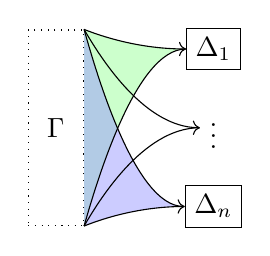
\begin{tikzpicture}[baseline]
    \path
    (-1,1) node (Gtop) {}
    (-1,0) node (G) {$\Gamma$}
    (-1,-1) node (Gbot) {}
    ;
    \node[draw,dotted,fit=(Gtop) (G) (Gbot)] (GG) {};

    \path
    (1,1) node[draw] (Dtop) {$\Delta_1$}
    (1,0) node (D) {$\vdots$}
    (1,-1) node[draw] (Dbot) {$\Delta_n$}
    ;

    \fill[green!20!white,opacity=1] (GG.north east)
    parabola[bend at end] (Dtop.west)
    parabola[bend at start] (GG.south east)
    -- cycle;
    \fill[blue!40!white,opacity=.5] (GG.north east)
    parabola[bend at end] (Dbot.west)
    parabola[bend at start] (GG.south east)
    -- cycle;

    \draw[->] (GG.north east) parabola[bend at end] (Dtop.west);
    \draw (GG.south east) parabola[bend at end] (Dtop.west);
    \draw[->] (GG.north east) parabola[bend at end] (D.west);
    \draw (GG.south east) parabola[bend at end] (D.west);
    \draw[->] (GG.north east) parabola[bend at end] (Dbot.west);
    \draw (GG.south east) parabola[bend at end] (Dbot.west);
  \end{tikzpicture}
\end{displaymath}

To see how this definition works, let us construct an example substitution:
$A, B \to C, B \Longrightarrow B, C$.
Because the codomain is a Cartesian product, it suffices to give two separate
substitutions, $A, B \to C, B \Longrightarrow B$ and
$A, B \to C, B \Longrightarrow C$, with a substitution into a singleton
context being just a term.
We indeed have terms $x : A, y : B \to C, z : B \vdash y : B$ and
$x : A, y : B \to C, z : B \vdash y\,z : C$.
It is also instructive to look at an identity substitution (which is also a
renaming), $A, B \Longrightarrow A, B$, witnessed by terms
$x : A, y : B \vdash x : A$ and $x : A, y : B \vdash y : B$.

When working with our semiring-annotated calculus \name{}, contexts are no
longer understood as Cartesian products.
This means that substitutions of type $\Gamma \Longrightarrow \Delta$ are no
longer equivalent to collections of substitutions
$\Gamma \Longrightarrow \Delta_i$.
Indeed, notice that we should still have an identity substitution of type
$\gr1A, \gr1B \Longrightarrow \gr1A, \gr1B$, but we do not have terms proving
either $\gr1A, \gr1B \vdash A$ or $\gr1A, \gr1B \vdash B$.
What we do have are terms $x : \gr1A, y : \gr0B \vdash x : A$ and
$x : \gr0A, y : \gr1B \vdash y : B$, and if we pointwise add together the
annotations of the two terms, we get back the original context
$x : \gr1A, y : \gr1B$.
Furthermore, adding up the annotations is not just a random operation;
linear contexts are understood to be tensor products of their elements, and
introduction rule for the tensor product involves summing the annotations of
the two sides.

For any annotated context $\Delta$, we have
$\Delta \vdash \bigotimes_{(\gr rx : A) \in \Delta}\oc\gr rA$ by iterated
application of $\otimes$-I with $\oc$-I and Var at the leaves.
Let $\Gamma = \grP\gamma$ and $\Delta = \grQ\delta$.
If we are to produce substitutions from $\Gamma$ to $\Delta$ in this
pattern, we simulate the applications of $\otimes$-I by producing, for each
element in $\Delta$, a usage context for $\gamma$ such that the whole collection
sums to $\grP$, then simulate the applications of $\oc$-I by dividing each of
the new usage contexts by the corresponding annotation in $\Delta$, calling
the divided usage contexts $\gr\Psi_x$, and finally, instead of a variable
from $\delta$, we give a term of type $\gr\Psi_x\gamma \vdash \delta_x$.
In summary, the constraint on the collection of usage contexts $\gr\Psi$ is
that $\grP = \sum_{(\gr rx : A) \in \Delta}\gr r\gr\Psi_x$.
Moreover, if we take $\grP$ and $\grQ$ to be row vectors and $\gr\Psi$ to be a
matrix, the latter expression is equal to the vector-matrix multiplication
$\grQ\gr\Psi$.
The resulting definition of simultaneous substitution is depicted below.

\begin{displaymath}
  \begin{tikzpicture}[baseline]
    \path
    (-1,1) node (Gtop) {}
    (-1,0) node (G) {$\grP\gamma$}
    (-1,-1) node (Gbot) {}
    ;
    \node[draw,dotted,fit=(Gtop) (G) (Gbot)] (GG) {};

    \path
    (1,1) node (Dtop) {}
    (1,0) node (D) {$\grQ\delta$}
    (1,-1) node (Dbot) {}
    ;
    \node[draw,dotted,fit=(Dtop) (D) (Dbot)] (DD) {};

    \draw[->,double] (GG) -- (DD);
  \end{tikzpicture}
  \coloneqq
  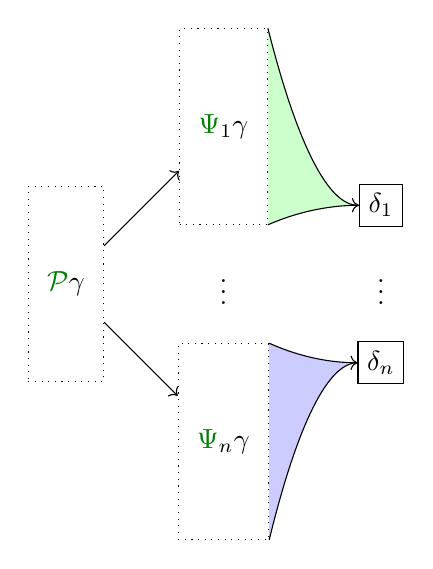
\begin{tikzpicture}[baseline]
    \path
    (-1,1) node (Gtop) {}
    (-1,0) node (G) {$\grP\gamma$}
    (-1,-1) node (Gbot) {}
    ;
    \node[draw,dotted,fit=(Gtop) (G) (Gbot)] (GG) {};

    \path
    (1,3) node (G1top) {}
    (1,2) node (G1) {$\gr\Psi_1\gamma$}
    (1,1) node (G1bot) {}
    ;
    \node[draw,dotted,fit=(G1top) (G1) (G1bot)] (GG1) {};
    \draw[->] (GG) -- (GG1);

    \path (1,0) node {$\vdots$};

    \path
    (1,-1) node (Gntop) {}
    (1,-2) node (Gn) {$\gr\Psi_n\gamma$}
    (1,-3) node (Gnbot) {}
    ;
    \node[draw,dotted,fit=(Gntop) (Gn) (Gnbot)] (GGn) {};
    \draw[->] (GG) -- (GGn);

    \path
    (3,1) node[draw] (Dtop) {$\delta_1$}
    (3,0) node (D) {$\vdots$}
    (3,-1) node[draw] (Dbot) {$\delta_n$}
    ;

    \fill[green!20!white] (GG1.north east)
    parabola[bend at end] (Dtop.west)
    parabola[bend at start] (GG1.south east)
    -- cycle;
    \draw[->] (GG1.north east) parabola[bend at end] (Dtop.west);
    \draw (GG1.south east) parabola[bend at end] (Dtop.west);

    \fill[blue!20!white] (GGn.north east)
    parabola[bend at end] (Dbot.west)
    parabola[bend at start] (GGn.south east)
    -- cycle;
    \draw[->] (GGn.north east) parabola[bend at end] (Dbot.west);
    \draw (GGn.south east) parabola[bend at end] (Dbot.west);
  \end{tikzpicture}
  \quad\textrm{where }\grP = \grQ\gr\Psi
\end{displaymath}

In type theory, we write out the definition as follows.

\begin{displaymath}
  \sum_{\gr\Psi : \size\Delta \to \size\Gamma \to \Ann}
    \left(\grP = \grQ\gr\Psi\right) \times
    \prod_{(x : A) \in \delta}\gr\Psi_x\gamma \vdash A
\end{displaymath}

We can see the step-by-step construction of a substitution play out by adapting
the previous example to have type
$\gr0A, \gr2(B \multimap C), \gr3B \Longrightarrow \gr1B, \gr2C$.
To split the goal up, we note that $
\begin{pmatrix} \gr0 & \gr2 & \gr3 \end{pmatrix} =
\begin{pmatrix} \gr0 & \gr0 & \gr1 \end{pmatrix} +
\begin{pmatrix} \gr0 & \gr2 & \gr2 \end{pmatrix}
$, so it suffices to give substitutions of types
$\gr0A, \gr0(B \multimap C), \gr1B \Longrightarrow \gr1B$ and
$\gr0A, \gr2(B \multimap C), \gr2B \Longrightarrow \gr2C$.
Furthermore, our term calculus only supports $\gr1$-annotated conclusions,
so we divide the second substitution type through by $\gr2$.
Finally, we give the terms largely as before:
$\gr0x : A, \gr0y : B \to C, \gr1z : B \vdash y : B$ and
$\gr0x : A, \gr1y : B \to C, \gr1z : B \vdash z\,y : C$.

While we naturally derive a matrix as a fragmentation of a usage vector, we can
get a slightly cleaner presentation by instead using an abstract linear map.
Let $\gr\Psi$ now be a linear map of type
$\Ann^{\size\Delta} \to \Ann^{\size\Gamma}$, with application written postfix.
The equation $\grP = \grQ\gr\Psi$ remains unchanged.
Where we previously wrote $\gr\Psi_x$, the most direct replacement would be
$\langle x \rvert\gr\Psi$, with $\langle x \rvert$ being the $x$th basis row
vector.
But then we notice that $\langle x \rvert$ is exactly the $\grQprime$ satisfying
$\grQprime\delta \sqni x : B$.
This gives us the following definition, which can be verified by equationally
substituting $\grPprime$ and expanding the definition of $\sqni$.

\begin{displaymath}
  \sum_{\gr\Psi : \Ann^{\size\Delta} \to \Ann^{\size\Gamma}}
    \left(\grP = \grQ\gr\Psi\right) \times
    \prod_{A,\grQprime,\grPprime} \left(
    \grPprime = \grQprime\gr\Psi \to \grQprime\delta \sqni A \to
    \grPprime\gamma \vdash A\right)
\end{displaymath}

We now have a new reading for the interpretation of a linear substitution:
a linear map $\gr\Psi$ relating the two usage vectors $\grP$ and $\grQ$, and
for any two similarly related usage vectors $\grPprime$ and $\grQprime$, we
have a type-preserving function from variables in $\grQprime\delta$ to terms in
$\grPprime\gamma$.
Even though we don't use $\gr\Psi$ as a matrix containing fragmented usage
vectors, we can still justify why it should be a \emph{linear} map.
We need $\gr\Phi$ to respect all fragmentation of the usage context in a typing
rule, and we know that all such fragmentation is done by linear operations
zero, addition, and scaling by a constant.
\todo{Expand. Substitutions need to preserve everything done to the context,
and linear things are all we do to the context.}

Taking a lead from \cref{sec:kits}, we deduce a definition of
\emph{environment} by replacing the $\vdash$ in the definition of simultaneous
substitution by an arbitrary type family $\mathcal V$.
Letting $\mathcal V$ be $\sqni$ gives us a notion of simultaneous renaming,
allowing for renamings with types such as
$\gr6A, \gr0B, \gr1C \stackrel\sqni\Longrightarrow \gr1C, \gr2A, \gr4A$.

It is worth noting that, when contexts are Cartesian products, passing from
``a map into $\Delta$'' to ``for each $A \in \Delta$, a map into $A$'' does not
lose any generality because the universal property of Cartesian products
states that every map into a Cartesian product can be given factor-wise.
Hence, $\Delta$ and the one-element context $\prod_{A \in \Delta}A$ are
isomorphic in the category of contexts and simultaneous substitution.
However, tensor products are not limits, so don't have the same universal
property.
Indeed, many annotated contexts are not isomorphic to the weighted product of
their elements.
For example, we do not have a substitution of type
$\gr1(A \otimes B) \Longrightarrow \gr1A, \gr1B$ because we would first need
to pattern-match on the tensor product \emph{before} trying to derive the
target context.
This loss of generality is however justified when we consider the action of a
substitution.
Substitutions should only be replacing variables by terms, whereas if
substitutions were allowed to pattern-match before introducing the target, then
the substitution would have to replace the original term by a term that first
pattern-matches and then continues like the original term.

\section{Properties of linear environments}\label{sec:lenv}
\begin{remark}
  Given an environment $\rho : \grP\gamma \env\V \grQ\delta$ and a $\grPprime$
  and a $\grQprime$ such that $\grPprime = \grQprime\plr{\rho.\gr\Psi}$,
  there is also an environment of type $\grPprime\gamma \env\V \grQprime\delta$
  with the same linear map and action on variables.
\end{remark}
\begin{proof}
  The only part of the definition of an environment dependent on $\grP$ or
  $\grQ$ is the constraint $\grP = \grQ\gr\Psi$, which we are able to replace
  for $\grPprime$ and $\grQprime$.
\end{proof}

When constructing an environment, we can do so by cases on the shape of the
target context.
We can create an environment into the empty context when all usage annotations
on the source context are $\gr0$.
We can create an environment into a concatenated context when we can additively
split up the annotations of the source context and produce environments into
both halves from the split sources.
We can create an environment into a singleton context when there is a context
$\gr r$ times smaller than the source context in which we can produce a value
of the appropriate type.

\begin{lemma}\label{thm:construct-env}
  We can define all of the following equivalences for any values of the free
  variables.
  \begin{itemize}
    \item $\forallb{I \dotlr \plr{{-} \env\V {\cdot}}}$
    \item $\forallb{\plr{{-} \env\V \Gamma} \sep \plr{{-} \env\V \Delta}
      \dotlr \plr{{-} \env\V \Gamma, \Delta}}$
    \item
      $\forallb{\gr r \cdot \plr{\V\,(-)\,A} \dotlr \plr{{-} \env\V \gr rA}}$
  \end{itemize}
\end{lemma}
\begin{proof}
  There are 6 cases to check.
  Throughout, we write $\Gamma$ as $\grP\gamma$ and $\Delta$ as $\grQ\delta$
  when convenient.
  \begin{description}
    \item[$I(\to)$]
      Let $\gr\Psi$ be the unique linear map out of the zero space.
      By definition, $\gr0 = \grQ\gr\Psi$.
      There are no variables to act upon.
    \item[$I(\gets)$]
      $\grQ\gr\Psi$ is an empty sum, so if $\grP = \grQ\gr\Psi$ then
      $\grP = \gr0$.
    \item[$\sep(\to)$]
      Let the given environments be $\rho : \grRl\theta \env\V \Gamma$ and
      $\sigma : \grRr\theta \env\V \Delta$, with $\grR = \grRl + \grRr$.
      Define $\gr\Psi \coloneqq [\rho.\gr\Psi, \sigma.\gr\Psi]$, using the
      coproduct structure of the concatenated vector space.
      We have $\grR = \grRl + \grRr =
      \grP\plr{\rho.\gr\Psi} + \grQ\plr{\sigma.\gr\Psi} =
      \plr{\grP, \grQ}\gr\Psi$.
      To act on variables, we are given
      $\grRprime = \plr{\grPprime, \grQprime}\gr\Psi$ and
      $\grPprime\gamma, \grQprime\delta \sqni A$.
      Without loss of generality, let us have $\grPprime\gamma \sqni A$ and
      $\grQprime = \gr0$.
      Thus, $\grRprime = \grPprime\plr{\rho.\gr\Psi}$, and we can act on the
      variable using $\rho$.
    \item[$\sep(\gets)$]
      Let the unnamed context be $\Theta$, also written $\grR\theta$.
      The linear map
      $\gr\Psi : \Ann^{\size\Gamma + \size\Delta} \to \Ann^{\size\Theta}$ splits
      into
      $\gr\Psi_{\gr l} : \Ann^{\size\Gamma} \to \Ann^{\size\Theta}
      \coloneqq \langle \id, 0 \rangle; \gr\Psi$ and
      $\gr\Psi_{\gr r} : \Ann^{\size\Delta} \to \Ann^{\size\Theta}
      \coloneqq \langle 0, \id \rangle; \gr\Psi$, using the product structure of
      the concatenated vector space.
      Let $\grRl \coloneqq \grP\gr\Psi_{\gr l}$ and
      $\grRr \coloneqq \grQ\gr\Psi_{\gr r}$, by definition satisfying the
      required equations.
      For the action on variables, let us consider the left environment.
      We are given $\grRprime = \grPprime\gr\Psi_{\gr l}$ and
      $\grPprime\gamma \sqni A$.
      From these, we get
      $\grRprime = \grPprime\gr\Psi_{\gr l} = \plr{\grPprime, \gr0}\gr\Psi$ and
      $\grPprime\gamma, \gr0\delta \sqni A$.
      We can therefore act using the original environment.
    \item[$\cdot(\to)$]
      Let $\grP$ and $\grPprime$ be such that $\grP = \gr r\grPprime$ and let
      $v : \V\,\grPprime\gamma\,A$.
      Let $\gr\Psi : \Ann \to \Ann^{\size\gamma}
      \coloneqq \gr r\gr' \mapsto \gr r\gr'\grPprime$.
      By definition and the previous assumption, we have $\grP = \gr r\gr\Psi$.
      When acting on a variable, we have $\grP\gr{''} = \gr r\gr'\gr\Psi$
      and $\gr r\gr'A \sqni A'$.
      The latter tells us that $A = A'$ and $\gr r\gr' = \gr1$.
      Thus, $\grP\gr{''} = \grPprime$.
      We therefore need a value of type $\V\,\grPprime\gamma\,A$, which we can
      take to be $v$.
    \item[$\cdot(\gets)$]
      Let us have an environment of type $\grP\gamma \env\V \gr rA$.
      We want to use its action on variables to yield a value.
      To do this, we let $\grPprime \coloneqq \gr1\gr\Psi$, and use this
      equation, together with the fact that we have a variable of type
      $\gr1A \sqni A$, to get a value of type $\V\,\grPprime\gamma\,A$.
      Furthermore, we derive $\grP = \gr r\gr\Psi = \gr r\grPprime$, as
      required.
  \end{description}
\end{proof}

We could, indeed, use these three clauses to define what an environment is.
However, I find them difficult to work with, as it is often easier to do
linear algebraic proofs separately from the rest of an environment.
For identity and composition, as we are about to see, the original definition
is easier to use because we can rely on the identity and composition of linear
maps.
Concretely, an inductive proof of identity would, for example, involve
constructing an environment of type
$\grP\gamma, \grQ\delta \env\V \grP\gamma, \grQ\delta$ by constructing
environments of types $\grP\gamma, \gr0\delta \env\V \grP\gamma$ and
$\gr0\gamma, \grQ\delta \env\V \grQ\delta$.
These are not identity environments, so we would have to strengthen the
induction hypothesis.

One of the primary test cases for environments is simultaneous substitution,
which will look like the following rule.
The admissibility of substitution will be by induction on the derivation of
$\Delta \vdash A$, so we will need to be able to adapt any environment we are
given to work with any possible context of new premises.
In the simply typed case, the only change to the context we encountered was the
binding of new variables.
Now, with usage annotations, we furthermore have linear decompositions of the
context, necessitating changes to the environment whenever usage annotations
change.
I will deal first with linear decompositions.

\begin{displaymath}
  \begin{prooftree}
    \hypo{\Gamma \env{\vdash} \Delta}
    \hypo{\Delta \vdash A}
    \infer2[sub]{\Gamma \vdash A}
  \end{prooftree}
\end{displaymath}

There are three kinds of linear decompositions we have to deal with: zero,
addition, and scaling; corresponding to bunched connectives $I^*$, $\sep$, and
$\gr r \cdot {}$, respectively.
In each case, we have a simple preservation lemma, transforming an environment
of type $\Gamma \env\V \Delta$ and a decomposition of $\Delta$ into a
decomposition of $\Gamma$ and environments for all of the decomposed fragments
of $\Gamma$ and $\Delta$.

\begin{lemma}[environments preserve zero]\label{thm:lr-env-zero}
  Given an environment of type $\grP\gamma \env\V \grQ\delta$ such that
  $\grQ \leq \gr 0$, we also have that $\grP \leq \gr 0$.
\end{lemma}
\begin{proof}
  $\grP \leq \grQ\gr\Psi \leq \gr0\gr\Psi = \gr0$, by environment
  compatibility and monotonicity and linearity of $\gr\Psi$.
\end{proof}

\begin{lemma}[environments preserve addition]\label{thm:lr-env-add}
  Given an environment of type $\grP\gamma \env\V \grQ\delta$ such that
  $\grQ \leq \grQl + \grQr$ for some $\grQl$ and $\grQr$, we also have $\grPl$
  and $\grPr$ such that $\grP \leq \grPl + \grPr$ and there are environments
  of types $\grPl\gamma \env\V \grQl\delta$ and
  $\grPr\gamma \env\V \grQr\delta$.
\end{lemma}
\begin{proof}
  Let $\grPl \coloneqq \grQl\gr\Psi$ and $\grPr \coloneqq \grQr\gr\Psi$.
  Then, $\grP \leq \grQ\gr\Psi \leq \plr{\grQl + \grQr}\gr\Psi =
  \grQl\gr\Psi + \grQr\gr\Psi = \grPl + \grPr$, satisfying the first condition.
  Because clearly $\grPl \leq \grQl\gr\Psi$ and $\grPr \leq \grQr\gr\Psi$,
  \cref{thm:env-resize} on the original environment gives us the required
  pair of new environments.
\end{proof}

\begin{lemma}[environments preserve scaling]\label{thm:lr-env-scale}
  Given an environment of type $\grP\gamma \env\V \grQ\delta$ such that
  $\grQ \leq \gr r\grQprime$ for some $\grQprime$, we also have a $\grPprime$
  such that $\grP \leq \gr r\grPprime$ and there is an environment of type
  $\grPprime\gamma \env\V \grQprime\delta$.
\end{lemma}
\begin{proof}
  Let $\grPprime \coloneqq \grQprime\gr\Psi$.
  Then, $\grP \leq \grQ\gr\Psi \leq \plr{\gr r\grQprime}\gr\Psi =
  \gr r\plr{\grQprime\gr\Psi} = \gr r\grPprime$, satisfying the first condition.
  Because clearly $\grPprime \leq \grQprime\gr\Psi$,
  \cref{thm:env-resize} on the original environment gives us the required
  new environment.
\end{proof}

Finally, I will also take the opportunity to give the bind lemma, allowing
environments to incorporate newly bound variables.
In the intuitionistic case, the bind lemma had two requirements on $\V$: $\V$
admits weakening and we can map variables into $\V$-values.
With usage annotations, the former is unreasonable, but it turns out that we
only need weakening by variables whose usage annotation is less than or equal
to $\gr0$.
The latter stays as-is, with the note that ``variable'' now means a
usage-checked variable.

\begin{lemma}[bind]\label{thm:lr-bind}
  Given functions
  ${\swarrow^k} : \forall \Gamma, \grR, \theta.~\grR \leq \gr0 \to
  \forallb{\V\,\Gamma \dotto \V\,\plr{\Gamma, \grR\theta}}$ and
  $\mathrm{vr} : \forallb{{\sqni} \dotto \V}$, we can turn an environment of
  type $\Gamma \env\V \Delta$ into an environment of type
  $\Gamma, \Theta \env\V \Delta, \Theta$ for any context $\Theta$.
\end{lemma}
\begin{proof}
  Let $\grP\gamma \coloneqq \Gamma$, $\grQ\delta \coloneqq \Delta$, and
  $\grR\theta \coloneqq \Theta$.
  Let the new linear map $\gr\Psi\gr' : \Ann^{\size\Delta + \size\Theta} \to
  \Ann^{\size\Gamma + \size\Theta}$ be $\gr\Psi \oplus \gr I$.
  That is, in block matrix notation,
  $\begin{pmatrix} \gr\Psi & \gr0 \\ \gr0 & \gr I \end{pmatrix}$.
  Checking that this linear map fits, we have
  $\begin{pmatrix}\grP & \grR\end{pmatrix}
  \leq \begin{pmatrix}\grQ\gr\Psi & \grR\gr I\end{pmatrix}
  = \begin{pmatrix}\grQ & \grR\end{pmatrix}\plr{\gr\Psi \oplus \gr I}$.
  For the action on variables, we are given vectors $\grPprime$,
  $\grR\gr'_\grP$, $\grQprime$, and $\grR\gr'_\grQ$ such that
  $\begin{pmatrix} \grPprime & \grR\gr'_\grP \end{pmatrix} \leq
  \begin{pmatrix} \grQprime & \grR\gr'_\grQ \end{pmatrix}
  \plr{\gr\Psi \oplus \gr I}$ and we have a variable of type
  $\grQprime\delta, \grR\gr'_\grQ\theta \sqni A$ for some type $A$.
  The constraint on the new vectors reduces to $\grPprime \leq \grQprime\gr\Psi$
  and $\grR\gr'_\grP \leq \grR\gr'_\grQ$.
  From the variable we either have a variable $x$ in $\delta$ with
  $\grQprime \leq \langle x \rvert$ and $\grR\gr'_\grQ \leq \gr0$, or a
  variable $y$ in $\theta$ with $\grQprime \leq \gr0$ and
  $\grR\gr'_\grQ \leq \langle y \rvert$.
  In the former case, the action of the original environment on $x$ gives us a
  $\V$-value in $\grPprime\gamma$, and the $\gr0$-weakening principle
  $\swarrow^k$, noting that $\grR\gr'_\grP \leq \grR\gr'_\grQ \leq \gr0$, gives
  us a $\V$-value in $\grPprime\gamma, \grR\gr'_\grP\theta$.
  In the latter case, we have that
  $\begin{pmatrix} \grPprime & \grR\gr'_\grP \end{pmatrix}
  \leq \begin{pmatrix} \grQprime\gr\Psi & \grR\gr'_\grQ \end{pmatrix}
  \leq \begin{pmatrix} \gr0\gr\Psi & \langle y \rvert \end{pmatrix}
  = \begin{pmatrix} \gr0 & \langle y \rvert \end{pmatrix}
  = \left\langle {\searrow}y \right\rvert$, so $y$ also serves as a
  usage-checked variable in $\grPprime\gamma, \grR\gr'_\grP\theta$.
  From this usage-checked variable, we get a $\V$-value in the same context
  using $\mathrm{vr}$.
\end{proof}

The requirements for identity and composition of environments look a bit like
the unit and lift of a Kleisli triple.

\begin{lemma}[Identity environment]
  Given a function $\mathrm{vr} : \forallb{{\sqni} \dotto \V}$, for any
  $\Gamma$ we have an environment of type $\Gamma \env\V \Gamma$.
\end{lemma}
\begin{proof}
  Let $\gr\Psi$ be the identity map, which clearly satisfies
  $\grP = \grP\gr\Psi$.
  When acting on a variable, the equation $\grPprime = \grQprime\gr\Psi$ means
  that $\grPprime = \grQprime$, so we want, from a variable of type
  $\grPprime\gamma \sqni A$, a value of type $\V\,\grPprime\gamma\,A$, which
  we can get from $\mathrm{vr}$.
\end{proof}

\begin{lemma}\label{thm:env-comp-lemma}
  Given an environment $\rho : \Gamma \env\U \Delta$ for which we have, for any
  $\grPprime$ and $\grQprime$ such that
  $\grPprime = \grQprime\plr{\rho.\gr\Psi}$, we have a function
  $\mathrm{lift}_\rho :
  \forallb{\V\,\grQprime\delta \dotto \W\,\grPprime\gamma}$,
  we can map environments of type $\Delta \env\V \Theta$ into environments of
  type $\Gamma \env\W \Theta$.
\end{lemma}
\begin{proof}
  Let $\rho$ be as in the statement, and let $\sigma : \Delta \env\V \Theta$.
  For the environment we are constructing, let
  $\gr\Psi \coloneqq \sigma.\gr\Psi; \rho.\gr\Psi$, noting that
  $\grP = \grQ\plr{\rho.\gr\Psi} =
  \plr{\grR\plr{\sigma.\gr\Psi}}\plr{\rho.\gr\Psi}$.
  For the action on variables, we are given $\grPprime = \grRprime\gr\Psi$ with
  $\grRprime\theta \sqni A$.
  We can immediately apply the action of $\sigma$, giving us a value of type
  $\V\,\plr{\grRprime\plr{\sigma.\gr\Psi}}\,A$.
  We note that
  $\grPprime = \plr{\grRprime\plr{\sigma.\gr\Psi}}\plr{\rho.\gr\Psi}$, and
  apply $\mathrm{lift}_\rho$ to get the desired value.
\end{proof}

\begin{corollary}[Composition of environments]
  Given a function
  $\mathrm{lift} : \plr{\rho : \grP\gamma \env\U \grQ\delta} \to
  \forall \grPprime, \grQprime.~\grPprime = \grQprime\plr{\rho.\gr\Psi} \to
  \forallb{\V\,\grQprime\delta \dotto \W\,\grPprime\gamma}$, then we can
  compose environments of types $\Gamma \env\U \Delta$ and
  $\Delta \env\V \Theta$ into an environment of type $\Gamma \env\W \Theta$.
\end{corollary}

\begin{example}
  We can derive the following instances of environment composition.
  \begin{itemize}
    \item If $\U = \V = \W = {\sqni}$, then $\mathrm{lift}$ is given by the
      action of the renaming $\rho$ on variables.
      This allows us to derive composition of renamings.
    \item More generally, if $\V = {\sqni}$ and $\U = \W$, we can still use
      the action of the environment $\rho$.
      This means that renamings post-compose with any other sort of environment.
    \item If $\V = \W = {\vdash}$, then $\mathrm{lift}$ is given by a
      syntactic traversal.
      For example, if $\U = {\sqni}$, we need the action of renaming on terms
      to show that a renaming followed by a substitution composes to a
      substitution.
      If $\U = {\vdash}$, then the action of substitution on terms gives us that
      substitutions compose.
    \item More generally, if $\V = {\vdash}$ and we have a semantics from
      $\U$ to $\W$, then $\mathrm{lift}$ can be given by the semantic traversal
      of terms.
  \end{itemize}
\end{example}

% Concatenation is difficult; save to after I've talked about renamings.

% Finally for this section, we give the conditions under which the
% context-forming operations (empty, concatenation, and singleton) have a
% functorial action with respect to $\V$-environments.
%
% \begin{lemma}
%   For any $\V$, there is an environment ${\cdot} \env\V {\cdot}$.
% \end{lemma}
% \begin{proof}
%   By \autoref{thm:construct-env}, it suffices to show $I\,{\cdot}$, which is
%   trivially true.
% \end{proof}

\section{Substitution is admissible in \name{}}\label{sec:lrsub}
\def\LRKits{../agda/processed-latex/LRKits.tex}

I can now show that, using the notion of \emph{environment} derived in
\cref{sec:lrkits}, we can replicate the Agda proofs from
\cref{sec:syntactic-kits} in the usage-aware setting of $\name$.
From \cref{sec:lenv}, we know that environments are preserved under all
syntax-forming operations: zero, addition, scaling, and binding.
What is left is to show how these properties are deployed, and also how to
go on and prove the admissibility of simultaneous renaming, simultaneous
substitution, and then single substitution.

There are a few notational changes necessary in the Agda code, compared to the
typeset mathematics above.
Usage vectors, elsewhere called $\grP$, $\grQ$, and $\grR$ are rendered as
\AgdaBound{P}, \AgdaBound{Q}, and \AgdaBound{R}, respectively.
Usage contexts and typing contexts are tied together with the
\AgdaInductiveConstructor{ctx} constructor, rather than simple juxtaposition.
Environments, elsewhere notated $\Gamma \env\V \Delta$, are rendered as
\AgdaRecord{[}\AgdaSpace{}\AgdaBound{$\V$}\AgdaSpace{}\AgdaRecord{]}%
\AgdaSpace{}\AgdaBound{$\Gamma$}\AgdaSpace{}\AgdaRecord{$\Rightarrow^e$}%
\AgdaSpace{}\AgdaBound{$\Delta$}.

We start with a slightly modified definition of \AgdaRecord{Kit}.
We saw in \cref{thm:lr-bind} that in the usage-annotated context, we restrict
weakening of $\V$-values to just $\gr0$-use variables.
Meanwhile, the function $\mathrm{vr}$, also seen in \cref{thm:lr-bind}, maps
usage-checked variables to $\V$-values, and the function $\mathrm{tm}$, used
to coerce $V$-values yielded by the environment into terms, stays the same.
I state weakening in a slightly different way than previously, so as to help
unification against a known result type (avoiding the problem described by
\citet{McBride12} as \emph{green slime}).
The type \AgdaFunction{Weakening}\AgdaSpace{}\AgdaBound{$\V$} can be read as
saying that, for any context $\grP\gamma$ of shape $s + t$, if the right of
$\grP$ is below $\gr0$, then a value in the left part of $\grP\gamma$ weakens
to a value in the whole of $\grP\gamma$.

\ExecuteMetaData[\LRKits]{Kit}

To demonstrate the important points succinctly, I cut \name{} down to just the
$\oc\gr r$-fragment.
The introduction rule and pattern-matching eliminator feature scaling, addition,
and variable binding, missing out only on sharing (which is trivial) and zero
(which is simpler than, and analogous to, addition).
The resulting type of well typed terms is below.

\ExecuteMetaData[\LRKits]{Tm}

Given a \AgdaRecord{Kit}, \cref{thm:lr-bind} looks like the following.
The \AgdaField{lookup} clauses still contain essentially the same structure as
in the intuitionistic case: discriminating on whether the variable is old or
new, using the given environment \AgdaBound{$\rho$} and weakening on the old
variables, and using \AgdaField{vr} to repackage new variables.
I will not explain any of the algebraic manipulations here; see
\cref{thm:lr-bind}.

\ExecuteMetaData[\LRKits]{bindEnv}

Given \AgdaFunction{bindEnv} (\cref{thm:lr-bind}), \AgdaFunction{env-+}
(\cref{thm:lr-env-add}), and \AgdaFunction{env-*} (\cref{thm:lr-env-scale}),
we can reproduce the syntactic traversal \AgdaFunction{trav}.
With all these lemmas in place, writing \AgdaFunction{trav}
becomes routine.
When processing a rule, we work our way up through the
premise connectives, applying \AgdaFunction{env-*} wherever we see a
\AgdaFunction{$\cdot^c$}, \AgdaFunction{env-+} wherever we see a
\AgdaFunction{$*^c$}, and \AgdaFunction{bindEnv} wherever we see a
\AgdaFunction{Bind}.
We then use whatever environments (with names beginning with
\AgdaBound{$\rho$}) and whatever usage vector splitting facts (with names
beginning with \AgdaBound{sp}) come out of this process to recursively
traverse the subterms and recombine the results.

\ExecuteMetaData[\LRKits]{trav}

Instantiating the generic syntactic traversal \AgdaFunction{trav} to renaming
looks just like it did in the intuitionistic case.
I have consistently replaced intuitionistic variables by linear variables, so
\AgdaFunction{id} and \AgdaInductiveConstructor{var} still work to embed
variables into variables and terms, respectively.
Weakening for variables \AgdaFunction{$\swarrow^v$} (not pictured) has been
updated to note that, for $\grP \leq \bra x$ and $\grR \leq \gr0$, we also have
$\begin{pmatrix} \grP & \grR \end{pmatrix} \leq \bra{{\swarrow}x}$.

\ExecuteMetaData[\LRKits]{var-kit}

In the intuitionistic case, environments were just functions, so we passed the
variable weakening function \AgdaFunction{$\swarrow^v$} to the function
\AgdaFunction{ren} to yield a term weakening function.
However, a usage-aware environment is a function packed together with usage
distribution data.
As such, we must make an environment version of \AgdaFunction{$\swarrow^v$}.
I start with a general lemma \AgdaFunction{$\swarrow$\^{}Env}, stating that if
$\V$ supports weakening, then so do $\V$-environments (in their domain
context).
This lemma then specialises to variables, with the identity renaming
\AgdaFunction{id\^{}Env} on the left part of the context and the proof
\AgdaBound{R0} that the right part of the context is below $\gr0$ combining
to give the desired weakening environment.

\ExecuteMetaData[\LRKits]{dlv-env}

This is what we need to instantiate \AgdaFunction{trav} for substitution.
As a reminder, I also give the type of \AgdaFunction{sub} in rule form.

\ExecuteMetaData[\LRKits]{sub}
\[
  \ebrule{%
    \hypo{\Gamma \env\vdash \Delta}
    \hypo{\Delta \vdash B}
    \infer2[sub]{\Gamma \vdash B}
  }
\]

Finally, the simultaneous substitution \AgdaFunction{sub} specialises to
single substitution \AgdaFunction{sub[-]}.
Single substitution is stated as an admissible rule below.
To substitute in for $\gr r$-many $A$ in the second term, we need to derive
one $A$ with usages $\grP$, and then assert that the result can handle the
usages of the original term $\grQ$, plus $\gr r$-many copies of $\grP$.

\[
  \ebrule{%
    \hypo{\grR \leq \grQ + \gr r\grP}
    \hypo{\grP\gamma \vdash A}
    \hypo{\grQ\gamma, \gr rA \vdash B}
    \infer3[singleSub]{\grR\gamma \vdash B}
  }
\]

The proof strategy for producing the substitution \AgdaFunction{$\sigma$} is
to proceed structurally on the codomain context $\grQ\gamma, \gr rA$ using
\cref{thm:construct-env}, applying the identity substitution
\AgdaFunction{id\^{}Env} on the $\gamma$ half, and dropping the term
\AgdaBound{t} in place of the variable we are substituting for.

\ExecuteMetaData[\LRKits]{subSingle}

\section{Recursion}\label{sec:rec}
Based on an intuitive understanding of ``usage'', recursion introduces a new
phenomenon relative to the forms of programs we have seen so far:
terms can be used an unbounded number of times.
For example, notice the following reduction in Agda.

\missingfigure{\texttt{foldr \_+\_ 0 (1 :: 2 :: 3 :: []) = 1 + (2 + (3 + 0))}}

The function \AgdaFunction{\_+\_} has been copied into 3 different places in
the running of the program.
This copying is despite no type telling us that \AgdaFunction{\_+\_} would be
used 3 times (both \verb|[1,2,3]| and \verb|[2,3]| have type
\AgdaDatatype{List}\AgdaSpace{}\AgdaDatatype{$\mathbb N$}, despite the
corresponding folds using \AgdaFunction{\_+\_} a different number of times).
As such, when checking an application of \AgdaFunction{foldr}, we need check
that we can use its functional argument (\AgdaFunction{\_+\_} in this case) an
arbitrary number of times.
If we were to fix $\Ann$ as the $\{\gr0, \gr1, \gr\omega\}$ posemiring, then
wrapping the type of the functional argument in $\oc\gr\omega$ would suffice.
However, we want to remain generic in the choice of semiring.

I propose the following additions to \name{} to support a broad class of
inductive types.
I define strictly positive functors syntactically, with the only notable
restriction being not being allowed to use the type variable $X$ in the domain
of a function type.
I then add least fixed points of such strictly positive functors to the syntax
of types.

\begin{align*}
  U &\Coloneqq A \multimap (-) \mid \oc\gr r(-) \\
  {\odot} &\Coloneqq {\otimes} \mid {\oplus} \mid {\with} \\
  F[X], G[X] &\Coloneqq X \mid A \mid U(F[X]) \mid F[X] \odot G[X] \\
  A &\Coloneqq \cdots \mid \mu X.~F[X]
\end{align*}

\begin{example}
  We may define $\mathrm{List}_A \coloneqq \mu X.~I \oplus \plr{A \otimes X}$.
\end{example}

In the typing rules, introduction of an inductive type is standard.
For the elimination rule, we follow a similar pattern to other pattern-matching
rules --- $\oplus$-E, $\otimes$-E, and $\oc$-E --- by splitting the context
and typing the eliminand in one half ($\grP$).
We type the continuation in the other half, but because the continuation may
be used multiple times, and in a modal context, we require that $\grQ$ is
preserved by all linear operations.

\begin{displaymath}
  \begin{prooftree}
    \hypo{\grR\gamma \vdash F[\mu X.~F[X]]}
    \infer1[$\mu$-I]{\grR\gamma \vdash \mu X.~F[X]}
  \end{prooftree}
\end{displaymath}
\begin{displaymath}
  \begin{prooftree}
    \hypo{\grR \leq \grP + \grQ}
    \hypo{\grP\gamma \vdash \mu X.~F[X]}
    \hypo{%
      \begin{matrix*}[l]
        \grQ \leq \gr0 \\
        \grQ \leq \grQ + \grQ \\
        \forall \gr r.~\grQ \leq \gr r\grQ
      \end{matrix*}%
    }
    \hypo{\grQ\gamma, \gr1F[C] \vdash C}
    \infer4[$\mu$-E]{\grR\gamma \vdash C}
  \end{prooftree}
\end{displaymath}

\begin{example}\label{thm:list-rules}
  For lists, we can derive the following introduction and elimination rules
  (with usage constraints omitted for brevity when obvious).

  \begin{align*}
    \begin{prooftree}
      \hypo{\grR \leq \gr0}
      \infer1[$I$-I]{I}
      \infer1[$\oplus$-I$_0$]%
      {\grR\gamma \vdash I \oplus \plr{A \otimes \mathrm{List}_A}}
      \infer1[$\mu$-I]{\grR\gamma \vdash \mathrm{List}_A}
    \end{prooftree}
    &&
    \begin{prooftree}
      \hypo{\grR \leq \grP + \grQ}
      \hypo{\grP\gamma \vdash A}
      \hypo{\grQ\gamma \vdash \mathrm{List}_A}
      \infer3[$\otimes$-I]{\grR\gamma \vdash A \otimes \mathrm{List}_A}
      \infer1[$\oplus$-I$_1$]%
      {\grR\gamma \vdash I \oplus \plr{A \otimes \mathrm{List}_A}}
      \infer1[$\mu$-I]{\grR\gamma \vdash \mathrm{List}_A}
    \end{prooftree}
  \end{align*}
  \begin{displaymath}
    \begin{prooftree}
      \hypo{\grP\gamma \vdash \mathrm{List}_A}
      \infer0[Var]{\gr0\gamma, \gr1\plr{I \oplus \plr{A \otimes C}}
        \vdash I \oplus \plr{A \otimes C}}
      \hypo{\nabla^n}
      \hypo{\nabla^c}
      \infer3[$\oplus$-E]{\grQ\gamma, \gr1\plr{I \oplus \plr{A \otimes C}}
        \vdash C}
      \infer2[$\mu$-E]{\grR\gamma \vdash C}
    \end{prooftree}
  \end{displaymath}
  \begin{align*}
    \textrm{where }\nabla^n &\coloneqq
    \begin{prooftree}
      \infer0[Var]{\gr0\gamma, \gr1I \vdash I}
      \hypo{\grQ\gamma \vdash C}
      \infer1[Wk]{\grQ\gamma, \gr0I \vdash C}
      \infer2[$I$-E]{\grQ\gamma, \gr1I \vdash C}
      \infer1[Wk]{\grQ\gamma, \gr0\plr{I \oplus \plr{A \otimes C}}, \gr1I
        \vdash C}
    \end{prooftree}
    \\\\
    \textrm{and }\nabla^c &\coloneqq
    \begin{prooftree}
      \infer0[Var]{\gr0\gamma, \gr1\plr{A \otimes C} \vdash A \otimes C}
      \hypo{\grQ\gamma, \gr1A, \gr1C \vdash C}
      \infer1[Wk]{\grQ\gamma, \gr0\plr{A \otimes C}, \gr1A, \gr1C \vdash C}
      \infer2[$\otimes$-E]{\grQ\gamma, \gr1\plr{A \otimes C} \vdash C}
      \infer1[Wk]%
      {\grQ\gamma, \gr0\plr{I \oplus \plr{A \otimes C}}, \gr1\plr{A \otimes C}
        \vdash C}
    \end{prooftree}
  \end{align*}
\end{example}

Following \cref{sec:lnd}, I want to turn the ad hoc constraints on $\grP$,
$\grQ$, and $\grR$ into the result of some premise combinators.
To do this, I introduce a new combinator $\Box^{0{+}{\times}}$ defined below,
along with the resulting implicit-context typing rules.

\begin{align*}
  \plr{\Box^{0{+}{\times}}\,T}\grR \coloneqq
  \plr{\grR \leq \gr0} \times \plr{\grR \leq \grR + \grR} \times
  \plr{\forall \gr r.~\grR \leq \gr r\grR} \times T\,\grR
\end{align*}

\begin{align*}
  \begin{prooftree}[comb]
    \hypo{\vdash F[\mu X.~F[X]]}
    \infer1[$\mu$-I]{\vdash \mu X.~F[X]}
  \end{prooftree}
  &&
  \begin{prooftree}[comb]
    \hypo{\vdash \mu X.~F[X]}
    \hypo{\sep}
    \hypo{\Box^{0{+}{\times}}\plr{\gr1F[C] \vdash C}}
    \infer3[$\mu$-E]{\vdash C}
  \end{prooftree}
\end{align*}

\begin{example}
  We can state the rules for lists derived in \cref{thm:list-rules} as follows.
  \begin{align*}
    \begin{prooftree}[comb]
      \hypo{I^*}
      \infer1{\vdash \mathrm{List}_A}
    \end{prooftree}
    &&
    \begin{prooftree}[comb]
      \hypo{\vdash A}
      \hypo{\sep}
      \hypo{\vdash \mathrm{List}_A}
      \infer3{\vdash \mathrm{List}_A}
    \end{prooftree}
    &&
    \begin{prooftree}[comb]
      \hypo{\vdash \mathrm{List}_A}
      \hypo{\sep}
      \hypo{\Box^{0{+}{\times}}
        \plr{\vdash C\hskip0.75em\dottimes\hskip0.75em\gr1A, \gr1C \vdash C}}
      \infer3{\vdash C}
    \end{prooftree}
  \end{align*}
\end{example}

\section{Addendum: (lack of) partiality}\label{sec:part}
As we have seen, the way additive and multiplicative rules are
realised algebraically is related to models of separation logic.
Models of separation logic typically use \emph{partial} commutative monoids to
model a heap, so it is tempting to generalise the commutative monoid of
addition in our semirings to a \emph{partial} commutative monoid.
However, we find that the most natural notion of \emph{partial semiring} is
degenerate, in the sense that all partial semirings are actually (total)
semirings.

Recall that a commutative monoid (or commutative monoid object) can be
defined in any symmetric monoidal category.
A partial commutative monoid is exactly a commutative monoid object in the
category of sets and partial functions with the usual monoidal product given
by pairing of objects and morphisms (like the Cartesian product in $\Set$).
However, semirings need a Cartesian category in order to state the interaction
equations between addition and multiplication.
While the category of sets and partial functions is not Cartesian, the
standard way to manufacture a Cartesian category out of a symmetric monoidal
category $\mathcal C$ is to take the category of cocommutative comonoids
$\mathrm{CComon}(\mathcal C)$.
Intuitively, the cocommutative comonoid structure equips the underlying
object $M$ with a \emph{delete} map $\eta : M \to I$ and a \emph{duplicate}
map $\delta : M \to M \otimes M$ which are coherent with respect to each other.
All morphisms in $\mathrm{CComon}(\mathcal C)$ must respect $\eta$ and
$\delta$; in particular, both addition and multiplication must separately
form bimonoids in $\mathcal C$ together with the cocommutative comonoid.

The distributivity laws of semirings are stated below.
I include these to show that the cocommutative comonoids of a monoidal category
give enough structure to state these laws.
The other laws --- that all morphisms respect $\eta$ and $\delta$, that addition
forms a commutative monoid, and that multiplication forms a monoid --- are
standard in symmetric monoidal category theory.

\[
  \begin{tikzpicture}[baseline]
    \path
    (-1,1) node(0) {0}
    (1,2) node(x) {}
    (0,0) node(*) {*}
    (0,-1) node(res) {}
    ;

    \draw (0) -- (*);
    \draw (x) to[out=270,in=45] (*);
    \draw (*) -- (res);
  \end{tikzpicture}
  =\quad
  \begin{tikzpicture}[baseline]
    \path
    (0,0) node(0) {0}
    (0,2) node(x) {}
    (0,-1) node(res) {}
    (0,1) node(del) {$\eta$}
    ;

    \draw (0) -- (res);
    \draw (x) -- (del);
  \end{tikzpicture}
  \quad=
  \begin{tikzpicture}[baseline]
    \path
    (1,1) node(0) {0}
    (-1,2) node(x) {}
    (0,0) node(*) {*}
    (0,-1) node(res) {}
    ;

    \draw (0) -- (*);
    \draw (x) to[out=270,in=135] (*);
    \draw (*) -- (res);
  \end{tikzpicture}
\]
\begin{displaymath}
  \begin{matrix}
    \begin{tikzpicture}[baseline]
      \path
      (-1,2) node(x) {}
      (0,2) node(y) {}
      (-0.5,1) node(+) {+}
      (1,2) node(z) {}
      (0,0) node(*) {*}
      (0,-1) node(res) {}
      ;

      \draw (x) to[out=270,in=135] (+);
      \draw (y) to[out=270,in=45] (+);
      \draw (+) to[out=270,in=135] (*);
      \draw (z) to[out=270,in=45] (*);
      \draw (*) -- (res);
    \end{tikzpicture}
    =
    \begin{tikzpicture}[baseline]
      \path
      (-2,3) node(x) {}
      (-1,3) node(y) {}
      (0,3) node(z) {}
      (0,2) node(dup) {$\delta$}
      (-1,1) node(x*) {*}
      (0,1) node(y*) {*}
      (-0.5,0) node(+) {+}
      (-0.5,-1) node(res) {}
      ;

      \draw (z) -- (dup);
      \draw (x) to[out=270,in=135] (x*);
      \draw (y) to[out=270,in=135] (y*);
      \draw (dup) to[out=-150,in=45] (x*);
      \draw (dup) -- (y*);
      \draw (x*) to[out=270,in=135] (+);
      \draw (y*) to[out=270,in=45] (+);
      \draw (+) -- (res);
    \end{tikzpicture}
    &\phantom{mmmm}&
    \begin{tikzpicture}[baseline]
      \path
      (1,2) node(x) {}
      (0,2) node(y) {}
      (0.5,1) node(+) {+}
      (-1,2) node(z) {}
      (0,0) node(*) {*}
      (0,-1) node(res) {}
      ;

      \draw (x) to[out=270,in=45] (+);
      \draw (y) to[out=270,in=135] (+);
      \draw (+) to[out=270,in=45] (*);
      \draw (z) to[out=270,in=135] (*);
      \draw (*) -- (res);
    \end{tikzpicture}
    =
    \begin{tikzpicture}[baseline]
      \path
      (2,3) node(x) {}
      (1,3) node(y) {}
      (0,3) node(z) {}
      (0,2) node(dup) {$\delta$}
      (1,1) node(x*) {*}
      (0,1) node(y*) {*}
      (0.5,0) node(+) {+}
      (0.5,-1) node(res) {}
      ;

      \draw (z) -- (dup);
      \draw (x) to[out=270,in=45] (x*);
      \draw (y) to[out=270,in=45] (y*);
      \draw (dup) to[out=-30,in=135] (x*);
      \draw (dup) -- (y*);
      \draw (x*) to[out=270,in=45] (+);
      \draw (y*) to[out=270,in=135] (+);
      \draw (+) -- (res);
    \end{tikzpicture}
  \end{matrix}
\end{displaymath}

It is well known that all commutative comonoids in $(\Set, \times)$, and indeed
any Cartesian monoidal category, are trivial, in the sense that every object of
$\Set$ gives rise to exactly one commutative comonoid.
We find in the following two lemmas that this property also holds of
$\plr{\Set_{\mathrm{part}}, \otimes}$.

\begin{lemma}\label{thm:ccomon-exists}
  For each object $X$ in $\plr{\Set_{\mathrm{part}}, {\otimes}}$, there is
  a cocommutative comonoid over $X$.
\end{lemma}
\begin{proof}
  Let $\eta(x) \coloneq ()$ and $\delta(x) \coloneq (x, x)$, with both
  being defined for all $x$.
  Checking that these satisfy the cocommutative comonoid laws is routine.
  Alternatively, we can see that both $\eta$ and $\delta$, being total, are
  morphisms in $\mathrm{Set}$, where it is well known that they form a
  cocommutative comonoid.
  The equations in $\mathrm{Set}$ carry over to $\mathrm{Set}_{\mathrm{part}}$.
\end{proof}

\begin{lemma}\label{thm:ccomon-unique}
  For each object $X$ in $\plr{\Set_{\mathrm{part}}, {\otimes}}$, any
  comonoid over $X$ is the one described in \cref{thm:ccomon-exists}.
\end{lemma}
\begin{proof}
  The left unit law says that, for all $x$ and $x'$, we have
  $\exists y.~\delta(x) = (y, x') \land \eta(y) = ()$ if and only if $x = x'$.
  Letting $x'$ be $x$ and reading from right to left, we get that there is
  some $y$ such that $\delta(x) = (y, x)$ and $\eta(y) = ()$.
  Symmetrically, from the right unit law, we get some $z$ such that
  $\delta(x) = (x, z)$ and $\eta(z) = ()$.
  But because $\delta$, being a partial function, is deterministic, we have
  $(y, x) = (x, z)$, giving us that $y = z = x$, and $\delta(x) = (x, x)$.
  Moreover, because the chosen $y$ is equal to $x$, we have for all $x$ that
  $\eta(x) = ()$.
\end{proof}

That a morphism $f$ respects the $\eta$ given in \cref{thm:ccomon-exists} is
equivalent to saying that $f$ is total.
Therefore, all possible semiring operators in
$\mathrm{CComon}\plr{\Set_{\mathrm{part}}, \otimes}$ are total, meaning that
there is a corresponding semiring in $\plr{\Set, \times}$.

The above reasoning shows that semirings in the category of sets and partial
functions are not worth studying.
If we want partiality, there appear to be two options.
The first option is to give up on multiplication.
We could imagine replacing the binary multiplication operator by a set of
unary modalities satisfying fewer laws.
In particular, I make little use of addition on the left of a multiplication,
and multiplying by $\gr0$ on the left (as done by $\oc\gr0$) is unwanted in some
cases (such as when encoding DILL and PD, as in \cref{sec:translation}).
With unary modalities, we could expect all of the required laws to be
expressible in a symmetric monoidal category.
The second option is to use a different notion of partiality.
The notion of partiality given by the category of sets and partial functions is
``strict'', in that composing with an everywhere-undefined function yields an
everywhere-undefined function.
With a non-strict notion of partial function, we may be able to have interesting
partial semirings.


\chapter{Renaming and substitution for $\name$}\label{sec:ren-sub-lr}

In \cref{sec:semirings}, I defined my calculus of interest $\name$.
In this chapter, I develop the necessary syntactic metatheory for
specifying and implementing the simultaneous substitution operation.
My aim in this chapter is to replay the development in \cref{sec:kits}, making
minimal changes to lemmas and theorems so as to support semiring usage
annotations.
The big change I make in this chapter is to the definition of
\emph{environment}.
In terms of ideas, I believe that the definition of environment I give in
\cref{sec:lrkits} is the main contribution of this thesis.
Its primary novel feature is the use of a linear map --- in the sense found in
linear algebra --- to distribute usage annotations across the values in the
environment.

The resulting substitution operation bears some similarity to a multi-variable
substitution operation given by \citet{petricek-thesis}.
This is the only other presentation I have found in the literature of an
operation similar to simultaneous substitution for a linear or linear-like
calculus.
I discuss Petricek's substitution lemma in more detail in \cref{sec:petricek}.
In brief, relative to Petricek's work, I extract the environment from the
substitution lemma, tidy up the definition, and present usage-annotated
environments as a reusable tool and object of study in their own right.
I reuse the resulting definition of environment in the remainder of this thesis,
taking advantage of the properties and generality of definition established in
this chapter, particularly in \cref{sec:semantics,sec:example-semantics}.

The body of this chapter starts with a motivation for and a definition of
environment in the usage-annotated setting in \cref{sec:lrkits}.
I then give some key properties of and operations on these environments in
\cref{sec:lenv}.
I apply the previous definitions and properties to the problems of simultaneous
renaming and substitution for $\name$ in \cref{sec:lrsub}, which also connects
the previous sections' mathematical developments with Agda code.
I then compare the yielded substitution operation with the one given by Petricek
in \cref{sec:petricek}, before a concluding discussion in
\cref{sec:ren-sub-lr-conc}.

\section{What are linear renaming and substitution?}\label{sec:lrkits}
\paragraph{New explanation}
Recalling from \cref{sec:kits}, we have the following definition of
\emph{environments} for simple types.

\begin{definition}[Simple environment]
  A $\V$-\emph{environment} between simply typed contexts $\Gamma$ and $\Delta$
  is a function, polymorphic in type $A$, from variables of type $A$ in
  $\Delta$ to inhabitants of $\V\,\Gamma\,A$.
  We write the type of such environments as $\Gamma \env\V \Delta$.
\end{definition}

\begin{definition}[Simple recursive environment]
  A \emph{recursive $\V$-environment} between simply typed contexts $\Gamma$ and
  $\Delta$ is defined by cases on the shape of $\Delta$ (where
  $\Gamma \env\V_R \Delta$ is the notation for the type of recursive
  environments for given $\V$, $\Gamma$, and $\Delta$):
  \begin{itemize}
    \item If $\Delta$ is empty, then there is one environment.
    \item If $\Delta$ is a concatenation $\Delta_l, \Delta_r$, then an
      environment is a pair of environments of types
      $\Gamma \env\V_R \Delta_l$ and $\Gamma \env\V_R \Delta_r$.
    \item If $\Delta$ is a singleton $A$, then an environment is a value of
      type $\V\,\Gamma\,A$.
  \end{itemize}
\end{definition}

\begin{definition}[Usage-annotated recursive environment]
  A \emph{recursive $\V$-environment} between annotated contexts $\Gamma$ and
  $\Delta$ is defined by cases on the shape of $\Delta$ (where
  $\Gamma = \grP\gamma$ and $\Gamma \env\V_R \Delta$ is the notation for the
  type of recursive environments for given $\V$, $\Gamma$, and $\Delta$):
  \begin{itemize}
    \item If $\Delta$ is empty, then an environment exists if $\grP = \gr0$.
    \item If $\Delta$ is a concatenation $\Delta_l, \Delta_r$, then an
      environment is a choice of usage vectors $\grPl$ and $\grPr$ such that
      $\grP = \grPl + \grPr$ and we have a pair of environments of types
      $\grPl\gamma \env\V_R \Delta_l$ and $\grPr\gamma \env\V_R \Delta_r$.
    \item If $\Delta$ is a singleton $\gr rA$, then an environment is a choice
      of a usage vector $\grPprime$ such that $\grP = \gr r\grPprime$ and we
      have a value of type $\V\,\grPprime\gamma\,A$.
  \end{itemize}
\end{definition}

From this definition, we can recover a functional-style definition by
separating choices of usage vectors from the provision of $\V$-values.
In particular, the only choices of usage vectors that are essential are the
$\grPprime$s in the singleton case, with the choices in the concatenation case
being determined as scalings and sums of these $\grPprime$s.
I let $\gr\Psi$ collect up these $\size\Delta$-many choices of
$\size\Gamma$-length usage vectors and note that the constraint on $\gr\Psi$
generated by all the scaling and summing is
$\grP = \sum_{\plr{x : \gr rA} \in \Delta} \gr r\gr\Psi_x$.

\begin{definition}[Usage-annotated environment (tentative)]
  A \emph{$\V$-environment} between annotated contexts $\Gamma$ and $\Delta$
  (written $\grP\gamma$ and $\grQ\delta$, respectively, when convenient)
  is a matrix $\gr\Psi : \Ann^{\size\Delta \times \size\Gamma}$ such that
  $\grP = \sum_{\plr{x : \gr rA} \in \Delta} \gr r\gr\Psi_x$ and for each
  $\plr{x : A} \in \delta$ we have a value of type $\V\,\gr\Psi_x\gamma\,A$.
\end{definition}

We may note, further, that the constraint
$\grP = \sum_{\plr{x : \gr rA} \in \Delta} \gr r\gr\Psi_x$ can be stated as the
vector-matrix multiplication $\grP = \grQ\gr\Psi$.
Using the same operation, we have that $\gr\Psi_x = \langle x \rvert\gr\Psi$.
Because $\langle x \rvert$ is exactly the $\grQprime$ such that
$\plr{x : A} \sqin \grQprime\delta$, we can rephrase the function producing
$\V$-values as: for each $A$, $\grPprime$, and $\grQprime$ such that
$\grPprime = \grQprime\gr\Psi$, a function from $\grQprime\delta \sqni A$ to
$\V\,\grPprime\gamma\,A$.
Finally, I choose to switch from matrices and matrix multiplication to
linear maps and their actions, which are easier to work with.
All of these changes yield my primary definition of an environment for
usage-annotated calculi.

\begin{definition}[Usage-annotated environment]
  A \emph{$\V$-environment} between annotated contexts $\Gamma$ and $\Delta$
  (written $\grP\gamma$ and $\grQ\delta$, respectively, when convenient)
  is a linear map $\gr\Psi : \Ann^{\size\Delta} \to \Ann^{\size\Gamma}$ (written
  postfix) such that $\grP = \grQ\gr\Psi$ and for each $A$, $\grPprime$, and
  $\grQprime$ such that $\grPprime = \grQprime\gr\Psi$, a function from
  $\grQprime\delta \sqni A$ to $\V\,\grPprime\gamma\,A$.
\end{definition}

\paragraph{Old explanation}
As we discussed in \cref{sec:kits}, simultaneous substitution gives a
notion of derivability of one context from another, while simultaneous renaming
gives a similar notion of derivability restricted to structural rules.
To adapt these notions from an intuitionistic setting to our substructural
setting, we must examine what it means to derive one context from another
substructually.

In the intuitionistic case, we say that to derive a context $\Delta$ from a
context $\Gamma$ is to derive each element $\Delta_i$ from $\Gamma$.
We may justify this by an intermediate step --- noting that contexts are
understood to be Cartesian products of their elements, and giving a map into
a Cartesian product is the same as giving a map into each factor.
I picture this definition as the diagram below.

\begin{displaymath}
  \begin{tikzpicture}[baseline]
    \path
    (-1,1) node (Gtop) {}
    (-1,0) node (G) {$\Gamma$}
    (-1,-1) node (Gbot) {}
    ;
    \node[draw,dotted,fit=(Gtop) (G) (Gbot)] (GG) {};

    \path
    (1,1) node (Dtop) {}
    (1,0) node (D) {$\Delta$}
    (1,-1) node (Dbot) {}
    ;
    \node[draw,dotted,fit=(Dtop) (D) (Dbot)] (DD) {};

    \draw[->,double] (GG) -- (DD);
  \end{tikzpicture}
  \coloneqq
  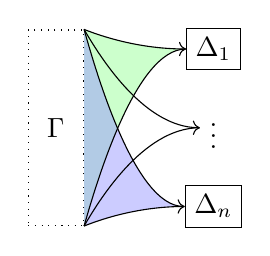
\begin{tikzpicture}[baseline]
    \path
    (-1,1) node (Gtop) {}
    (-1,0) node (G) {$\Gamma$}
    (-1,-1) node (Gbot) {}
    ;
    \node[draw,dotted,fit=(Gtop) (G) (Gbot)] (GG) {};

    \path
    (1,1) node[draw] (Dtop) {$\Delta_1$}
    (1,0) node (D) {$\vdots$}
    (1,-1) node[draw] (Dbot) {$\Delta_n$}
    ;

    \fill[green!20!white,opacity=1] (GG.north east)
    parabola[bend at end] (Dtop.west)
    parabola[bend at start] (GG.south east)
    -- cycle;
    \fill[blue!40!white,opacity=.5] (GG.north east)
    parabola[bend at end] (Dbot.west)
    parabola[bend at start] (GG.south east)
    -- cycle;

    \draw[->] (GG.north east) parabola[bend at end] (Dtop.west);
    \draw (GG.south east) parabola[bend at end] (Dtop.west);
    \draw[->] (GG.north east) parabola[bend at end] (D.west);
    \draw (GG.south east) parabola[bend at end] (D.west);
    \draw[->] (GG.north east) parabola[bend at end] (Dbot.west);
    \draw (GG.south east) parabola[bend at end] (Dbot.west);
  \end{tikzpicture}
\end{displaymath}

To see how this definition works, let us construct an example substitution:
$A, B \to C, B \Longrightarrow B, C$.
Because the codomain is a Cartesian product, it suffices to give two separate
substitutions, $A, B \to C, B \Longrightarrow B$ and
$A, B \to C, B \Longrightarrow C$, with a substitution into a singleton
context being just a term.
We indeed have terms $x : A, y : B \to C, z : B \vdash y : B$ and
$x : A, y : B \to C, z : B \vdash y\,z : C$.
It is also instructive to look at an identity substitution (which is also a
renaming), $A, B \Longrightarrow A, B$, witnessed by terms
$x : A, y : B \vdash x : A$ and $x : A, y : B \vdash y : B$.

When working with our semiring-annotated calculus \name{}, contexts are no
longer understood as Cartesian products.
This means that substitutions of type $\Gamma \Longrightarrow \Delta$ are no
longer equivalent to collections of substitutions
$\Gamma \Longrightarrow \Delta_i$.
Indeed, notice that we should still have an identity substitution of type
$\gr1A, \gr1B \Longrightarrow \gr1A, \gr1B$, but we do not have terms proving
either $\gr1A, \gr1B \vdash A$ or $\gr1A, \gr1B \vdash B$.
What we do have are terms $x : \gr1A, y : \gr0B \vdash x : A$ and
$x : \gr0A, y : \gr1B \vdash y : B$, and if we pointwise add together the
annotations of the two terms, we get back the original context
$x : \gr1A, y : \gr1B$.
Furthermore, adding up the annotations is not just a random operation;
linear contexts are understood to be tensor products of their elements, and
introduction rule for the tensor product involves summing the annotations of
the two sides.

For any annotated context $\Delta$, we have
$\Delta \vdash \bigotimes_{(\gr rx : A) \in \Delta}\oc\gr rA$ by iterated
application of $\otimes$-I with $\oc$-I and Var at the leaves.
Let $\Gamma = \grP\gamma$ and $\Delta = \grQ\delta$.
If we are to produce substitutions from $\Gamma$ to $\Delta$ in this
pattern, we simulate the applications of $\otimes$-I by producing, for each
element in $\Delta$, a usage context for $\gamma$ such that the whole collection
sums to $\grP$, then simulate the applications of $\oc$-I by dividing each of
the new usage contexts by the corresponding annotation in $\Delta$, calling
the divided usage contexts $\gr\Psi_x$, and finally, instead of a variable
from $\delta$, we give a term of type $\gr\Psi_x\gamma \vdash \delta_x$.
In summary, the constraint on the collection of usage contexts $\gr\Psi$ is
that $\grP = \sum_{(\gr rx : A) \in \Delta}\gr r\gr\Psi_x$.
Moreover, if we take $\grP$ and $\grQ$ to be row vectors and $\gr\Psi$ to be a
matrix, the latter expression is equal to the vector-matrix multiplication
$\grQ\gr\Psi$.
The resulting definition of simultaneous substitution is depicted below.

\begin{displaymath}
  \begin{tikzpicture}[baseline]
    \path
    (-1,1) node (Gtop) {}
    (-1,0) node (G) {$\grP\gamma$}
    (-1,-1) node (Gbot) {}
    ;
    \node[draw,dotted,fit=(Gtop) (G) (Gbot)] (GG) {};

    \path
    (1,1) node (Dtop) {}
    (1,0) node (D) {$\grQ\delta$}
    (1,-1) node (Dbot) {}
    ;
    \node[draw,dotted,fit=(Dtop) (D) (Dbot)] (DD) {};

    \draw[->,double] (GG) -- (DD);
  \end{tikzpicture}
  \coloneqq
  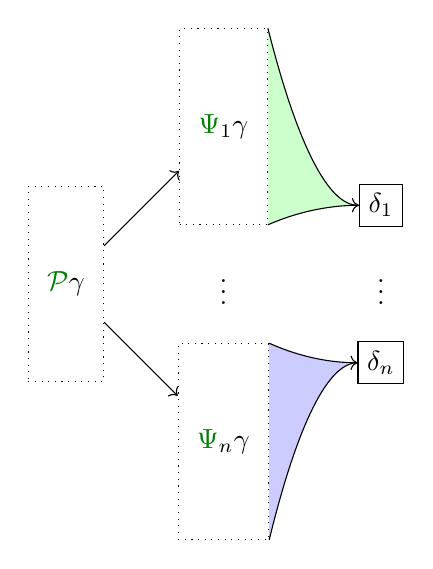
\begin{tikzpicture}[baseline]
    \path
    (-1,1) node (Gtop) {}
    (-1,0) node (G) {$\grP\gamma$}
    (-1,-1) node (Gbot) {}
    ;
    \node[draw,dotted,fit=(Gtop) (G) (Gbot)] (GG) {};

    \path
    (1,3) node (G1top) {}
    (1,2) node (G1) {$\gr\Psi_1\gamma$}
    (1,1) node (G1bot) {}
    ;
    \node[draw,dotted,fit=(G1top) (G1) (G1bot)] (GG1) {};
    \draw[->] (GG) -- (GG1);

    \path (1,0) node {$\vdots$};

    \path
    (1,-1) node (Gntop) {}
    (1,-2) node (Gn) {$\gr\Psi_n\gamma$}
    (1,-3) node (Gnbot) {}
    ;
    \node[draw,dotted,fit=(Gntop) (Gn) (Gnbot)] (GGn) {};
    \draw[->] (GG) -- (GGn);

    \path
    (3,1) node[draw] (Dtop) {$\delta_1$}
    (3,0) node (D) {$\vdots$}
    (3,-1) node[draw] (Dbot) {$\delta_n$}
    ;

    \fill[green!20!white] (GG1.north east)
    parabola[bend at end] (Dtop.west)
    parabola[bend at start] (GG1.south east)
    -- cycle;
    \draw[->] (GG1.north east) parabola[bend at end] (Dtop.west);
    \draw (GG1.south east) parabola[bend at end] (Dtop.west);

    \fill[blue!20!white] (GGn.north east)
    parabola[bend at end] (Dbot.west)
    parabola[bend at start] (GGn.south east)
    -- cycle;
    \draw[->] (GGn.north east) parabola[bend at end] (Dbot.west);
    \draw (GGn.south east) parabola[bend at end] (Dbot.west);
  \end{tikzpicture}
  \quad\textrm{where }\grP = \grQ\gr\Psi
\end{displaymath}

In type theory, we write out the definition as follows.

\begin{displaymath}
  \sum_{\gr\Psi : \size\Delta \to \size\Gamma \to \Ann}
    \left(\grP = \grQ\gr\Psi\right) \times
    \prod_{(x : A) \in \delta}\gr\Psi_x\gamma \vdash A
\end{displaymath}

We can see the step-by-step construction of a substitution play out by adapting
the previous example to have type
$\gr0A, \gr2(B \multimap C), \gr3B \Longrightarrow \gr1B, \gr2C$.
To split the goal up, we note that $
\begin{pmatrix} \gr0 & \gr2 & \gr3 \end{pmatrix} =
\begin{pmatrix} \gr0 & \gr0 & \gr1 \end{pmatrix} +
\begin{pmatrix} \gr0 & \gr2 & \gr2 \end{pmatrix}
$, so it suffices to give substitutions of types
$\gr0A, \gr0(B \multimap C), \gr1B \Longrightarrow \gr1B$ and
$\gr0A, \gr2(B \multimap C), \gr2B \Longrightarrow \gr2C$.
Furthermore, our term calculus only supports $\gr1$-annotated conclusions,
so we divide the second substitution type through by $\gr2$.
Finally, we give the terms largely as before:
$\gr0x : A, \gr0y : B \to C, \gr1z : B \vdash y : B$ and
$\gr0x : A, \gr1y : B \to C, \gr1z : B \vdash z\,y : C$.

While we naturally derive a matrix as a fragmentation of a usage vector, we can
get a slightly cleaner presentation by instead using an abstract linear map.
Let $\gr\Psi$ now be a linear map of type
$\Ann^{\size\Delta} \to \Ann^{\size\Gamma}$, with application written postfix.
The equation $\grP = \grQ\gr\Psi$ remains unchanged.
Where we previously wrote $\gr\Psi_x$, the most direct replacement would be
$\langle x \rvert\gr\Psi$, with $\langle x \rvert$ being the $x$th basis row
vector.
But then we notice that $\langle x \rvert$ is exactly the $\grQprime$ satisfying
$\grQprime\delta \sqni x : B$.
This gives us the following definition, which can be verified by equationally
substituting $\grPprime$ and expanding the definition of $\sqni$.

\begin{displaymath}
  \sum_{\gr\Psi : \Ann^{\size\Delta} \to \Ann^{\size\Gamma}}
    \left(\grP = \grQ\gr\Psi\right) \times
    \prod_{A,\grQprime,\grPprime} \left(
    \grPprime = \grQprime\gr\Psi \to \grQprime\delta \sqni A \to
    \grPprime\gamma \vdash A\right)
\end{displaymath}

We now have a new reading for the interpretation of a linear substitution:
a linear map $\gr\Psi$ relating the two usage vectors $\grP$ and $\grQ$, and
for any two similarly related usage vectors $\grPprime$ and $\grQprime$, we
have a type-preserving function from variables in $\grQprime\delta$ to terms in
$\grPprime\gamma$.
Even though we don't use $\gr\Psi$ as a matrix containing fragmented usage
vectors, we can still justify why it should be a \emph{linear} map.
We need $\gr\Phi$ to respect all fragmentation of the usage context in a typing
rule, and we know that all such fragmentation is done by linear operations
zero, addition, and scaling by a constant.
\todo{Expand. Substitutions need to preserve everything done to the context,
and linear things are all we do to the context.}

Taking a lead from \cref{sec:kits}, we deduce a definition of
\emph{environment} by replacing the $\vdash$ in the definition of simultaneous
substitution by an arbitrary type family $\mathcal V$.
Letting $\mathcal V$ be $\sqni$ gives us a notion of simultaneous renaming,
allowing for renamings with types such as
$\gr6A, \gr0B, \gr1C \stackrel\sqni\Longrightarrow \gr1C, \gr2A, \gr4A$.

It is worth noting that, when contexts are Cartesian products, passing from
``a map into $\Delta$'' to ``for each $A \in \Delta$, a map into $A$'' does not
lose any generality because the universal property of Cartesian products
states that every map into a Cartesian product can be given factor-wise.
Hence, $\Delta$ and the one-element context $\prod_{A \in \Delta}A$ are
isomorphic in the category of contexts and simultaneous substitution.
However, tensor products are not limits, so don't have the same universal
property.
Indeed, many annotated contexts are not isomorphic to the weighted product of
their elements.
For example, we do not have a substitution of type
$\gr1(A \otimes B) \Longrightarrow \gr1A, \gr1B$ because we would first need
to pattern-match on the tensor product \emph{before} trying to derive the
target context.
This loss of generality is however justified when we consider the action of a
substitution.
Substitutions should only be replacing variables by terms, whereas if
substitutions were allowed to pattern-match before introducing the target, then
the substitution would have to replace the original term by a term that first
pattern-matches and then continues like the original term.

\section{Properties of linear environments}\label{sec:lenv}
\begin{remark}
  Given an environment $\rho : \grP\gamma \env\V \grQ\delta$ and a $\grPprime$
  and a $\grQprime$ such that $\grPprime = \grQprime\plr{\rho.\gr\Psi}$,
  there is also an environment of type $\grPprime\gamma \env\V \grQprime\delta$
  with the same linear map and action on variables.
\end{remark}
\begin{proof}
  The only part of the definition of an environment dependent on $\grP$ or
  $\grQ$ is the constraint $\grP = \grQ\gr\Psi$, which we are able to replace
  for $\grPprime$ and $\grQprime$.
\end{proof}

When constructing an environment, we can do so by cases on the shape of the
target context.
We can create an environment into the empty context when all usage annotations
on the source context are $\gr0$.
We can create an environment into a concatenated context when we can additively
split up the annotations of the source context and produce environments into
both halves from the split sources.
We can create an environment into a singleton context when there is a context
$\gr r$ times smaller than the source context in which we can produce a value
of the appropriate type.

\begin{lemma}\label{thm:construct-env}
  We can define all of the following equivalences for any values of the free
  variables.
  \begin{itemize}
    \item $\forallb{I \dotlr \plr{{-} \env\V {\cdot}}}$
    \item $\forallb{\plr{{-} \env\V \Gamma} \sep \plr{{-} \env\V \Delta}
      \dotlr \plr{{-} \env\V \Gamma, \Delta}}$
    \item
      $\forallb{\gr r \cdot \plr{\V\,(-)\,A} \dotlr \plr{{-} \env\V \gr rA}}$
  \end{itemize}
\end{lemma}
\begin{proof}
  There are 6 cases to check.
  Throughout, we write $\Gamma$ as $\grP\gamma$ and $\Delta$ as $\grQ\delta$
  when convenient.
  \begin{description}
    \item[$I(\to)$]
      Let $\gr\Psi$ be the unique linear map out of the zero space.
      By definition, $\gr0 = \grQ\gr\Psi$.
      There are no variables to act upon.
    \item[$I(\gets)$]
      $\grQ\gr\Psi$ is an empty sum, so if $\grP = \grQ\gr\Psi$ then
      $\grP = \gr0$.
    \item[$\sep(\to)$]
      Let the given environments be $\rho : \grRl\theta \env\V \Gamma$ and
      $\sigma : \grRr\theta \env\V \Delta$, with $\grR = \grRl + \grRr$.
      Define $\gr\Psi \coloneqq [\rho.\gr\Psi, \sigma.\gr\Psi]$, using the
      coproduct structure of the concatenated vector space.
      We have $\grR = \grRl + \grRr =
      \grP\plr{\rho.\gr\Psi} + \grQ\plr{\sigma.\gr\Psi} =
      \plr{\grP, \grQ}\gr\Psi$.
      To act on variables, we are given
      $\grRprime = \plr{\grPprime, \grQprime}\gr\Psi$ and
      $\grPprime\gamma, \grQprime\delta \sqni A$.
      Without loss of generality, let us have $\grPprime\gamma \sqni A$ and
      $\grQprime = \gr0$.
      Thus, $\grRprime = \grPprime\plr{\rho.\gr\Psi}$, and we can act on the
      variable using $\rho$.
    \item[$\sep(\gets)$]
      Let the unnamed context be $\Theta$, also written $\grR\theta$.
      The linear map
      $\gr\Psi : \Ann^{\size\Gamma + \size\Delta} \to \Ann^{\size\Theta}$ splits
      into
      $\gr\Psi_{\gr l} : \Ann^{\size\Gamma} \to \Ann^{\size\Theta}
      \coloneqq \langle \id, 0 \rangle; \gr\Psi$ and
      $\gr\Psi_{\gr r} : \Ann^{\size\Delta} \to \Ann^{\size\Theta}
      \coloneqq \langle 0, \id \rangle; \gr\Psi$, using the product structure of
      the concatenated vector space.
      Let $\grRl \coloneqq \grP\gr\Psi_{\gr l}$ and
      $\grRr \coloneqq \grQ\gr\Psi_{\gr r}$, by definition satisfying the
      required equations.
      For the action on variables, let us consider the left environment.
      We are given $\grRprime = \grPprime\gr\Psi_{\gr l}$ and
      $\grPprime\gamma \sqni A$.
      From these, we get
      $\grRprime = \grPprime\gr\Psi_{\gr l} = \plr{\grPprime, \gr0}\gr\Psi$ and
      $\grPprime\gamma, \gr0\delta \sqni A$.
      We can therefore act using the original environment.
    \item[$\cdot(\to)$]
      Let $\grP$ and $\grPprime$ be such that $\grP = \gr r\grPprime$ and let
      $v : \V\,\grPprime\gamma\,A$.
      Let $\gr\Psi : \Ann \to \Ann^{\size\gamma}
      \coloneqq \gr r\gr' \mapsto \gr r\gr'\grPprime$.
      By definition and the previous assumption, we have $\grP = \gr r\gr\Psi$.
      When acting on a variable, we have $\grP\gr{''} = \gr r\gr'\gr\Psi$
      and $\gr r\gr'A \sqni A'$.
      The latter tells us that $A = A'$ and $\gr r\gr' = \gr1$.
      Thus, $\grP\gr{''} = \grPprime$.
      We therefore need a value of type $\V\,\grPprime\gamma\,A$, which we can
      take to be $v$.
    \item[$\cdot(\gets)$]
      Let us have an environment of type $\grP\gamma \env\V \gr rA$.
      We want to use its action on variables to yield a value.
      To do this, we let $\grPprime \coloneqq \gr1\gr\Psi$, and use this
      equation, together with the fact that we have a variable of type
      $\gr1A \sqni A$, to get a value of type $\V\,\grPprime\gamma\,A$.
      Furthermore, we derive $\grP = \gr r\gr\Psi = \gr r\grPprime$, as
      required.
  \end{description}
\end{proof}

We could, indeed, use these three clauses to define what an environment is.
However, I find them difficult to work with, as it is often easier to do
linear algebraic proofs separately from the rest of an environment.
For identity and composition, as we are about to see, the original definition
is easier to use because we can rely on the identity and composition of linear
maps.
Concretely, an inductive proof of identity would, for example, involve
constructing an environment of type
$\grP\gamma, \grQ\delta \env\V \grP\gamma, \grQ\delta$ by constructing
environments of types $\grP\gamma, \gr0\delta \env\V \grP\gamma$ and
$\gr0\gamma, \grQ\delta \env\V \grQ\delta$.
These are not identity environments, so we would have to strengthen the
induction hypothesis.

One of the primary test cases for environments is simultaneous substitution,
which will look like the following rule.
The admissibility of substitution will be by induction on the derivation of
$\Delta \vdash A$, so we will need to be able to adapt any environment we are
given to work with any possible context of new premises.
In the simply typed case, the only change to the context we encountered was the
binding of new variables.
Now, with usage annotations, we furthermore have linear decompositions of the
context, necessitating changes to the environment whenever usage annotations
change.
I will deal first with linear decompositions.

\begin{displaymath}
  \begin{prooftree}
    \hypo{\Gamma \env{\vdash} \Delta}
    \hypo{\Delta \vdash A}
    \infer2[sub]{\Gamma \vdash A}
  \end{prooftree}
\end{displaymath}

There are three kinds of linear decompositions we have to deal with: zero,
addition, and scaling; corresponding to bunched connectives $I^*$, $\sep$, and
$\gr r \cdot {}$, respectively.
In each case, we have a simple preservation lemma, transforming an environment
of type $\Gamma \env\V \Delta$ and a decomposition of $\Delta$ into a
decomposition of $\Gamma$ and environments for all of the decomposed fragments
of $\Gamma$ and $\Delta$.

\begin{lemma}[environments preserve zero]\label{thm:lr-env-zero}
  Given an environment of type $\grP\gamma \env\V \grQ\delta$ such that
  $\grQ \leq \gr 0$, we also have that $\grP \leq \gr 0$.
\end{lemma}
\begin{proof}
  $\grP \leq \grQ\gr\Psi \leq \gr0\gr\Psi = \gr0$, by environment
  compatibility and monotonicity and linearity of $\gr\Psi$.
\end{proof}

\begin{lemma}[environments preserve addition]\label{thm:lr-env-add}
  Given an environment of type $\grP\gamma \env\V \grQ\delta$ such that
  $\grQ \leq \grQl + \grQr$ for some $\grQl$ and $\grQr$, we also have $\grPl$
  and $\grPr$ such that $\grP \leq \grPl + \grPr$ and there are environments
  of types $\grPl\gamma \env\V \grQl\delta$ and
  $\grPr\gamma \env\V \grQr\delta$.
\end{lemma}
\begin{proof}
  Let $\grPl \coloneqq \grQl\gr\Psi$ and $\grPr \coloneqq \grQr\gr\Psi$.
  Then, $\grP \leq \grQ\gr\Psi \leq \plr{\grQl + \grQr}\gr\Psi =
  \grQl\gr\Psi + \grQr\gr\Psi = \grPl + \grPr$, satisfying the first condition.
  Because clearly $\grPl \leq \grQl\gr\Psi$ and $\grPr \leq \grQr\gr\Psi$,
  \cref{thm:env-resize} on the original environment gives us the required
  pair of new environments.
\end{proof}

\begin{lemma}[environments preserve scaling]\label{thm:lr-env-scale}
  Given an environment of type $\grP\gamma \env\V \grQ\delta$ such that
  $\grQ \leq \gr r\grQprime$ for some $\grQprime$, we also have a $\grPprime$
  such that $\grP \leq \gr r\grPprime$ and there is an environment of type
  $\grPprime\gamma \env\V \grQprime\delta$.
\end{lemma}
\begin{proof}
  Let $\grPprime \coloneqq \grQprime\gr\Psi$.
  Then, $\grP \leq \grQ\gr\Psi \leq \plr{\gr r\grQprime}\gr\Psi =
  \gr r\plr{\grQprime\gr\Psi} = \gr r\grPprime$, satisfying the first condition.
  Because clearly $\grPprime \leq \grQprime\gr\Psi$,
  \cref{thm:env-resize} on the original environment gives us the required
  new environment.
\end{proof}

Finally, I will also take the opportunity to give the bind lemma, allowing
environments to incorporate newly bound variables.
In the intuitionistic case, the bind lemma had two requirements on $\V$: $\V$
admits weakening and we can map variables into $\V$-values.
With usage annotations, the former is unreasonable, but it turns out that we
only need weakening by variables whose usage annotation is less than or equal
to $\gr0$.
The latter stays as-is, with the note that ``variable'' now means a
usage-checked variable.

\begin{lemma}[bind]\label{thm:lr-bind}
  Given functions
  ${\swarrow^k} : \forall \Gamma, \grR, \theta.~\grR \leq \gr0 \to
  \forallb{\V\,\Gamma \dotto \V\,\plr{\Gamma, \grR\theta}}$ and
  $\mathrm{vr} : \forallb{{\sqni} \dotto \V}$, we can turn an environment of
  type $\Gamma \env\V \Delta$ into an environment of type
  $\Gamma, \Theta \env\V \Delta, \Theta$ for any context $\Theta$.
\end{lemma}
\begin{proof}
  Let $\grP\gamma \coloneqq \Gamma$, $\grQ\delta \coloneqq \Delta$, and
  $\grR\theta \coloneqq \Theta$.
  Let the new linear map $\gr\Psi\gr' : \Ann^{\size\Delta + \size\Theta} \to
  \Ann^{\size\Gamma + \size\Theta}$ be $\gr\Psi \oplus \gr I$.
  That is, in block matrix notation,
  $\begin{pmatrix} \gr\Psi & \gr0 \\ \gr0 & \gr I \end{pmatrix}$.
  Checking that this linear map fits, we have
  $\begin{pmatrix}\grP & \grR\end{pmatrix}
  \leq \begin{pmatrix}\grQ\gr\Psi & \grR\gr I\end{pmatrix}
  = \begin{pmatrix}\grQ & \grR\end{pmatrix}\plr{\gr\Psi \oplus \gr I}$.
  For the action on variables, we are given vectors $\grPprime$,
  $\grR\gr'_\grP$, $\grQprime$, and $\grR\gr'_\grQ$ such that
  $\begin{pmatrix} \grPprime & \grR\gr'_\grP \end{pmatrix} \leq
  \begin{pmatrix} \grQprime & \grR\gr'_\grQ \end{pmatrix}
  \plr{\gr\Psi \oplus \gr I}$ and we have a variable of type
  $\grQprime\delta, \grR\gr'_\grQ\theta \sqni A$ for some type $A$.
  The constraint on the new vectors reduces to $\grPprime \leq \grQprime\gr\Psi$
  and $\grR\gr'_\grP \leq \grR\gr'_\grQ$.
  From the variable we either have a variable $x$ in $\delta$ with
  $\grQprime \leq \langle x \rvert$ and $\grR\gr'_\grQ \leq \gr0$, or a
  variable $y$ in $\theta$ with $\grQprime \leq \gr0$ and
  $\grR\gr'_\grQ \leq \langle y \rvert$.
  In the former case, the action of the original environment on $x$ gives us a
  $\V$-value in $\grPprime\gamma$, and the $\gr0$-weakening principle
  $\swarrow^k$, noting that $\grR\gr'_\grP \leq \grR\gr'_\grQ \leq \gr0$, gives
  us a $\V$-value in $\grPprime\gamma, \grR\gr'_\grP\theta$.
  In the latter case, we have that
  $\begin{pmatrix} \grPprime & \grR\gr'_\grP \end{pmatrix}
  \leq \begin{pmatrix} \grQprime\gr\Psi & \grR\gr'_\grQ \end{pmatrix}
  \leq \begin{pmatrix} \gr0\gr\Psi & \langle y \rvert \end{pmatrix}
  = \begin{pmatrix} \gr0 & \langle y \rvert \end{pmatrix}
  = \left\langle {\searrow}y \right\rvert$, so $y$ also serves as a
  usage-checked variable in $\grPprime\gamma, \grR\gr'_\grP\theta$.
  From this usage-checked variable, we get a $\V$-value in the same context
  using $\mathrm{vr}$.
\end{proof}

The requirements for identity and composition of environments look a bit like
the unit and lift of a Kleisli triple.

\begin{lemma}[Identity environment]
  Given a function $\mathrm{vr} : \forallb{{\sqni} \dotto \V}$, for any
  $\Gamma$ we have an environment of type $\Gamma \env\V \Gamma$.
\end{lemma}
\begin{proof}
  Let $\gr\Psi$ be the identity map, which clearly satisfies
  $\grP = \grP\gr\Psi$.
  When acting on a variable, the equation $\grPprime = \grQprime\gr\Psi$ means
  that $\grPprime = \grQprime$, so we want, from a variable of type
  $\grPprime\gamma \sqni A$, a value of type $\V\,\grPprime\gamma\,A$, which
  we can get from $\mathrm{vr}$.
\end{proof}

\begin{lemma}\label{thm:env-comp-lemma}
  Given an environment $\rho : \Gamma \env\U \Delta$ for which we have, for any
  $\grPprime$ and $\grQprime$ such that
  $\grPprime = \grQprime\plr{\rho.\gr\Psi}$, we have a function
  $\mathrm{lift}_\rho :
  \forallb{\V\,\grQprime\delta \dotto \W\,\grPprime\gamma}$,
  we can map environments of type $\Delta \env\V \Theta$ into environments of
  type $\Gamma \env\W \Theta$.
\end{lemma}
\begin{proof}
  Let $\rho$ be as in the statement, and let $\sigma : \Delta \env\V \Theta$.
  For the environment we are constructing, let
  $\gr\Psi \coloneqq \sigma.\gr\Psi; \rho.\gr\Psi$, noting that
  $\grP = \grQ\plr{\rho.\gr\Psi} =
  \plr{\grR\plr{\sigma.\gr\Psi}}\plr{\rho.\gr\Psi}$.
  For the action on variables, we are given $\grPprime = \grRprime\gr\Psi$ with
  $\grRprime\theta \sqni A$.
  We can immediately apply the action of $\sigma$, giving us a value of type
  $\V\,\plr{\grRprime\plr{\sigma.\gr\Psi}}\,A$.
  We note that
  $\grPprime = \plr{\grRprime\plr{\sigma.\gr\Psi}}\plr{\rho.\gr\Psi}$, and
  apply $\mathrm{lift}_\rho$ to get the desired value.
\end{proof}

\begin{corollary}[Composition of environments]
  Given a function
  $\mathrm{lift} : \plr{\rho : \grP\gamma \env\U \grQ\delta} \to
  \forall \grPprime, \grQprime.~\grPprime = \grQprime\plr{\rho.\gr\Psi} \to
  \forallb{\V\,\grQprime\delta \dotto \W\,\grPprime\gamma}$, then we can
  compose environments of types $\Gamma \env\U \Delta$ and
  $\Delta \env\V \Theta$ into an environment of type $\Gamma \env\W \Theta$.
\end{corollary}

\begin{example}
  We can derive the following instances of environment composition.
  \begin{itemize}
    \item If $\U = \V = \W = {\sqni}$, then $\mathrm{lift}$ is given by the
      action of the renaming $\rho$ on variables.
      This allows us to derive composition of renamings.
    \item More generally, if $\V = {\sqni}$ and $\U = \W$, we can still use
      the action of the environment $\rho$.
      This means that renamings post-compose with any other sort of environment.
    \item If $\V = \W = {\vdash}$, then $\mathrm{lift}$ is given by a
      syntactic traversal.
      For example, if $\U = {\sqni}$, we need the action of renaming on terms
      to show that a renaming followed by a substitution composes to a
      substitution.
      If $\U = {\vdash}$, then the action of substitution on terms gives us that
      substitutions compose.
    \item More generally, if $\V = {\vdash}$ and we have a semantics from
      $\U$ to $\W$, then $\mathrm{lift}$ can be given by the semantic traversal
      of terms.
  \end{itemize}
\end{example}

% Concatenation is difficult; save to after I've talked about renamings.

% Finally for this section, we give the conditions under which the
% context-forming operations (empty, concatenation, and singleton) have a
% functorial action with respect to $\V$-environments.
%
% \begin{lemma}
%   For any $\V$, there is an environment ${\cdot} \env\V {\cdot}$.
% \end{lemma}
% \begin{proof}
%   By \autoref{thm:construct-env}, it suffices to show $I\,{\cdot}$, which is
%   trivially true.
% \end{proof}

\section{Substitution is admissible in \name{}}\label{sec:lrsub}
\def\LRKits{../agda/processed-latex/LRKits.tex}

I can now show that, using the notion of \emph{environment} derived in
\cref{sec:lrkits}, we can replicate the Agda proofs from
\cref{sec:syntactic-kits} in the usage-aware setting of $\name$.
From \cref{sec:lenv}, we know that environments are preserved under all
syntax-forming operations: zero, addition, scaling, and binding.
What is left is to show how these properties are deployed, and also how to
go on and prove the admissibility of simultaneous renaming, simultaneous
substitution, and then single substitution.

There are a few notational changes necessary in the Agda code, compared to the
typeset mathematics above.
Usage vectors, elsewhere called $\grP$, $\grQ$, and $\grR$ are rendered as
\AgdaBound{P}, \AgdaBound{Q}, and \AgdaBound{R}, respectively.
Usage contexts and typing contexts are tied together with the
\AgdaInductiveConstructor{ctx} constructor, rather than simple juxtaposition.
Environments, elsewhere notated $\Gamma \env\V \Delta$, are rendered as
\AgdaRecord{[}\AgdaSpace{}\AgdaBound{$\V$}\AgdaSpace{}\AgdaRecord{]}%
\AgdaSpace{}\AgdaBound{$\Gamma$}\AgdaSpace{}\AgdaRecord{$\Rightarrow^e$}%
\AgdaSpace{}\AgdaBound{$\Delta$}.

We start with a slightly modified definition of \AgdaRecord{Kit}.
We saw in \cref{thm:lr-bind} that in the usage-annotated context, we restrict
weakening of $\V$-values to just $\gr0$-use variables.
Meanwhile, the function $\mathrm{vr}$, also seen in \cref{thm:lr-bind}, maps
usage-checked variables to $\V$-values, and the function $\mathrm{tm}$, used
to coerce $V$-values yielded by the environment into terms, stays the same.
I state weakening in a slightly different way than previously, so as to help
unification against a known result type (avoiding the problem described by
\citet{McBride12} as \emph{green slime}).
The type \AgdaFunction{Weakening}\AgdaSpace{}\AgdaBound{$\V$} can be read as
saying that, for any context $\grP\gamma$ of shape $s + t$, if the right of
$\grP$ is below $\gr0$, then a value in the left part of $\grP\gamma$ weakens
to a value in the whole of $\grP\gamma$.

\ExecuteMetaData[\LRKits]{Kit}

To demonstrate the important points succinctly, I cut \name{} down to just the
$\oc\gr r$-fragment.
The introduction rule and pattern-matching eliminator feature scaling, addition,
and variable binding, missing out only on sharing (which is trivial) and zero
(which is simpler than, and analogous to, addition).
The resulting type of well typed terms is below.

\ExecuteMetaData[\LRKits]{Tm}

Given a \AgdaRecord{Kit}, \cref{thm:lr-bind} looks like the following.
The \AgdaField{lookup} clauses still contain essentially the same structure as
in the intuitionistic case: discriminating on whether the variable is old or
new, using the given environment \AgdaBound{$\rho$} and weakening on the old
variables, and using \AgdaField{vr} to repackage new variables.
I will not explain any of the algebraic manipulations here; see
\cref{thm:lr-bind}.

\ExecuteMetaData[\LRKits]{bindEnv}

Given \AgdaFunction{bindEnv} (\cref{thm:lr-bind}), \AgdaFunction{env-+}
(\cref{thm:lr-env-add}), and \AgdaFunction{env-*} (\cref{thm:lr-env-scale}),
we can reproduce the syntactic traversal \AgdaFunction{trav}.
With all these lemmas in place, writing \AgdaFunction{trav}
becomes routine.
When processing a rule, we work our way up through the
premise connectives, applying \AgdaFunction{env-*} wherever we see a
\AgdaFunction{$\cdot^c$}, \AgdaFunction{env-+} wherever we see a
\AgdaFunction{$*^c$}, and \AgdaFunction{bindEnv} wherever we see a
\AgdaFunction{Bind}.
We then use whatever environments (with names beginning with
\AgdaBound{$\rho$}) and whatever usage vector splitting facts (with names
beginning with \AgdaBound{sp}) come out of this process to recursively
traverse the subterms and recombine the results.

\ExecuteMetaData[\LRKits]{trav}

Instantiating the generic syntactic traversal \AgdaFunction{trav} to renaming
looks just like it did in the intuitionistic case.
I have consistently replaced intuitionistic variables by linear variables, so
\AgdaFunction{id} and \AgdaInductiveConstructor{var} still work to embed
variables into variables and terms, respectively.
Weakening for variables \AgdaFunction{$\swarrow^v$} (not pictured) has been
updated to note that, for $\grP \leq \bra x$ and $\grR \leq \gr0$, we also have
$\begin{pmatrix} \grP & \grR \end{pmatrix} \leq \bra{{\swarrow}x}$.

\ExecuteMetaData[\LRKits]{var-kit}

In the intuitionistic case, environments were just functions, so we passed the
variable weakening function \AgdaFunction{$\swarrow^v$} to the function
\AgdaFunction{ren} to yield a term weakening function.
However, a usage-aware environment is a function packed together with usage
distribution data.
As such, we must make an environment version of \AgdaFunction{$\swarrow^v$}.
I start with a general lemma \AgdaFunction{$\swarrow$\^{}Env}, stating that if
$\V$ supports weakening, then so do $\V$-environments (in their domain
context).
This lemma then specialises to variables, with the identity renaming
\AgdaFunction{id\^{}Env} on the left part of the context and the proof
\AgdaBound{R0} that the right part of the context is below $\gr0$ combining
to give the desired weakening environment.

\ExecuteMetaData[\LRKits]{dlv-env}

This is what we need to instantiate \AgdaFunction{trav} for substitution.
As a reminder, I also give the type of \AgdaFunction{sub} in rule form.

\ExecuteMetaData[\LRKits]{sub}
\[
  \ebrule{%
    \hypo{\Gamma \env\vdash \Delta}
    \hypo{\Delta \vdash B}
    \infer2[sub]{\Gamma \vdash B}
  }
\]

Finally, the simultaneous substitution \AgdaFunction{sub} specialises to
single substitution \AgdaFunction{sub[-]}.
Single substitution is stated as an admissible rule below.
To substitute in for $\gr r$-many $A$ in the second term, we need to derive
one $A$ with usages $\grP$, and then assert that the result can handle the
usages of the original term $\grQ$, plus $\gr r$-many copies of $\grP$.

\[
  \ebrule{%
    \hypo{\grR \leq \grQ + \gr r\grP}
    \hypo{\grP\gamma \vdash A}
    \hypo{\grQ\gamma, \gr rA \vdash B}
    \infer3[singleSub]{\grR\gamma \vdash B}
  }
\]

The proof strategy for producing the substitution \AgdaFunction{$\sigma$} is
to proceed structurally on the codomain context $\grQ\gamma, \gr rA$ using
\cref{thm:construct-env}, applying the identity substitution
\AgdaFunction{id\^{}Env} on the $\gamma$ half, and dropping the term
\AgdaBound{t} in place of the variable we are substituting for.

\ExecuteMetaData[\LRKits]{subSingle}

\section{Comparison with Petricek's substitution lemma}\label{sec:petricek}
A similar substitution lemma to the one presented in this chapter appears in the
PhD thesis of \citet[p.\ 138]{petricek-thesis} under the name
\emph{multi-nary substitution}.
In my notation, \citeauthor{petricek-thesis}'s substitution rule looks like the
following, up to permutation of the contexts containing $\Gamma$.
Note that if $\Delta = \grQ\delta$, then $\gr r\Delta$ denotes the context
$\plr{\gr r\grQ}\delta$.
This rule is essentially an iterated version of the standard linear single
substitution principle, and is used by \citeauthor{petricek-thesis} as a
strengthened induction hypothesis required to derive single substitution.

\[
  \ebrule{%
    \hypo{\Delta_1 \vdash A_1}
    \hypo{\cdots}
    \hypo{\Delta_n \vdash A_n}
    \hypo{\Gamma, \gr{r_1}A_1, \ldots, \gr{r_n}A_n \vdash B}
    \infer4{\Gamma, \gr{r_1}\Delta_1, \ldots, \gr{r_n}\Delta_n \vdash B}
  }
\]

We can derive \citeauthor{petricek-thesis}-style multi-nary substitution as a
corollary of my simultaneous substitution, using reasoning similar to that of
\cref{thm:single-sub}.

\begin{corollary}\label{thm:petricek-sub}
  \Citeauthor{petricek-thesis}'s multi-nary substitution, as stated above, is
  admissible in $\name$.
\end{corollary}
\begin{proof}
  It is enough to provide a substitution of type
  \[
    \Gamma, \gr{r_1}\Delta_1, \ldots, \gr{r_n}\Delta_n
    \env\vdash \Gamma, \gr{r_1}A_1, \ldots, \gr{r_n}A_n.
  \]
  To do this, we use \cref{thm:construct-env} repeatedly, leaving us needing a
  substitution of type
  $\Gamma, \gr0\Delta_1, \ldots, \gr0\Delta_n \env\vdash \Gamma$ and terms of
  types
  \begin{align*}
    \gr0\gamma, \Delta_1, \gr0\delta_2, &\ldots, \gr0\delta_{n-1}, \gr0\delta_n
    \vdash A_1 \\
    &\vdots \\
    \gr0\gamma, \gr0\delta_1, \gr0\delta_2, &\ldots, \gr0\delta_{n-1}, \Delta_n
    \vdash A_n.
  \end{align*}
  The identity substitution and weakening by $\gr0$-annotated variables is
  enough to make these requirements line up with the given hypotheses.
\end{proof}

My substitution principle is stronger than \citeauthor{petricek-thesis}'s.
Where \citeauthor{petricek-thesis} requires that distinct variables be
available for each hypothesis, I allow for separation of uses via addition of
contexts.
Below is a prototypical example.

\begin{example}
  Let $\Ann \coloneqq \plr{\mathbb N, =, 0, +, 1, \times}$, the exact
  usage-counting posemiring.
  Then, we can construct a substitution $\rho : \gr2A \env\vdash \gr1A, \gr1A$,
  yielding a transformation of terms of the following form:
  \[
    \ebrule{%
      \hypo{\gr1A, \gr1A \vdash B}
      \infer1{\gr2A \vdash B}
    }.
  \]
  To construct $\rho$, we use \cref{thm:construct-env} case
  $\sep(\rightarrowtriangle)$, using the fact that $\gr2 \leq \gr1 + \gr1$.
  From there, two identity substitutions suffice.
  The action of $\rho$ on terms is to merge the two variables into one.
  Note that a renaming, rather than a substitution, would also suffice.
\end{example}

Most notably, my (single) substitution principle more naturally fits the
requirement we would have for the reduct of the $\beta$-rule for functions in
$\name$, whereas \citeauthor{petricek-thesis}'s substitution principle would
need some additional transformation for it to fit properly.
This comes from the fact that the $\name$ function application rule introduces
an algebraic ($+$) separation between its premises, whereas
\citeauthor{petricek-thesis}'s substitution principle separates premises only
via concatenation.


\section{Conclusion}\label{sec:ren-sub-lr-conc}

In this and the preceding chapter, I have developed a discipline for specifying
the syntax of linear and modal type systems, and furthermore developing the
syntactic metatheory of those type systems.
All of these are based on semirings, and the linear algebra arising from
considering a usage context full of semiring elements as a vector.

These developments can be seen in retrospect as a generalisation of the methods
explained in \cref{sec:simple}.
In terms of premise connectives in the syntactic rules, we have generalised from
just $\{\dot1, \dottimes\}$ to
$\{\dot1, \dottimes, I^*, \sep, \gr r\cdot{}, \Box^{0{+}}\}$, maintaining our
ability to keep the context implicit.
Similarly to how rule premises can require separation of usage annotations, our
new environments can require such a separation between their entries thanks to
the linear map they now contain.
I have generalised the key property of a kit from arbitrary weakening to
weakening by $\gr0$-annotated variables, and using that have produced a
substitution operation based on the same principles as that from
\cref{sec:kits}.

Having generalised all of the components --- namely the contexts, the syntax,
and the notion of environment --- the type of the substitution operation looks
the same as it did for intuitionistic ST$\lambda$C\@.
Being able to maintain this uniformity is a key step towards generalising the
rest of \cref{sec:simple} (i.e., \cref{sec:gen-sem,sec:gen-syn}), as I do in
\cref{sec:framework}.

Future work may want to extend the work of this chapter, in which case
there are some unanswered questions.
Principal among these, in my mind, is dealing with equivalence/equality of
environments.
We want to talk about equality of environments for two related purposes.
The most immediate is that we want to develop the equational theory of renaming
and substitution --- for example, when we use \cref{thm:env-comp} to compose
substitutions, we expect that composition to be associative and unital (with
respect to \cref{thm:env-id}).
These equations of substitutions should yield equations on terms in which such
substitutions have been applied.
Slightly more abstractly, I would like to develop a theory of
\emph{quantitative multicategories}, in which multimorphisms have in their
domain a list of objects paired with usage annotations.
I would hope for $\name$ types and terms to give an example quantitative
multicategory, analogously to how Lambek calculus gives an example of an
ordinary multicategory and the simply typed $\lambda$-calculus gives an example
of a Cartesian multicategory.

Intuitionistic environments $\rho, \sigma : \Gamma \env\V \Delta$ are equal
if and only if, for each type $A$ and each variable $x : \Delta \ni A$, we have
$\rho\,x = \sigma\,x$.
This follows from what we expect of equality of functions (function
extensionality).
Usage-aware environments, on the other hand, are $\Sigma$-types --- a way of
dividing up the usage annotations of $\Gamma$, and then a function producing
$\V$-values whose usage annotations come from that division.
Equality of $\Sigma$-types is tricky --- we need to equate the first components,
then rewrite the types of the second components by this equation before equating
them.
In practice, the equations rewriting other equations build up so much that
I have given up on a first effort to give a treatment of the equational theory
of substitutions.
Note that recursively defined environments (\cref{def:lr-rec-env}) are also
$\Sigma$-types in cases where $\Delta$ is a concatenation of contexts, so that
definition does not clearly help.

I hope that people working on substructural type systems in the future can take
inspiration from the process laid out in \cref{sec:lrkits} when working out the
appropriate notion of environment for their discipline.
Particularly, \cref{def:lr-rec-env} (the recursive definition) should serve as a
specification, if not the actual implementation, when coming across a new
substructural discipline.
As for the progression to \cref{def:lr-env}, this appears to arise from the fact
that the quantitative usage information is a refinement of the intuitionistic De
Bruijn index-based syntax.
%Being just a refinement means that the action of an environment on a variable
%is largely as it was in the intuitionistic case,

%\chapter{Weighted multicategories}\label{sec:weighted-multicategories}

\section{Ordinary and Cartesian multicategories}
In type theory and categorical logic, the idea of multicategories is to give
an algebraic structure that is close to the syntax of type theory.
In simple type theory, sequents take the form $\Gamma \vdash A$, where $A$ is
the type of the conclusion and $\Gamma$ is a list of types, one type for each
assumption.
Intuitively, a term with assumptions $\Gamma$ and type $A$ constitutes a
morphism from $\Gamma$ to $A$.
Multicategories make this structure --- domains being lists of objects and
codomains being a single object --- part of the definition of morphisms.

\begin{definition}[multicategory]
  A \emph{multicategory} comprises a collection of objects $\obj$, for each
  list of objects $\Gamma$ and object $A$ a set of (multi)morphisms
  $\hom(\Gamma, A)$, and the following morphisms, satisfying the following
  axioms.

  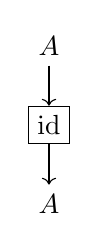
\begin{tikzpicture}
    \path
    (0,1) node(s) {$A$}
    (0,0) node[draw](id) {$\id$}
    (0,-1) node(t) {$A$}
    ;

    \draw[->] (s) -- (id);
    \draw[->] (id) -- (t);
  \end{tikzpicture}
  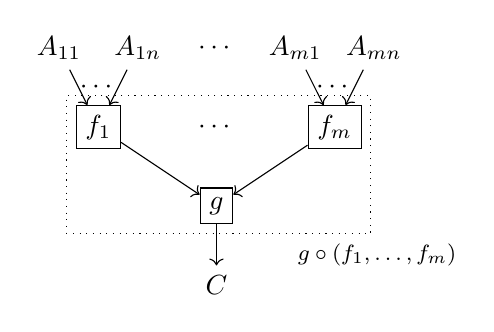
\begin{tikzpicture}
    \path
    (-2,2) node(A11) {$A_{11}$}
    (-1.5,1.5) node(A1dots) {$\cdots$}
    (-1,2) node(A1n) {$A_{1n}$}
    (0,2) node(Adots) {$\cdots$}
    (1,2) node(Am1) {$A_{m1}$}
    (1.5,1.5) node(Amdots) {$\cdots$}
    (2,2) node(Amn) {$A_{mn}$}

    (-1.5,1) node[draw](f1) {$f_1$}
    (0,1) node(fdots) {$\cdots$}
    (1.5,1) node[draw](fm) {$f_m$}

    (0,0) node[draw](g) {$g$}

    (0,-1) node(C) {$C$}
    ;

    \node[draw,dotted,fit=(f1) (fm) (g),
    label=below right:{\footnotesize$g \circ (f_1, \ldots, f_m)$}] (box) {};

    \draw[->] (A11) -- (f1);
    \draw[->] (A1n) -- (f1);
    \draw[->] (Am1) -- (fm);
    \draw[->] (Amn) -- (fm);
    \draw[->] (f1) -- (g);
    \draw[->] (fm) -- (g);
    \draw[->] (g) -- (C);
  \end{tikzpicture}

  \begin{displaymath}
    \begin{matrix}
      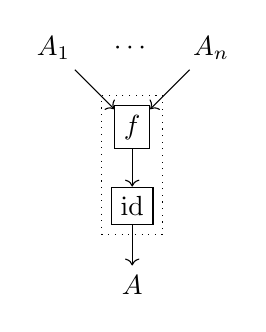
\begin{tikzpicture}[baseline]
        \path
        (-1,2) node(A1) {$A_1$}
        (0,2) node(Adots) {$\cdots$}
        (1,2) node(An) {$A_n$}
        (0,1) node[draw](f) {$f$}
        (0,0) node[draw](id) {$\id$}
        (0,-1) node(t) {$A$}
        ;

        \node[draw,dotted,fit=(f) (id)] {};

        \draw[->] (A1) -- (f);
        \draw[->] (An) -- (f);
        \draw[->] (f) -- (id);
        \draw[->] (id) -- (t);
      \end{tikzpicture}
      =
      \begin{tikzpicture}[baseline]
        \path
        (-1,1) node(A1) {$A_1$}
        (0,1) node(Adots) {$\cdots$}
        (1,1) node(An) {$A_n$}
        (0,0) node[draw](f) {$f$}
        (0,-1) node(t) {$A$}
        ;

        \draw[->] (A1) -- (f);
        \draw[->] (An) -- (f);
        \draw[->] (f) -- (t);
      \end{tikzpicture}
      &\phantom{mmmm}&
      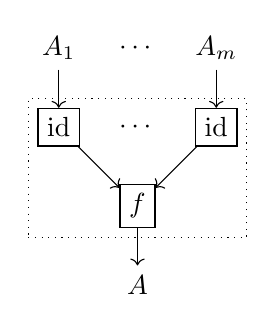
\begin{tikzpicture}[baseline]
        \path
        (-1,2) node(A1) {$A_1$}
        (0,2) node(Adots) {$\cdots$}
        (1,2) node(Am) {$A_m$}
        (-1,1) node[draw](id1) {$\id$}
        (0,1) node(iddots) {$\cdots$}
        (1,1) node[draw](idm) {$\id$}
        (0,0) node[draw](f) {$f$}
        (0,-1) node(t) {$A$}
        ;

        \node[draw,dotted,fit=(id1) (idm) (f)] {};

        \draw[->] (A1) -- (id1);
        \draw[->] (Am) -- (idm);
        \draw[->] (id1) -- (f);
        \draw[->] (idm) -- (f);
        \draw[->] (f) -- (t);
      \end{tikzpicture}
      =
      \begin{tikzpicture}[baseline]
        \path
        (-1,1) node(A1) {$A_1$}
        (0,1) node(Adots) {$\cdots$}
        (1,1) node(An) {$A_n$}
        (0,0) node[draw](f) {$f$}
        (0,-1) node(t) {$A$}
        ;

        \draw[->] (A1) -- (f);
        \draw[->] (An) -- (f);
        \draw[->] (f) -- (t);
      \end{tikzpicture}
    \end{matrix}
  \end{displaymath}

  \begin{displaymath}
    \begin{matrix}
      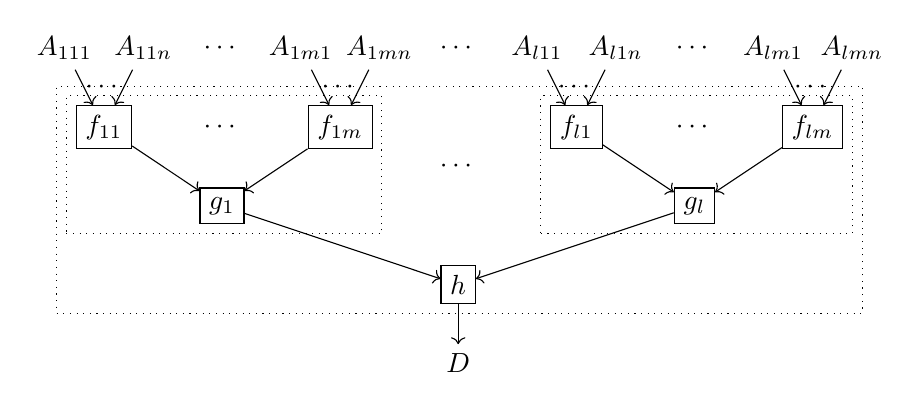
\begin{tikzpicture}
        \path
        % left
        (-5,2) node(A111) {$A_{111}$}
        (-4.5,1.5) node(A1dots) {$\cdots$}
        (-4,2) node(A11n) {$A_{11n}$}
        (-3,2) node(Adots) {$\cdots$}
        (-2,2) node(A1m1) {$A_{1m1}$}
        (-1.5,1.5) node(Amdots) {$\cdots$}
        (-1,2) node(A1mn) {$A_{1mn}$}

        (-4.5,1) node[draw](f11) {$f_{11}$}
        (-3,1) node(fdots) {$\cdots$}
        (-1.5,1) node[draw](f1m) {$f_{1m}$}

        (-3,0) node[draw](g1) {$g_1$}

        % right
        (1,2) node(Al11) {$A_{l11}$}
        (1.5,1.5) node(A1dots) {$\cdots$}
        (2,2) node(Al1n) {$A_{l1n}$}
        (3,2) node(Adots) {$\cdots$}
        (4,2) node(Alm1) {$A_{lm1}$}
        (4.5,1.5) node(Amdots) {$\cdots$}
        (5,2) node(Almn) {$A_{lmn}$}

        (1.5,1) node[draw](fl1) {$f_{l1}$}
        (3,1) node(fdots) {$\cdots$}
        (4.5,1) node[draw](flm) {$f_{lm}$}

        (3,0) node[draw](gl) {$g_l$}

        % middle
        (0,2) node {$\cdots$}
        (0,0.5) node {$\cdots$}
        (0,-1) node[draw](h) {$h$}
        (0,-2) node(D) {$D$}
        ;

        \node[draw,dotted,fit=(f11) (f1m) (g1)] (box1) {};
        \node[draw,dotted,fit=(fl1) (flm) (gl)] (boxl) {};
        \node[draw,dotted,fit=(box1) (boxl) (h)] (box) {};

        \draw[->] (A111) -- (f11);
        \draw[->] (A11n) -- (f11);
        \draw[->] (A1m1) -- (f1m);
        \draw[->] (A1mn) -- (f1m);
        \draw[->] (f11) -- (g1);
        \draw[->] (f1m) -- (g1);
        \draw[->] (g1) -- (h);

        \draw[->] (Al11) -- (fl1);
        \draw[->] (Al1n) -- (fl1);
        \draw[->] (Alm1) -- (flm);
        \draw[->] (Almn) -- (flm);
        \draw[->] (fl1) -- (gl);
        \draw[->] (flm) -- (gl);
        \draw[->] (gl) -- (h);

        \draw[->] (h) -- (D);
      \end{tikzpicture}
      \\=\\
      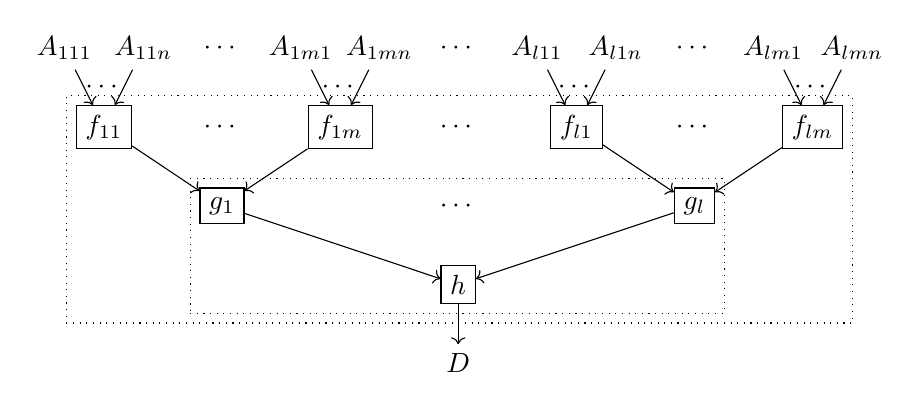
\begin{tikzpicture}
        \path
        % left
        (-5,2) node(A111) {$A_{111}$}
        (-4.5,1.5) node(A1dots) {$\cdots$}
        (-4,2) node(A11n) {$A_{11n}$}
        (-3,2) node(Adots) {$\cdots$}
        (-2,2) node(A1m1) {$A_{1m1}$}
        (-1.5,1.5) node(Amdots) {$\cdots$}
        (-1,2) node(A1mn) {$A_{1mn}$}

        (-4.5,1) node[draw](f11) {$f_{11}$}
        (-3,1) node(fdots) {$\cdots$}
        (-1.5,1) node[draw](f1m) {$f_{1m}$}

        (-3,0) node[draw](g1) {$g_1$}

        % right
        (1,2) node(Al11) {$A_{l11}$}
        (1.5,1.5) node(A1dots) {$\cdots$}
        (2,2) node(Al1n) {$A_{l1n}$}
        (3,2) node(Adots) {$\cdots$}
        (4,2) node(Alm1) {$A_{lm1}$}
        (4.5,1.5) node(Amdots) {$\cdots$}
        (5,2) node(Almn) {$A_{lmn}$}

        (1.5,1) node[draw](fl1) {$f_{l1}$}
        (3,1) node(fdots) {$\cdots$}
        (4.5,1) node[draw](flm) {$f_{lm}$}

        (3,0) node[draw](gl) {$g_l$}

        % middle
        (0,2) node {$\cdots$}
        (0,1) node {$\cdots$}
        (0,0) node {$\cdots$}
        (0,-1) node[draw](h) {$h$}
        (0,-2) node(D) {$D$}
        ;

        \node[draw,dotted,fit=(g1) (gl) (h)] (boxi) {};
        \node[draw,dotted,fit=(f11) (f1m) (fl1) (flm) (boxi)] (boxo) {};

        \draw[->] (A111) -- (f11);
        \draw[->] (A11n) -- (f11);
        \draw[->] (A1m1) -- (f1m);
        \draw[->] (A1mn) -- (f1m);
        \draw[->] (f11) -- (g1);
        \draw[->] (f1m) -- (g1);
        \draw[->] (g1) -- (h);

        \draw[->] (Al11) -- (fl1);
        \draw[->] (Al1n) -- (fl1);
        \draw[->] (Alm1) -- (flm);
        \draw[->] (Almn) -- (flm);
        \draw[->] (fl1) -- (gl);
        \draw[->] (flm) -- (gl);
        \draw[->] (gl) -- (h);

        \draw[->] (h) -- (D);
      \end{tikzpicture}
    \end{matrix}
  \end{displaymath}
\end{definition}

Multicategories have been used as a framework for reasoning with multilinear
maps in linear algebra. \todo{Reference?}
We can produce a multicategory where the objects are vector spaces, and the
multimorphisms are multilinear maps.
In this setting, we can give a universal property to the tensor product of
vector spaces.

\begin{definition}[tensor product \& tensor unit]
  Given a multicategory $\C$, a \emph{tensor product} in $\C$ is a function
  ${\otimes} : \obj\C \times \obj\C \to \obj\C$ and for each pair of objects
  $A$ and $B$, a multimorphism ${\otimes} : A, B \to A \otimes B$ such that,
  for any multimorphism $f : A, B \to C$, there is a unique way to factor $f$
  through $\otimes$, as shown below.
  Similarly, a \emph{tensor unit} is an object $I$ of $\C$ and a multimorphism
  $I : \varepsilon \to I$ supporting a nullary unique factorisation.

  \begin{tikzcd}
    A, B \arrow[rd,"f"'] \arrow[r,"\otimes"] & A \otimes B \arrow[d, dashed] \\
    & C
  \end{tikzcd}
  \begin{tikzcd}
    \varepsilon \arrow[rd,"f"'] \arrow[r,"I"] & I \arrow[d, dashed] \\
    & C
  \end{tikzcd}
\end{definition}

As the proliferation of ellipses suggests, the definition of
\emph{multicategory} I gave above is not entirely rigorous.
Indeed, mechanising the multicategory definition in a reasonably usable way is
considered an open problem. \todo{Check that no-one has done it}
However, we \emph{can} achieve a simple and usable definition in the special
case of \emph{Cartesian} multicategories.

Ordinary multicategories are to monoidal categories as Cartesian multicategories
are to Cartesian categories (i.e., categories with all finite products).
Cartesian multicategories can be defined in terms of ordinary multicategories
--- they are multicategories satisfying the usual ``structural rules'' below
and satisfying various coherence conditions on them.

\begin{align*}
  e &: \hom(\Gamma, A, B, \Delta; C) \to \hom(\Gamma, B, A, \Delta; C) \\
  w &: \hom(\Gamma; B) \to \hom(\Gamma, A; B) \\
  c &: \hom(\Gamma, A, A; B) \to \hom(\Gamma, A; B)
\end{align*}

However, we can bypass ordinary multicategories entirely, and give the following
definition inspired by our earlier formulation of intuitionistic logic.
I define Cartesian multicategories in tandem with the category of contexts and
substitutions that a Cartesian multicategory yields.

\begin{definition}
  A \emph{Cartesian multicategory} comprises the following.

  \begin{itemize}
    \item We have a collection of objects $\obj$.
          We call a list of objects a \emph{context}.
    \item For each context $\Gamma$ and object $A$, we have a set of
          (multi)morphisms $\hom(\Gamma; A)$.
          From this, we derive, for any contexts $\Gamma$ and $\Delta$, a set
          of \emph{substitutions}
          $\sub(\Gamma; \Delta) \coloneqq \prod X \in \Delta.~\hom(\Gamma; X)$.
    \item For every $i : A \in \Gamma$, we have an identity morphism
          $\id(i) : \hom(\Gamma; A)$.
          The collection of identity morphisms over $\Gamma$ serves as the
          identity substitution $\id^s : \sub(\Gamma; \Gamma)$.
    \item For substitution $\sigma : \sub(\Gamma; \Delta)$ and morphism
          $f : \hom(\Delta; A)$, we get a composite morphism
          $\sigma ; f : \hom(\Gamma; A)$.
          This allows us to compose substitutions; for
          $\sigma : \sub(\Gamma; \Delta)$ and $\tau : \sub(\Delta; \Theta)$,
          let $\sigma;^s \tau \coloneqq \lambda k.~\sigma; \tau(k)$.
    \item Identity and composition satisfy the following laws.
          \begin{itemize}
            \item $\sigma; \id(i) = \sigma(i)$
            \item $\id^s; f = f$
            \item $(\sigma;^s \tau); f = \sigma; (\tau; f)$
          \end{itemize}
          It is a simple exercise to see that these laws exactly give us the
          category laws of identity and associativity for substitutions.
  \end{itemize}
\end{definition}

The category of contexts and substitutions is furthermore Cartesian, with the
product being given by context concatenation.

\section{Weighted multicategories}
Where Cartesian multicategories give semantics to simply typed
$\lambda$-calculus, we want to find a kind of multicategories that give
semantics to $\name$.

\section{Applications}

\chapter{Semantics in worldly relations}\label{sec:wrel}

\chapter{A framework for usage-restricted calculi}\label{sec:framework}

In \cref{sec:semirings}, we saw how to use parametrisation over a partially
ordered semiring to recreate a range of usage-aware calculi.
However, $\name$, with its fixed set of type formers and syntactic forms, is a
long way from capturing the full range of linear-like programming languages
studied in the literature and required in practice.

In this chapter, I take the framework for typed syntaxes with binding developed
by \citet{AACMM21} and apply the principles we discovered in
\cref{sec:semirings} to yield a framework allowing for semiring-based usage
restrictions on variables.
Syntactically, I claim that this framework ranges over all finitiary
variable-based simply typed semiring-annotated calculi, with justification by
comparison to the framework of \citet{AACMM21} and some novel examples in
\cref{sec:other-syntaxes}.
I also derive analogues to some of the semantic results of \citet{AACMM21},
strengthening them to take advantage of usage restrictions.

The work in this chapter is fully mechanised in Agda, which allows me to be
precise about the various levels of domain-specific languages which appear.
I assume that the reader is familiar with the bunched connectives introduced in
\cref{fig:bunched} and the usage-aware environments of \cref{def:lr-env}.

\section{Syntax}

We take the insights of the previous section and use them to build a
generic framework for posemiring-annotated substructural systems in
Agda. We will first show \emph{descriptions} of systems, which are
comprised of rules that have premises combined using the bunched
combinators. We then show how to construct the Agda data type of
intrinsically well scoped, typed, and resourced terms for any given
system of our framework. We use the prototypical system from
\cref{fig:lr-comb} as a running example. \cref{sec:other-syntaxes}
presents further examples that our framework can express.

We now start to use Agda notation for record and data type
declarations, to emphasise that our framework has been implemented.

\subsection{Descriptions of Systems}

% We capture the form of rules exemplified previously\todo{Previously?} via
% \emph{descriptions} of rules.
% The key to making these descriptions work is that they only allow syntactic
% forms that preserve environments.
% These forms are: absence and multiplicity of subterms with the same usage
% annotations, absence and multiplicity of subterms with summed usage annotations,
% scaling of a subterm, and variable binding.\todo{Switching to Agda}

\paragraph{\AgdaDatatype{Premises}, \AgdaRecord{Rule}s, and \AgdaRecord{System}s.}

A type \AgdaRecord{System} is made up of multiple \AgdaRecord{Rule}s.
Each \AgdaRecord{Rule} comprises a tree of \AgdaDatatype{Premises} and
a type of conclusion. We assume that there is a
$\AgdaBound{Ty} : \AgdaPrimitiveType{Set}$ of types for the system in
scope.

The \AgdaDatatype{Premise} data type describes premises of rules,
using the bunched combinators from the previous section. A single
premise is introduced by the
\AgdaInductiveConstructor{$\langle$\_`$\vdash$\_$\rangle$}
constructor.  This allows binding of additional variables
\AgdaBound{$\Delta$} (with specified types and usage annotations) and
the specification of a conclusion type \AgdaBound{A} for this premise.
The remaining constructors are descriptions for the first-order
bunched connectives, and will be interpreted directly as such, below.

\ExecuteMetaData[\Syntaxtex]{Premises}

A \AgdaRecord{Rule} is a pair of some \AgdaDatatype{Premises} and a
conclusion. We use an infix arrow as a suggestive notation for rules.

\ExecuteMetaData[\Syntaxtex]{Rule}

Finally, a \AgdaRecord{System} consists of a set of rule labels (i.e.,
constructor names), and for each label a decsription of the
corresponding rule. We use $\rhd$ as infix notation for systems to
associate the label set with the rules.

\ExecuteMetaData[\Syntaxtex]{System}

\paragraph{\cref{fig:lr-comb} as a \AgdaRecord{System}.}

As an example, we transcribe the system defined in
\cref{fig:lr-comb} into a description.  We give the set of types of
this system as a data type \AgdaDatatype{Ty} (together with a base
type \AgdaInductiveConstructor{$\iota$}). We assume that there is a
posemiring \AgdaInductiveConstructor{Ann} in scope for the
annotations.There is one label for each instantiation of a logical
rule, but the labels contain no further information about subterms or
restrictions on the context. This will be provided when we associate
labels with \AgdaRecord{Rule}s in a \AgdaRecord{System}.

\noindent
\begin{minipage}[t]{0.5\textwidth}
  \ExecuteMetaData[\PaperExamplestex]{Ty}
  \ExecuteMetaData[\PaperExamplestex]{Side}
\end{minipage}
\begin{minipage}[t]{0.5\textwidth}
  \ExecuteMetaData[\PaperExamplestex]{qlR}
\end{minipage}

To build a system, we associate with each label a rule:

\ExecuteMetaData[\PaperExamplestex]{lR}

Compared to \cref{fig:lr-comb}, modulo the Agda notation, we can see
that the fundamental structure has been preserved: the rules match
one-to-one, and the bunched premises are the same. A major difference
is that we do not include a counterpart to the
\AgdaInductiveConstructor{var} rule in a
\AgdaRecord{System}. Variables are common to all the systems
representable in our framework.

\paragraph{Terms of a \AgdaRecord{System}.}

The next thing we want to do is to build terms in the described type system.
The following definitions are useful for talking about types indexed over
contexts, judgement forms, and judgement forms admitting newly bound variables,
respectively.

\ExecuteMetaData[\Syntaxtex]{OpenFam}

To specify the meaning of descriptions, we assume some \AgdaBound{X} : \AgdaFunction{ExtOpenFam},
% \ExecuteMetaData[\Interpretationtex]{X},
over which we form one layer of syntax, using the function
\AgdaFunction{$\llbracket$\_$\rrbracket$p} that interprets
\AgdaDatatype{Premises} defined below.  The first argument to
\AgdaBound{X} is the new variables bound by this layer of syntax, as
exemplified in the first clause of
\AgdaFunction{$\llbracket$\_$\rrbracket$p}.  The second argument is
the context containing the variables being carried over from the
previous layer.  Notice that this is not, in general, the same as the
context from the previous layer, because the usage annotations may
have been changed by connectives like
\AgdaInductiveConstructor{\_`$*$\_} and
\AgdaInductiveConstructor{\_`$\cdot$\_}.  The third argument is the
type of subterm required.

With the first clause of \AgdaFunction{$\llbracket$\_$\rrbracket$p} explained,
the rest are simply interpretations of premises into bunched combinators.

\ExecuteMetaData[\Interpretationtex]{semp}

The interpretation of a \AgdaRecord{Rule} checks that the rule targets
the desired type and then interprets the rule's premises \AgdaBound{ps}.
Notice that the interpretation of the premises is independent of the conclusion
of the rule, which accounts for the difference in type between
\AgdaFunction{$\llbracket$\_$\rrbracket$p} and
\AgdaFunction{$\llbracket$\_$\rrbracket$r}.

\ExecuteMetaData[\Interpretationtex]{semr}

The interpretation of a \AgdaRecord{System} is to choose a rule label
\AgdaBound{l} from \AgdaBound{L} and interpret the corresponding rule
\AgdaBound{rs}\AgdaSpace{}\AgdaBound{l} in the same context and for the same
conclusion.

\ExecuteMetaData[\Interpretationtex]{sems}

The most obvious way to make such an \AgdaBound{X} is to use some existing
\AgdaFunction{OpenFam} on an extended context.
We defined \AgdaFunction{Scope} to do this: take the new variables
\AgdaBound{$\Delta$}, concatenate them onto the existing context
\AgdaBound{$\Gamma$}, and pass the extended context onto the judgement
\AgdaBound{T}.

\ExecuteMetaData[\Syntaxtex]{Scope}

%{\color{red}(Forward ref: for now, we could have inlined \texttt{Scope}.)}

We use \AgdaFunction{Scope} to deal with new variables in syntax.
Terms resemble the free monad over a layer-of-syntax functor, though
that picture is complicated by variable binding.  A term is either a
variable or a use of a logical rule together with terms for each of
the required subterms. The \AgdaFunction{Size} argument is where we
use sized types to convince Agda that this type is strictly positive.

\ExecuteMetaData[\Termtex]{Term}

Terms defined like this are still quite difficult to write, mainly because of
frequently changing usage contexts and the need for proofs that they all match
up.
We will see how to automate these proofs in \cref{sec:usage-elaborator}.

%Here is an example term, using the \AgdaFunction{$\lambda$R} system.
%First, for ease of writing, we introduce pattern synonyms for each of the
%typing rules we use.

%\ExecuteMetaData[\PaperExamplestex]{patterns}

%Our example term is a function that flips a tagged union wrapped in an
%arbitrarily annotated \emph{bang}.
%Much of the effort in writing such a term goes into writing the various
%relatedness proofs between usage contexts --- observing, for example, that two
%usage contexts sum together to make a third, or that a usage context used for
%a variable is a basis vector.
%We give a method of automating these proofs in \cref{sec:usage-elaborator}.
%\todo{To be clear, we don't actually write this.}

%\ExecuteMetaData[\HeavyItex]{lR-term}

% A layer of syntax supports the following functorial action.

% \ExecuteMetaData[\Maptex]{map-s-type}

\subsection{Other syntaxes and syntactic forms}\label{sec:other-syntaxes}

\paragraph{The system $\mu\tilde\mu$.}
We can encode a usage-annotated version of System $L$/the
$\mu\tilde\mu$-calculus~\cite{CH00} --- a syntax for classical logic --- in
such a way that contexts capture the undistinguished parts of the sequent.
As such, the generic substitution lemma we get in \cref{sec:kits} is the form
of substitution required in standard $\mu\tilde\mu$-calculus metatheory.
Though the $\mu\tilde\mu$-calculus is originally described as a sequent
calculus~\cite{CH00}, we use the techniques of
\citet[p.~12]{herbelin-hab} and \citet{LC06} to present it as a natural
deduction system, thus giving a notion of \emph{variable} to the system.

Unlike the single judgement form of \name{} and standard simply typed
$\lambda$-calculi, the $\mu\tilde\mu$-calculus has three judgement forms:
terms, coterms, and commands.
Read logically, terms and coterms are seen to, respectively, prove and refute
propositions (types), while commands exhibit contradictions.
This means that the abstract \AgdaBound{Ty} in the generic framework is
instantiated to \AgdaDatatype{Conc} (for \emph{conclusion}) as below, with
\AgdaDatatype{Ty} not being exposed directly to the generic framework.
For now, we just consider multiplicative disjunction $\parr$ (\emph{par}) and
negation/duality, beside an uninterpreted base type.
These are enough to exhibit classical behaviour.

\noindent
\begin{minipage}[t]{0.5\textwidth}
  \ExecuteMetaData[\MuMuTildetex]{Ty}
\end{minipage}
\begin{minipage}[t]{0.5\textwidth}
  \ExecuteMetaData[\MuMuTildetex]{Conc}
\end{minipage}

With \AgdaBound{Ty} instantiated as \AgdaDatatype{Conc}, all terms are assigned
\AgdaDatatype{Conc} type, as are all the variables.
No variables are given \AgdaInductiveConstructor{com} type, similar to how in
the bidirectional typing syntax of \citet[p.~25]{AACMM21}, no variables are
given \AgdaInductiveConstructor{Check} type.
How to observe this invariant is covered in the latter paper, so we will not
repeat it here (having not yet seen how to write traverals on terms).

The syntax comprises a \emph{cut} between a term and a coterm of the same type,
the eponymous $\mu$ and $\tilde\mu$ constructs for proof by contradiction, and
then term and coterm (introduction and elimination) forms for negation and
\emph{par}.

\ExecuteMetaData[\MuMuTildetex]{MMT}

%With a collection of pattern synonyms and the machinery from
%\cref{sec:usage-elaborator}, we can write an example term: a function which
%flips the disjuncts of a \emph{par}.

%\ExecuteMetaData[\MuMuTildeTermtex]{patterns}
%\ExecuteMetaData[\MuMuTildeTermtex]{myComm}

\paragraph{Duplicability}
There is one more bunched combinator we have experimented with adding to the
framework:

\[
  \plr{\Box T}\,\grR \coloneqq \Sigma\grRprime.~\plr{\grRprime \leq \grR}
  \times \plr{\grRprime \leq \gr0}
  \times \plr{\grRprime \leq \grRprime + \grRprime}
  \times T\,\grRprime
\]

The idea of $\plr{\Box T}\,\grR$ is to assert that $\grR$, or some refinement
of it, can be both discarded and duplicated indefinitely, and in the
refinement we have a $T$.
We use this combinator to introduce subterms that are used an unknown number of
times, for example the continuations of the eliminator of an inductive type,
or other fixed points.
We can also use it in linear/non-linear style systems~\cite{Benton94} to make
sure linear variables are not available in the intuitionistic fragment.

Adding the $\Box$ combinator is the only thing we have found that requires our
linear maps be functional rather than merely relational.


\section{Semantics}

Given a $\V$-environment $\Gamma \Rightarrow \Delta$, the function
\AgdaFunction{semantics} we define in this section assigns a
$\C$-value in context $\Gamma$ to every term in context $\Delta$,
where $\C$ is an \AgdaFunction{OpenFam} being the carrier of the
semantic interpretation of terms ($\V$ being the semantic
interpretation of variables). Before we can define
\AgdaFunction{semantics}, we need to treat recursion through rules'
premises (\cref{sec:functorial}) and extension of environments when
going under variable binders (\cref{sec:kripke}).
\todo{Maybe split the chapter here. Syntax/semantics}

% Our goal in this section is to define \AgdaFunction{semantics}, a
% recursor that turns a term into a \AgdaBound{$\C$}-value using a
% \AgdaBound{$\V$}-environment, in a type preserving way:\bob{Get rid of
%   ``body'' here}

% \ExecuteMetaData[\Semanticstex]{semantics-type}

% The \AgdaBound{$\V$} and \AgdaBound{$\C$} are \AgdaFunction{OpenFam}s,
% representing the interpretations of variables and terms
% respectively. In \cref{sec:traversal} we will see the data that must
% be provided to make a \AgdaFunction{semantics} for a given
% system. Before that, we must see how to deal with the two complicated
% features of our syntax: the usage annotations (\cref{sec:functorial})
% and variable binding (\cref{sec:kripke}). \todo{fwd ref to where these are used}

\subsection{A layer of syntax is functorial}\label{sec:functorial}

A basic property of the universe of syntaxes we described in \cref{sec:syntax}
is that every syntax supports a functorial action on subterms, realised by the function \AgdaFunction{map-s}.
Its type says that to map a function \AgdaBound{f}
over a layer of syntax, there must be a linear map \AgdaBound{F} relating the
domain and codomain usage contexts, and \AgdaBound{f} should be usable
wherever the domain and codomain usage contexts are similarly related by
\AgdaBound{F}.

\ExecuteMetaData[\Maptex]{map-s-type}

This generality is needed because usage contexts change between
a term and its immediate subterms---they are decomposed according to the bunched connectives used in the rules.
\AgdaBound{X} and \AgdaBound{Y} are \AgdaFunction{ExtOpenFam}s, with
\AgdaBound{$\Theta$} being the context extension for a subterm (i.e., the
variables newly bound in that subterm).
Unlike usage annotations, types in the contexts \AgdaBound{$\gamma$} and \AgdaBound{$\delta$}, and the conclusion types implicit here, are preserved throughout.
This is the essence of the usage annotation based approach---we use traditional techniques for variable binding, with the usage annotations layered on top.

The heart of \AgdaFunction{map-s} is \AgdaFunction{map-p}, which recursively
works through the structure \AgdaBound{ps} of premises of the rule applied,
acting on each subterm it finds.
Here, particularly in the clauses for \AgdaInductiveConstructor{`$\sep$} and
\AgdaInductiveConstructor{`$\cdot$}, we see why it is not enough for the
function on subterms to apply at usage contexts \AgdaBound{P} and \AgdaBound{Q}
--- rather, it also needs to apply at any similarly related \AgdaBound{P$'$}
and \AgdaBound{Q$'$}.
In the case of \AgdaInductiveConstructor{`$\sep$}, we have that
$\grP \leq \grP_M + \grP_N$, with \AgdaBound{M} and \AgdaBound{N} being
collections of subterms in usage contexts $\grP_M$ and $\grP_N$, respectively.
Linearity of \AgdaBound{F} yields $\grQ_M$ and $\grQ_N$ such that
$\grQ \leq \grQ_M + \grQ_N$ and we use \AgdaFunction{map-p} recursively at
$(\grP_M, \grQ_M)$ and $(\grP_N, \grQ_N)$ on \AgdaBound{M} and \AgdaBound{N}.
The cases for \AgdaInductiveConstructor{`$\cdot$} and
\AgdaInductiveConstructor{`$I^*$} are similar, each using a different aspect
of linearity.
In contrast, the cases for \AgdaInductiveConstructor{`$\dot1$} and
\AgdaInductiveConstructor{`$\dot\times$}, which are the only constructors used in fully structural
systems, do not involve any changes in the usage contexts.

\ExecuteMetaData[\Maptex]{map-p}

\subsection{The Kripke function space}\label{sec:kripke}

At this point we introduce a minor generalisation to
\AgdaFunction{OpenFam} and \AgdaFunction{ExtOpenFam}:
\AgdaBound{I}\AgdaSpace{}\AgdaFunction{---OpenFam} and
\AgdaBound{I}\AgdaSpace{}\AgdaFunction{---ExtOpenFam}.  We obtain the
definition of \AgdaBound{I}\AgdaSpace{}\AgdaFunction{---OpenFam} by
replacing the textual occurrence of \AgdaBound{Ty} by the parameter
\AgdaBound{I}.

The definition \AgdaFunction{Kripke}\,$\V$\,$\C$\,$\Delta$ is a kind
of function space that describes a $\C$ value parametrised by
$\Delta$-many additional $\V$s (all correctly typed and usage
annotated). It is used to describe how to go under binders in a
Higher-Order Abstract Syntax style---to go under a binder we must
provide semantic interpretations for all the additional variables:

% When going under binders during a recursion, the context will be extended by some $\Theta$. This means that the current environment must be extended with $\Theta$s-worth of $\V$s

% we need the ability to say that

% Kripke V C is given the extension \Theta

% In \cref{sec:terms}, we defined \AgdaFunction{Scope} to let a
% judgement-indexed family admit context extensions. However, a key
% component of our generic semantic traversal is to make use of the open
% family \AgdaBound{$\V$} of \emph{values}, which are the sort of thing
% we store in an environment.  The definition \AgdaFunction{Kripke}
% gives an alternative to \AgdaFunction{Scope} which interprets the
% newly bound variables via a requirement of $\V$-values rather than
% extra assumptions for the $\C$-computation.

\ExecuteMetaData[\Semanticstex]{Kripke}

\AgdaFunction{Wrap}
is a device that turns any type family into an equivalent type family
that is judgementally injective in its indices, which helps with
Agda's type inference.
It turns the type family into a parametrised
record with a single field \AgdaField{get} whose type is the type in
the body of the $\lambda$-abstraction.
For understanding the meaning of
\AgdaFunction{Kripke}, \AgdaFunction{Wrap} can be ignored.

If $\Delta$ is of the form $\gr{s_1}B_1, \ldots, \gr{s_n}B_n$, then
\ExecuteMetaData[\Snippetstex]{KripkeVCDGA}\ is equivalent to
\ExecuteMetaData[\Snippetstex]{KripkeExpanded}\ by Currying.  That is
to say, the Kripke function is expecting a value for each newly bound
variable, at the multiplicity of its annotation, together with the
resources supporting each of those values. We use the ``magic wand''
function space here to enforce the invariant that the freshly bound
variables have usage annotations that are added to the existing
variables, not shared with them. The use of the
\AgdaFunction{$\Box^r$} modality ensures that we can still use it in
the presence of additional variables introduced by weakening.

\AgdaFunction{Kripke} is functorial in the \AgdaBound{$\C$} argument,
as witnessed by the \AgdaFunction{mapK$\C$} function, which is essentially
post-composition:

\ExecuteMetaData[\Semanticstex]{mapKC}

% is exemplified by the following construct
% \AgdaFunction{reify}, where we weaken \AgdaBound{$\Gamma$} by a $\gr0$ed-out
% version of \AgdaBound{$\Delta$}.
% The \AgdaBound{$\Delta$} then gets filled in by the $\V$-values.

% \bob{Move this para}
% This means that \AgdaBound{A} in the definition of \AgdaFunction{Kripke} has
% type \AgdaBound{I}, rather than specifically \AgdaBound{Ty}.
% We use this generality later in \AgdaFunction{extend}, setting \AgdaBound{I}
% to \AgdaDatatype{Ctx}.

\subsection{Semantic traversal}\label{sec:traversal}

We can now state the data required to implement a traversal assigning
semantics to terms. For open families $\V$ and $\C$, interpreting
variables and terms respectively, we assume that $\V$ is renameable,
that $\V$ is embeddable in $\C$, and that we have an algebra for a
layer of syntax, where bound variables are handled using the Kripke
function space:

% The aim of this subsection is to give an alternative recursion principle for
% terms that incorporates some of the environment-handling seen in the
% implementations of renaming and substitution.
% The rest of this section assumes the following: a renameable open family
% \AgdaBound{$\V$} that embeds into the open family \AgdaBound{$\C$}, and an
% algebra for a layer of syntax at \AgdaBound{$\C$}.

\ExecuteMetaData[\Semanticstex]{Semantics}

%\ExecuteMetaData[\Semanticstex]{Comp}

We mutually define the action \AgdaFunction{semantics} and its lemma
\AgdaFunction{body}.
The purpose of \AgdaFunction{semantics} is to turn a term into a
\AgdaBound{$\C$}-value using a \AgdaBound{$\V$}-environment and the fields of
\AgdaRecord{Semantics}.
Meanwhile, \AgdaFunction{body} does a similar job, but also deals with
newly bound variables.
In particular, \AgdaFunction{body} takes a term in a context extended by
\AgdaBound{$\Theta$}, and produces a Kripke function from
\AgdaBound{$\V$}-values for \AgdaBound{$\Theta$} to \AgdaBound{$\C$}-values.

\ExecuteMetaData[\Semanticstex]{semantics-type}

To implement the new recursor \AgdaFunction{semantics}, we use the standard
recursor, which in one case gives us a variable \AgdaBound{v}, and in the other
gives us a structure of subterms \AgdaBound{M}, each of which is in an extended
context.
To deal with a variable \AgdaBound{v}, we look it
up in the environment \AgdaBound{$\rho$}, then use the
\AgdaField{$\sem{\text{var}}$} field to map the resulting
\AgdaBound{$\V$}-value to a \AgdaBound{$\C$}-value.
To deal with a structure of subterms \AgdaBound{M}, we use the functoriality of
the syntactic structure to consider each subterm separately.
On a subterm, we apply \AgdaFunction{body}, which amounts to a recursive call
to \AgdaFunction{semantics} with an extended environment.
Recall that \AgdaFunction{relocate} (\cref{thm:env-resize}) adjusts the
environment \AgdaBound{$\rho$} to work in the usage contexts of the subterms.

\ExecuteMetaData[\Semanticstex]{semantics}

For \AgdaFunction{body}, we are given a subterm \AgdaBound{M}, to
which we want to apply \AgdaFunction{semantics}.  To do so, we need an
extended version of the initial environment \AgdaBound{$\rho$}. We
express this as the generation of a Kripke function that produces the
extended environment given interpretations of the fresh variables. We
take \AgdaBound{$\rho$}, which is an environment covering
\AgdaBound{$\Delta$}, and \AgdaBound{$\sigma$}, which is an
environment covering \AgdaBound{$\Theta$}, and glue them together
using the inductive rules for generating environments, after having
renamed \AgdaBound{$\rho$} via \cref{thm:env-ren} to make it fit the
new context \AgdaBound{$\Gamma^+$} (intended to be
\ExecuteMetaData[\Snippetstex]{GT}):

\ExecuteMetaData[\Semanticstex]{extend}

% The best we can achieve without identity environments for \AgdaBound{$\V$} is
% a Kripke function returning an extended environment.
To define \AgdaFunction{body}, we use \AgdaFunction{mapK$\C$} to
post-compose the environment extension by the
\AgdaSymbol{$\lambda$}-function taking an extended environment and
acting with it on \AgdaBound{M}.

\ExecuteMetaData[\Semanticstex]{body}

% \todo{FIX} Under the assumption that \AgdaBound{$\V$} is renameable, we can decompose
% \cref{thm:lr-bind} as
% \AgdaFunction{reify}\AgdaSpace{}\AgdaOperator{\AgdaFunction{$\circ$}}%
% \AgdaSpace{}\AgdaFunction{extend}, with \AgdaFunction{extend} defined below.
% We can think of \AgdaFunction{extend} as our best effort to extend an
% environment by \AgdaBound{$\Theta$} without access to an identity environment
% at \AgdaBound{$\Theta$}.


\section{Example semantics}\label{sec:example-semantics}

\subsection{Renaming and substitution}\label{sec:kits}

In an unpublished note, \citet{McBride05} gives a parametrised traversal
yielding homomorphisms of syntax.
The parameters are collected in the record \AgdaRecord{Kit}.
We make a minor change to the original presentation, where instead of our
\AgdaField{ren\textasciicircum{}$\V$} field, \citeauthor{McBride05} has the
field \AgdaField{wk} allowing only context extensions.
As for the other two fields, \AgdaField{vr} allows us to map variables to
$\V$-values, so as to put newly bound variables in environments; and
\AgdaField{tm} allows us to extract terms from $\V$-values, as required when
we use the environment to evaluate a free variable.

\ExecuteMetaData[\Syntactictex]{Kit}

Where \citeauthor{McBride05} gave the traversal explicitly, we go via our
generic semantic traversal.
The first two fields of \AgdaRecord{Semantics} derive directly from fields of
\AgdaRecord{Kit}.
Meanwhile, to handle term constructors, we first \AgdaFunction{reify} to get a
collection of traversed subterms, and then use \AgdaInductiveConstructor{`con}
to assemble these subterms into a similarly shaped syntactic form as we started
with.
The \AgdaField{vr} field is used implicitly in \AgdaFunction{reify}, as it is
used to show that $\V$-identity environments exist.

\ExecuteMetaData[\Syntactictex]{kit-to-sem}

The action of a syntactic traversal on logical rules is basically fixed: we
preserve the logical rule and extend the environment with any newly bound
variables according to \AgdaField{vr}.
Meanwhile, the action on variables is relatively unconstrained: we look up the
variable in the environment to get a $\V$-value, then transform that $\V$-value
into a term using \AgdaField{tm}.

The idea of renaming is that variables replace variables, whereas with
substitution, terms replace variables.
This translates to environments for renaming containing $\sqni$-values
(variables), and environments for substitution containing $\vdash$-values
(terms).

%To implement renaming and substitution for terms, we now just implement
%syntactic kits for variables and terms, respectively.

\ExecuteMetaData[\Syntactictex]{Ren-Kit}

Notice that \AgdaFunction{ren\textasciicircum$\vdash$}, witnessing the fact
that terms are renameable, is a corollary of \AgdaFunction{Ren-Kit}.

\ExecuteMetaData[\Syntactictex]{Sub-Kit}

\subsection{A denotational semantics}

\todo{Introduction}
To abbreviate this section, we use a simplified syntax compared to \name{}.
We allow for an arbitrary family of base types \AgdaBound{BaseTy}, and a single
type former \mbox{\ExecuteMetaData[\WReltex]{rAToB}}, equivalent to
\mbox{\ExecuteMetaData[\PaperExamplestex]{BangrAToB}} from the earlier system.

\ExecuteMetaData[\WReltex]{Ty}

In the term syntax, $\lambda$-abstraction now binds a variable with annotation
\AgdaBound{r}, while application needs to scale its argument by \AgdaBound{r}
(both in accordance with the function type they are acting on).

\ExecuteMetaData[\WReltex]{AnnArr}

In this subsection, we take the usage annotations to be the 4-element variance
posemiring.
\todo{This works for any semiring.}
We establish the property that all terms are monotonic in their free variables.
This monotonicity can be covariant or contravariant (or neither or both)
depending on the annotation of each free variable.
This provides an additional example to those of \citet{AbelBernardy2020}.
\todo{Cite before here.}

We will take semantics of this system into
\emph{worldly relations}~\cite{AbelBernardy2020}.
A worldly relation over a poset of worlds \AgdaBound{W} is a set over which
we have a \AgdaBound{W}-indexed binary relation satisfying a presheaf-like
property with respect to the order on \AgdaBound{W}.

\ExecuteMetaData[\WReltex]{WRel}

\begin{example}
  When \AgdaBound{W} is the 1-element set, a worldly relation is just a set
  equipped with a binary relation.
\end{example}

Morphisms between worldly relations \AgdaBound{R} and \AgdaBound{S} consist of
a mapping between the underlying sets such that that mapping preserves
relatedness from \AgdaBound{R} to \AgdaBound{S}.

\ExecuteMetaData[\WReltex]{WRelMor}

\todo{Define big intersection.}
When the poset of worlds forms a (relational) commutative monoid, such worldly
relations support a symmetric monoidal closed structure.
We reuse the bunched connectives \AgdaRecord{$I^*$}, \AgdaRecord{$\sep$}, and
\AgdaRecord{$\wand$}, now over worlds rather than contexts.

\ExecuteMetaData[\WReltex]{IR}
\ExecuteMetaData[\WReltex]{tensorR}
\ExecuteMetaData[\WReltex]{lollyR}

The final piece of sematics we need is a \emph{bang} operator.
\todo{No instead}
Instead of requiring extra algebraic structure on the worlds, we allow the
semantic \emph{bang} to be an arbitrary annotation-indexed functor on worldly
relations.
This functor must respect all of the structure on the indices, making it a
graded comonad over multiplication, as well as being lax monoidal at any
particular index \AgdaBound{r}.

\ExecuteMetaData[\WReltex]{Bang}

\begin{example}
  With \AgdaBound{W} being the 1-element set and annotations coming from the
  variance semiring, we can define the following \emph{bang}.
  It is always the identity on the set component, while the relation component
  consists of flipping the relation for contravariance and taking conjunctions
  to achieve both covariance and contravariance.
  When we want neither covariance nor contravariance, we use the always true
  predicate on worlds \AgdaFunction{$\dot1$}.

  \ExecuteMetaData[\Monotonicitytex]{BangR}
\end{example}

To associate semantics to syntax, we start as standard by associating worldly
relations to types.
We also extend the semantics of types to contexts, using \AgdaFunction{I$^R$},
\AgdaFunction{$\otimes^R$}, and \AgdaField{!$^R$} to interpret the empty
context, concatenation, and usage annotations on singletons, respectively.

\ExecuteMetaData[\WReltex]{sem}

The semantics of a term is then to be a morphism from the interpretation of the
context to the interpretation of the term's type.

\ExecuteMetaData[\WReltex]{sem-vdash}

Variables are given semantics by \AgdaFunction{lookup$^R$} (definition omitted).

\ExecuteMetaData[\WReltex]{lookupR-type}

Now, we give a \AgdaRecord{Semantics}.
The choice of \AgdaBound{$\V$} as
\AgdaRecord{\AgdaUnderscore{}$\sqni$\AgdaUnderscore{}} is somewhat arbitrary,
given that a standard denotational semantics would not use intermediate
environments in the same sense as renaming and substitution, but allows us to
reuse the standard facts that variables support renaming and identity
environments.
With this choice of \AgdaBound{$\V$} and \AgdaBound{$\C$}, we interpret
environment entries by \AgdaFunction{lookup$^R$}.
Meanwhile, for the logical rules, we ignore environments by using
\AgdaFunction{reify} to just deal with morphisms in an extended context.
As such, $\lambda$-abstractions are easy to interpret, while applications
require some massaging to remove the extension by an empty context, followed by
some plumbing to split the interpretation of the context according to the usage
constraints and feed the interpretation of the argument \AgdaBound{n$'$} into
the interpretation of the function \AgdaBound{m$'$}.

\ExecuteMetaData[\WReltex]{Wrel}

In order to map open terms to interpretations, we take the action of the
semantics and give the identity renaming as the starting environment.

\ExecuteMetaData[\WReltex]{wrel}

\begin{example}
  We can make a subtraction function from primitive addition and negation on
  integers.
  Subtraction is covariant in its first argument and contravariant in its
  second argument.
  We give the definition in pseudocode, as we have not yet seen how to
  conveniently write terms (\cref{sec:usage-elaborator}).

  \begin{align*}
    &{\sim\sim}p :
      {\uparrow\uparrow}\mathbb Z \multimap
      {\uparrow\uparrow}\mathbb Z \multimap \mathbb Z,
      {\sim\sim}n : {\downarrow\downarrow}\mathbb Z \multimap \mathbb Z
      \vdash \mathnormal{minus} :
      {\uparrow\uparrow}\mathbb Z \multimap
      {\downarrow\downarrow}\mathbb Z \multimap
      \mathbb Z
    \\
    &\mathnormal{minus} \coloneqq \lambda x.~\lambda y.~p\,x\,(n\,y)
  \end{align*}

  We observe that the set component of this term's semantics is just the
  expected Agda function when the two free variables are given appropriate
  interpretations.

  \ExecuteMetaData[\Monotonicitytex]{minus-set}

  Furthermore, the relational component of the semantics yields the free
  theorem that the Agda subtraction so defined is monotonic in the expected way.
  This relies on library proofs that addition and negation are suitably
  monotonic.

  \ExecuteMetaData[\Monotonicitytex]{thm}
\end{example}

\subsection{A usage elaborator}\label{sec:usage-elaborator}

Using the constructs we have seen so far, producing example terms soon becomes
extremely tedious.
We achieved some abbreviation by using pattern synonyms, but we still have to
produce essentially bespoke proofs whenever we use a usage-sensitive part of the
syntax.
The size of each of these proofs is roughly proportional to the number of free
variables, so the amount of proof we have to write grows roughly quadratically
with the size of terms.
An additional factor, which we can't see on paper, is that type checking time
for these proofs soon becomes prohibitive to interactive development.

Our aim in this subsection is to automate usage constraint proofs, making terms
both easier to write and more performant to check.
We invoke the automation by writing terms in a syntax where usage constraints
have been trivialised, and then use a semantic traversal over the simplified
syntax to try to produce a fully elaborated term in the original syntax.
We write the automation in a way that is generic in the syntax description, thus
avoiding repetition and facilitating the prototyping of new type systems.

The type of syntax descriptions depends on the type of usage annotations because
of variable binding.
For example, in the $\oc_{\gr r}$-E rule of \cref{fig:lr-comb}, the right
premise binds a new variable with annotation $\gr r$, where $\gr r$ is drawn
from the ambient posemiring.
The scaling combinator also makes direct reference to the posemiring.
To produce a simplified syntax description, where usage constraints are
trivialised, we set the ambient posemiring to the 1-element $\mathbf0$
posemiring.
In contrast to syntax descriptions, even though types can contain usage
annotations, the type of types does not depend on the type of usage annotations.
This means that, in our simplified syntax, terms have types from the original
system even though variables have trivial usage annotations.
We define the $\mathbf0$ posemiring as follows, being careful to use the
0-field record type \AgdaRecord{$\top$} so that everything algebraic gets
solved by Agda's $\eta$-laws.
Indeed, in this very definition, all of the semiring operations and laws are
canonically inferred.

\ExecuteMetaData[\UsageChecktex]{0-poSemiring}

The elaboration process is monadic.
In particular, we use the \AgdaDatatype{List}/non-determinism monad to give
\emph{all} of the possible annotation choices on the free variables of a term.
We believe the commitment to multiple solutions is inherent when the syntax
contains \AgdaInductiveConstructor{`$\dot1$}.
For example, in the intermediate stages of elaborating
$\plr{\vdash \lambda x.~\plr{*,*}} : A \multimap \top \otimes \top$ with a
usage counting posemiring (assuming reasonable rules for $\top$ and $\otimes$),
it is unclear whether to use the variable $x$ in the left $*$ or the right $*$.
This uncertainty should be reflected in the final result.

The non-deterministic choices we make during elaboration are enumerated by
the fields of \AgdaRecord{NonDetInverses}.
These choices are driven by the typing rules and a candidate usage vector for
the conclusion.
For example, \AgdaField{+$^{-1}$}\AgdaSpace{}\AgdaBound{r} is needed when we
encounter a \AgdaInductiveConstructor{`$\sep$} in the syntax and the candidate
usage annotation we are considering is \AgdaBound{r}.
Then, \AgdaField{+$^{-1}$}\AgdaSpace{}\AgdaBound{r} is a list of pairs of
annotations \AgdaBound{p} and \AgdaBound{q} that \AgdaBound{r} can split into,
together with a proof of the splitting.
For \AgdaField{0\#$^{-1}$} and \AgdaField{1\#$^{-1}$}, inverses to constants,
we are given the candidate \AgdaBound{r} and typically return an empty list if
the constraint cannot be satisfied, or a singleton list containing a proof.
\AgdaField{*$^{-1}$} is used when we encounter scaling, in which case we know
both the scaling factor \AgdaBound{r} (from the syntax description) and the
candidate \AgdaBound{q}.
These inverse operations combine monadically (in fact, applicatively) to give
inverses to the vector operations of zero, addition, scaling, and basis.

\ExecuteMetaData[\UsageChecktex]{NonDetInverses}

We choose the \AgdaBound{$\V$} of our semantics to be (unannotated) variables.
For the \AgdaBound{$\C$}, we consider \emph{functions} from candidate usage
vectors \AgdaBound{R} to the list of elaborated derivations with usage
annotations given by \AgdaBound{R}.
The module name \AgdaModule{U} refers to the fact that we are taking the
ambient posemiring to be $\mathbf0$ in \AgdaFunction{OpenFam}.
The effect on \AgdaFunction{OpenFam} is that the usage annotations of any
contexts we consider are uninformative (hence the \AgdaSymbol{\_} on the left).

\ExecuteMetaData[\UsageChecktex]{C}

To traverse the unannotated terms, we produce a \AgdaRecord{Semantics} over the
unannotated system \AgdaFunction{uSystem}\AgdaSpace{}\AgdaBound{sys}.
We already know that variables are renameable.
To interpret a variable, we consider all the possible proofs that such a
variable could be well annotated, and package them up as a variable term.

\ExecuteMetaData[\UsageChecktex]{elab-sem}

\ExecuteMetaData[\UsageChecktex]{lemma-type}

To actually use \AgdaFunction{elab-sem} on terms, we take the associated
\AgdaFunction{semantics} and pass it the identity environment (an identity
\emph{renaming} in this case, because $\V$ is a family of variables).
The candidate usage vector \AgdaBound{R} will be empty for closed terms, and
otherwise we have to supply the intended usage annotations.


\chapter{Conclusions}\label{sec:conc}

In this thesis, I have developed a foundation for semiring-annotated calculi
presented in natural deduction style.
I have given a consolidated account of the semiring-annotated calculus $\name$,
including its relations to existing linear and modal calculi.
As part of this, I have adapted what I call \emph{bunched connectives} from
\cite{RPKV20} as a way to state the typing rules of the calculus as well as to
work with the metatheory.
The distinction between sharing and separating conjunction given by the bunched
connectives corresponds well to the notions of \emph{additive} and
\emph{multiplicative} connectives in the object language, respectively.
Following this, I have given a novel linear algebra-based definition of
\emph{environment} for semiring-annotated calculi, together with a motivation
which may serve as a basis for the corresponding definition for other
substructural systems.
The adequacy of this definition of environment is shown by my implementation of
simultaneous renaming and substitution, as well as other operations on
environments, like composition of renamings and substitutions.

With the details of $\name$ worked out, I then moved on to adapting the work of
\citet{AACMM21} so as to make it able to capture semiring-based usage
restrictions, as found in $\name$.
The syntax descriptions of the resulting system are based on the bunched
connectives, and are shown to be expressive enough to encode calculi of a
variety of forms.
In adapting the semantics, I am forced to be precise about \emph{sharing} and
\emph{separating} bunched connectives, but largely add these as a refinement of
the work of \citet{AACMM21}.
I provide the renaming and substitution operations for all expressible calculi.
I also provide more specialised examples of semantic traversals:
a usage elaborator, an NbE algorithm, a denotational semantics, and translations
between different calculi.
The usage elaborator gives an unexpected example of generic programming, which
one could not write without syntax descriptions.
% Other examples...
Together, these examples show the applicability and versatility of the framework
I have developed.

FIXME: the next two paragraphs are directly from the ESOP22 paper.

We have presented a framework for doing metatheory for a class of substructural
type systems in Agda.
The framework gives us renaming, substitution, and a usage elaborator for new
syntaxes for free, which we hope can facilitate prototyping and the
mechanisation of more interesting semantic results.
Beside the mechanised framework itself, we believe its methodology --- the use
of bunched premise combinators --- can guide and simplify the development of
(potentially unmechanised) substructural type systems.

Our account of substructurality is based on the linear algebraic
principles described by \citet{WA21}.
However, these details only really affect the definition of environment,
in which the use of linear maps is motivated by them being the standard notion
of morphism between vectors.
We could imagine that a similar notion of morphism is found for the kind of
annotations found in \citet{LicataSR17}, allowing a framework to consider
finer substructural systems.

\begin{itemize}
  \item Novel simultaneous substitution for linear type theories
  \item Generalise \citet{AACMM21} work to substructural logics
  \item Is this a reusable library? Yes, examples
  \item Methodology for metatheory of new calculi
  \item Semirings have been a reasonably robust basis.
  \item Can the code be directly generalised?
    Abstract away the algebraic structure of contexts.
\end{itemize}

\section{Future work}

\begin{itemize}
  \item Fitch-style systems (can't do).
\end{itemize}

\subsection{Further work}

\paragraph{Equality}
Perhaps the most fundamental missing piece from the metatheoretic account of
semiring-annotated calculi I have given in this thesis is equations between
terms.
Reasoning about equality between terms and environments is a problem I have
tried to solve, but I have not arrived at a satisfactory solution in the time
available to me.

I believe that the basic difficulty of giving an account for equality in a
linear setting is the proliferation of $\Sigma$-types.
For example, describing equality between two applications of
\TirName{$\with$-I} is immediate: $\Gamma \vdash (M, N) = (M', N') : A \with B$
if and only if $\Gamma \vdash M = M' : A$ and $\Gamma \vdash N = N' : B$.
However, to do the same with \TirName{$\otimes$-I} requires us to be careful
about the contexts of the subterms.
The two applications of \TirName{$\otimes$-I} may a priori split the context in
different ways, and should only be equated when those splittings are equal
(in the appropriate sense).
If the splittings are equal, then the contexts of the subterms will line up, and
only then can the subterms themselves be compared for equality.
These multiple stages come about because $\plr{T * U}\,\Gamma$ is a
$\Sigma$-type, and equality of elements of $\Sigma$-types always follows this
pattern.
Such reasoning becomes even more complex for environments, which are equivalent
to iterated $*$-families.
Additionally, it is unclear what effect subsumption of contexts (like subusaging
in this thesis or explicit structural rules in other calculi) should have on
equality, particularly when the subsumption commutes with parts of the subterms.

Previous work on linear logic has preferred to deal with equations only on
untyped terms. \todo{Check this.}

\paragraph{Polymorphism}
An important feature of most contemporary statically typed programming languages
is polymorphism.
In particular, parametric polymorphism over types can be used to significantly
improve code reuse, and is well undestood theoretically via System $F$ and its
variants.
I have not considered polymorphism in this thesis, and neither did
\citet{AACMM21} in their paper, so whether it can be supported in the framework
presented earlier is an open question.
However, \citet{Autosubst15} did apply their related system to System $F_{<:}$,
so it may be possible to support polymorphic systems using their techniques.

A separate but related question concerns polymorphism over usage annotations.
The status of polymorphism over usage annotations is less well established both
in practice and in theory.
\Citet{Granule18} present an implementation allowing for polymorphism of usage
annotations, and even polymorphism over semirings, but provide no more than
example programs to justify the feature.
This thesis provides no advance on understanding annotation polymorphism, unless
it can be encoded into a semiring to fit the framework.

%\subsection{Further generalisations}

\paragraph{Structure of contexts}
As I have presented it, the work of \citet{AACMM21} has two axes in which it is
generic: the syntax, which can be controlled through syntax descriptions to
produce a wide range of calculi and features; and the semantics, where we can
produce a wide range of maps out of terms with the help of environments.
To this, the work of this thesis has added a third axis of genericity: the usage
discipline of variables, as described by a partially ordered semiring.

Starting at least with the bunched connectives in \cref{sec:lnd}, if not earlier
when talking about usage contexts forming modules over the semiring of
annotations, I have made productive use of abstractions over the basic usage
annotations throughout this thesis.
These abstractions suggest a next step of completely abstracting away much of
the representation of contexts and their individual entries.
One may imagine that it is possible to develop a framework in which the required
operations and properties of contexts are axiomatised, similar to how usage
annotations are axiomatised to form a semiring in this thesis, and to how
categories-with-families models are defined~\citep{Dybjer95,CCD19}.
Instances of such a framework would include the work of \citet{RPKV20}, which
uses a very similar bunched connective abstraction over a very different
representation of contexts, based on relational interleaving of lists.

The use of semirings is motivated in this thesis and elsewhere largely because
they are general enough to cover a wide range of examples.
However, I cannot claim to have a derivation from first principles of why we
should choose partially ordered semirings over any of a range of similar
algebraic structures.
Additionally, some of the specific constructions done in this thesis fit
somewhat unnaturally with the semiring-based approach.
For example, when translating semiring-annotated systems to traditional systems,
I tended to need to make a \emph{bottom-up} assumption
(\cref{def:DILL-bottom-up,def:PD-bottom-up}) so as to avoid some ``junk'' facts
given by the semiring.
Meanwhile, the usage elaborator of \cref{sec:usage-elaborator} eschews the
``forward'' computation of semiring operations in favour of non-deterministic
backwards computation, e.g., from a sum to the collection of possible summands.
Possibly consciously working more abstractly, as described in the previous
paragraph, would make a more natural structure appear.

If we are to retain an annotation-based approach to usage restrictions, then a
possible feature request that falls out of the encoding of linear/non-linear
logic is to have some sort of kinding system by which different kinds of types
are annotated using different sets of annotations.
In the L/nL example, we would want linear types to be annotated with $\gr0$ and
$\gr1$, and intuitionistic types to be annotated with $\gr\omega$ (as the sole
element of a trivial instance of an algebraic structure), with no crossover
between the two kinds.
Algebraic means to handle such mixed-kind usage vectors may be inspired by the
work of \citet{Hart95,MF21} on dimensional analysis in linear algebra.

\subsubsection{Partiality}\label{sec:part}
As we have seen, the way additive and multiplicative rules are
realised algebraically is related to models of separation logic.
Models of separation logic typically use \emph{partial} commutative monoids to
model a heap, so it is tempting to generalise the commutative monoid of
addition in our semirings to a \emph{partial} commutative monoid.
However, we find that the most natural notion of \emph{partial semiring} is
degenerate, in the sense that all partial semirings are actually (total)
semirings.

Recall that a commutative monoid (or commutative monoid object) can be
defined in any symmetric monoidal category.
A partial commutative monoid is exactly a commutative monoid object in the
category of sets and partial functions with the usual monoidal product given
by pairing of objects and morphisms (like the Cartesian product in $\Set$).
However, semirings need a Cartesian category in order to state the interaction
equations between addition and multiplication.
While the category of sets and partial functions is not Cartesian, the
standard way to manufacture a Cartesian category out of a symmetric monoidal
category $\mathcal C$ is to take the category of cocommutative comonoids
$\mathrm{CComon}(\mathcal C)$.
Intuitively, the cocommutative comonoid structure equips the underlying
object $M$ with a \emph{delete} map $\eta : M \to I$ and a \emph{duplicate}
map $\delta : M \to M \otimes M$ which are coherent with respect to each other.
All morphisms in $\mathrm{CComon}(\mathcal C)$ must respect $\eta$ and
$\delta$; in particular, both addition and multiplication must separately
form bimonoids in $\mathcal C$ together with the cocommutative comonoid.

The distributivity laws of semirings are stated below.
I include these to show that the cocommutative comonoids of a monoidal category
give enough structure to state these laws.
The other laws --- that all morphisms respect $\eta$ and $\delta$, that addition
forms a commutative monoid, and that multiplication forms a monoid --- are
standard in symmetric monoidal category theory.

\[
  \begin{tikzpicture}[baseline]
    \path
    (-1,1) node(0) {0}
    (1,2) node(x) {}
    (0,0) node(*) {*}
    (0,-1) node(res) {}
    ;

    \draw (0) -- (*);
    \draw (x) to[out=270,in=45] (*);
    \draw (*) -- (res);
  \end{tikzpicture}
  =\quad
  \begin{tikzpicture}[baseline]
    \path
    (0,0) node(0) {0}
    (0,2) node(x) {}
    (0,-1) node(res) {}
    (0,1) node(del) {$\eta$}
    ;

    \draw (0) -- (res);
    \draw (x) -- (del);
  \end{tikzpicture}
  \quad=
  \begin{tikzpicture}[baseline]
    \path
    (1,1) node(0) {0}
    (-1,2) node(x) {}
    (0,0) node(*) {*}
    (0,-1) node(res) {}
    ;

    \draw (0) -- (*);
    \draw (x) to[out=270,in=135] (*);
    \draw (*) -- (res);
  \end{tikzpicture}
\]
\begin{displaymath}
  \begin{matrix}
    \begin{tikzpicture}[baseline]
      \path
      (-1,2) node(x) {}
      (0,2) node(y) {}
      (-0.5,1) node(+) {+}
      (1,2) node(z) {}
      (0,0) node(*) {*}
      (0,-1) node(res) {}
      ;

      \draw (x) to[out=270,in=135] (+);
      \draw (y) to[out=270,in=45] (+);
      \draw (+) to[out=270,in=135] (*);
      \draw (z) to[out=270,in=45] (*);
      \draw (*) -- (res);
    \end{tikzpicture}
    =
    \begin{tikzpicture}[baseline]
      \path
      (-2,3) node(x) {}
      (-1,3) node(y) {}
      (0,3) node(z) {}
      (0,2) node(dup) {$\delta$}
      (-1,1) node(x*) {*}
      (0,1) node(y*) {*}
      (-0.5,0) node(+) {+}
      (-0.5,-1) node(res) {}
      ;

      \draw (z) -- (dup);
      \draw (x) to[out=270,in=135] (x*);
      \draw (y) to[out=270,in=135] (y*);
      \draw (dup) to[out=-150,in=45] (x*);
      \draw (dup) -- (y*);
      \draw (x*) to[out=270,in=135] (+);
      \draw (y*) to[out=270,in=45] (+);
      \draw (+) -- (res);
    \end{tikzpicture}
    &\phantom{mmmm}&
    \begin{tikzpicture}[baseline]
      \path
      (1,2) node(x) {}
      (0,2) node(y) {}
      (0.5,1) node(+) {+}
      (-1,2) node(z) {}
      (0,0) node(*) {*}
      (0,-1) node(res) {}
      ;

      \draw (x) to[out=270,in=45] (+);
      \draw (y) to[out=270,in=135] (+);
      \draw (+) to[out=270,in=45] (*);
      \draw (z) to[out=270,in=135] (*);
      \draw (*) -- (res);
    \end{tikzpicture}
    =
    \begin{tikzpicture}[baseline]
      \path
      (2,3) node(x) {}
      (1,3) node(y) {}
      (0,3) node(z) {}
      (0,2) node(dup) {$\delta$}
      (1,1) node(x*) {*}
      (0,1) node(y*) {*}
      (0.5,0) node(+) {+}
      (0.5,-1) node(res) {}
      ;

      \draw (z) -- (dup);
      \draw (x) to[out=270,in=45] (x*);
      \draw (y) to[out=270,in=45] (y*);
      \draw (dup) to[out=-30,in=135] (x*);
      \draw (dup) -- (y*);
      \draw (x*) to[out=270,in=45] (+);
      \draw (y*) to[out=270,in=135] (+);
      \draw (+) -- (res);
    \end{tikzpicture}
  \end{matrix}
\end{displaymath}

It is well known that all commutative comonoids in $(\Set, \times)$, and indeed
any Cartesian monoidal category, are trivial, in the sense that every object of
$\Set$ gives rise to exactly one commutative comonoid.
We find in the following two lemmas that this property also holds of
$\plr{\Set_{\mathrm{part}}, \otimes}$.

\begin{lemma}\label{thm:ccomon-exists}
  For each object $X$ in $\plr{\Set_{\mathrm{part}}, {\otimes}}$, there is
  a cocommutative comonoid over $X$.
\end{lemma}
\begin{proof}
  Let $\eta(x) \coloneq ()$ and $\delta(x) \coloneq (x, x)$, with both
  being defined for all $x$.
  Checking that these satisfy the cocommutative comonoid laws is routine.
  Alternatively, we can see that both $\eta$ and $\delta$, being total, are
  morphisms in $\mathrm{Set}$, where it is well known that they form a
  cocommutative comonoid.
  The equations in $\mathrm{Set}$ carry over to $\mathrm{Set}_{\mathrm{part}}$.
\end{proof}

\begin{lemma}\label{thm:ccomon-unique}
  For each object $X$ in $\plr{\Set_{\mathrm{part}}, {\otimes}}$, any
  comonoid over $X$ is the one described in \cref{thm:ccomon-exists}.
\end{lemma}
\begin{proof}
  The left unit law says that, for all $x$ and $x'$, we have
  $\exists y.~\delta(x) = (y, x') \land \eta(y) = ()$ if and only if $x = x'$.
  Letting $x'$ be $x$ and reading from right to left, we get that there is
  some $y$ such that $\delta(x) = (y, x)$ and $\eta(y) = ()$.
  Symmetrically, from the right unit law, we get some $z$ such that
  $\delta(x) = (x, z)$ and $\eta(z) = ()$.
  But because $\delta$, being a partial function, is deterministic, we have
  $(y, x) = (x, z)$, giving us that $y = z = x$, and $\delta(x) = (x, x)$.
  Moreover, because the chosen $y$ is equal to $x$, we have for all $x$ that
  $\eta(x) = ()$.
\end{proof}

That a morphism $f$ respects the $\eta$ given in \cref{thm:ccomon-exists} is
equivalent to saying that $f$ is total.
Therefore, all possible semiring operators in
$\mathrm{CComon}\plr{\Set_{\mathrm{part}}, \otimes}$ are total, meaning that
there is a corresponding semiring in $\plr{\Set, \times}$.

The above reasoning shows that semirings in the category of sets and partial
functions are not worth studying.
If we want partiality, there appear to be two options.
The first option is to give up on multiplication.
We could imagine replacing the binary multiplication operator by a set of
unary modalities satisfying fewer laws.
In particular, I make little use of addition on the left of a multiplication,
and multiplying by $\gr0$ on the left (as done by $\oc\gr0$) is unwanted in some
cases (such as when encoding DILL and PD, as in \cref{sec:translation}).
With unary modalities, we could expect all of the required laws to be
expressible in a symmetric monoidal category.
The second option is to use a different notion of partiality.
The notion of partiality given by the category of sets and partial functions is
``strict'', in that composing with an everywhere-undefined function yields an
everywhere-undefined function.
With a non-strict notion of partial function, we may be able to have interesting
partial semirings.




%%%%%%%%%%%%%%%%%%%%%%%%%%%%%%%%%%%%%%%%%%%%%%%%%%%%%%%%%%%%%%
\appendix
\chapter{Stuff That Didn't Fit Anywhere Else}
%%%%%%%%%%%%%%%%%%%%%%%%%%%%%%%%%%%%%%%%%%%%%%%%%%%%%%%%%%%%%%


%%%%%%%%%%%%%%%%%%%%%%%%%%%%%%%%%%%%%%%%%%%%%%%%%%%%%%%%%%%%%%
\addcontentsline{toc}{chapter}{Bibliography}
\bibliography{quantitative}

\end{document}
